\documentclass[a4paper]{book}
\usepackage{a4wide}
\usepackage{makeidx}
\usepackage{fancyhdr}
\usepackage{graphicx}
\usepackage{multicol}
\usepackage{float}
\usepackage{textcomp}
\usepackage{alltt}
\usepackage{times}
\usepackage{ifpdf}
\ifpdf
\usepackage[pdftex,
            pagebackref=true,
            colorlinks=true,
            linkcolor=blue,
            unicode
           ]{hyperref}
\else
\usepackage[ps2pdf,
            pagebackref=true,
            colorlinks=true,
            linkcolor=blue,
            unicode
           ]{hyperref}
\usepackage{pspicture}
\fi
\usepackage[utf8]{inputenc}
\usepackage{doxygen}
\makeindex
\setcounter{tocdepth}{3}
\renewcommand{\footrulewidth}{0.4pt}
\begin{document}
\begin{titlepage}
\vspace*{7cm}
\begin{center}
{\Large Rcpp }\\
\vspace*{1cm}
{\large Generated by Doxygen 1.5.6}\\
\vspace*{0.5cm}
{\small Tue Feb 24 20:26:39 2009}\\
\end{center}
\end{titlepage}
\clearemptydoublepage
\pagenumbering{roman}
\tableofcontents
\clearemptydoublepage
\pagenumbering{arabic}
\chapter{Class Index}
\section{Class Hierarchy}
This inheritance list is sorted roughly, but not completely, alphabetically:\begin{CompactList}
\item \contentsline{section}{ColDatum}{\pageref{classColDatum}}{}
\item \contentsline{section}{RcppDate}{\pageref{classRcppDate}}{}
\item \contentsline{section}{RcppDatetime}{\pageref{classRcppDatetime}}{}
\item \contentsline{section}{RcppDatetimeVector}{\pageref{classRcppDatetimeVector}}{}
\item \contentsline{section}{RcppDateVector}{\pageref{classRcppDateVector}}{}
\item \contentsline{section}{RcppFrame}{\pageref{classRcppFrame}}{}
\item \contentsline{section}{RcppFunction}{\pageref{classRcppFunction}}{}
\begin{CompactList}
\item \contentsline{section}{MyRListFunc}{\pageref{classMyRListFunc}}{}
\item \contentsline{section}{MyRVectorFunc}{\pageref{classMyRVectorFunc}}{}
\end{CompactList}
\item \contentsline{section}{RcppMatrix$<$ T $>$}{\pageref{classRcppMatrix}}{}
\item \contentsline{section}{RcppMatrixView$<$ T $>$}{\pageref{classRcppMatrixView}}{}
\item \contentsline{section}{RcppNumList}{\pageref{classRcppNumList}}{}
\item \contentsline{section}{RcppParams}{\pageref{classRcppParams}}{}
\item \contentsline{section}{RcppResultSet}{\pageref{classRcppResultSet}}{}
\item \contentsline{section}{RcppStringVector}{\pageref{classRcppStringVector}}{}
\item \contentsline{section}{RcppStringVectorView}{\pageref{classRcppStringVectorView}}{}
\item \contentsline{section}{RcppVector$<$ T $>$}{\pageref{classRcppVector}}{}
\item \contentsline{section}{RcppVectorView$<$ T $>$}{\pageref{classRcppVectorView}}{}
\end{CompactList}

\chapter{Class Index}
\section{Class List}
Here are the classes, structs, unions and interfaces with brief descriptions:\begin{CompactList}
\item\contentsline{section}{\hyperlink{classColDatum}{ColDatum} }{\pageref{classColDatum}}{}
\item\contentsline{section}{\hyperlink{classMyRListFunc}{MyRListFunc} }{\pageref{classMyRListFunc}}{}
\item\contentsline{section}{\hyperlink{classMyRVectorFunc}{MyRVectorFunc} }{\pageref{classMyRVectorFunc}}{}
\item\contentsline{section}{\hyperlink{classRcppDate}{RcppDate} }{\pageref{classRcppDate}}{}
\item\contentsline{section}{\hyperlink{classRcppDatetime}{RcppDatetime} }{\pageref{classRcppDatetime}}{}
\item\contentsline{section}{\hyperlink{classRcppDatetimeVector}{RcppDatetimeVector} }{\pageref{classRcppDatetimeVector}}{}
\item\contentsline{section}{\hyperlink{classRcppDateVector}{RcppDateVector} }{\pageref{classRcppDateVector}}{}
\item\contentsline{section}{\hyperlink{classRcppFrame}{RcppFrame} }{\pageref{classRcppFrame}}{}
\item\contentsline{section}{\hyperlink{classRcppFunction}{RcppFunction} }{\pageref{classRcppFunction}}{}
\item\contentsline{section}{\hyperlink{classRcppMatrix}{RcppMatrix$<$ T $>$} }{\pageref{classRcppMatrix}}{}
\item\contentsline{section}{\hyperlink{classRcppMatrixView}{RcppMatrixView$<$ T $>$} }{\pageref{classRcppMatrixView}}{}
\item\contentsline{section}{\hyperlink{classRcppNumList}{RcppNumList} }{\pageref{classRcppNumList}}{}
\item\contentsline{section}{\hyperlink{classRcppParams}{RcppParams} }{\pageref{classRcppParams}}{}
\item\contentsline{section}{\hyperlink{classRcppResultSet}{RcppResultSet} }{\pageref{classRcppResultSet}}{}
\item\contentsline{section}{\hyperlink{classRcppStringVector}{RcppStringVector} }{\pageref{classRcppStringVector}}{}
\item\contentsline{section}{\hyperlink{classRcppStringVectorView}{RcppStringVectorView} }{\pageref{classRcppStringVectorView}}{}
\item\contentsline{section}{\hyperlink{classRcppVector}{RcppVector$<$ T $>$} }{\pageref{classRcppVector}}{}
\item\contentsline{section}{\hyperlink{classRcppVectorView}{RcppVectorView$<$ T $>$} }{\pageref{classRcppVectorView}}{}
\end{CompactList}

\chapter{File Index}
\section{File List}
Here is a list of all files with brief descriptions:\begin{CompactList}
\item\contentsline{section}{src/\hyperlink{Rcpp_8cpp}{Rcpp.cpp} }{\pageref{Rcpp_8cpp}}{}
\item\contentsline{section}{src/\hyperlink{Rcpp_8h}{Rcpp.h} }{\pageref{Rcpp_8h}}{}
\item\contentsline{section}{src/\hyperlink{RcppExample_8cpp}{RcppExample.cpp} }{\pageref{RcppExample_8cpp}}{}
\end{CompactList}

\chapter{Class Documentation}
\hypertarget{classColDatum}{
\section{ColDatum Class Reference}
\label{classColDatum}\index{ColDatum@{ColDatum}}
}
{\tt \#include $<$Rcpp.h$>$}

Collaboration diagram for ColDatum:\nopagebreak
\begin{figure}[H]
\begin{center}
\leavevmode
\includegraphics[width=102pt]{classColDatum__coll__graph}
\end{center}
\end{figure}
\subsection*{Public Member Functions}
\begin{CompactItemize}
\item 
\hyperlink{classColDatum_b0aa09b7e8d9acd2b0435b256c6b4da7}{ColDatum} ()
\item 
\hyperlink{classColDatum_ccc1e3ec9da32643bd4953f983165b64}{$\sim$ColDatum} ()
\item 
\hyperlink{classColDatum_0507c6e2b4c76ee5364af001855fbe4e}{ColDatum} (const \hyperlink{classColDatum}{ColDatum} \&datum)
\item 
\hyperlink{Rcpp_8h_3145f0ed02782c5b592881e0e8e53655}{ColType} \hyperlink{classColDatum_ae862d41617b3ae39f88b5b729ccccc3}{getType} () const 
\item 
void \hyperlink{classColDatum_edf3ac3ea399222524f02f3468ec97a0}{setDoubleValue} (double val)
\item 
void \hyperlink{classColDatum_80d401e1efb6e714113990c78e72eb84}{setIntValue} (int val)
\item 
void \hyperlink{classColDatum_19ebd9c0e3e2544c8679999ab91c9e20}{setLogicalValue} (int val)
\item 
void \hyperlink{classColDatum_a87060ae6c415167d501c41684d8a586}{setStringValue} (std::string val)
\item 
void \hyperlink{classColDatum_988defa165f1d5ab7cde96d2c86c7c69}{setDateValue} (\hyperlink{classRcppDate}{RcppDate} date)
\item 
void \hyperlink{classColDatum_5803eb7a89dc467b88d7d412462c6fb5}{setDatetimeValue} (\hyperlink{classRcppDatetime}{RcppDatetime} datetime)
\item 
void \hyperlink{classColDatum_bd6f582044692c2215d9cd4add379ea1}{setFactorValue} (std::string $\ast$names, int numNames, int factorLevel)
\item 
double \hyperlink{classColDatum_6a19044be8ade2b14b372b179210a9bd}{getDoubleValue} ()
\item 
int \hyperlink{classColDatum_f498266608526c9db7f865bc66cc5e40}{getIntValue} ()
\item 
int \hyperlink{classColDatum_df81b2aed6f8e19b6f36310288991f38}{getLogicalValue} ()
\item 
std::string \hyperlink{classColDatum_d0d76d861441151f31cf42acff4b8c0f}{getStringValue} ()
\item 
\hyperlink{classRcppDate}{RcppDate} \hyperlink{classColDatum_70480f53f9cee46bcdaed7331e38c943}{getDateValue} ()
\item 
double \hyperlink{classColDatum_87c424137afc43068bf1aba75035851d}{getDateRCode} ()
\item 
\hyperlink{classRcppDatetime}{RcppDatetime} \hyperlink{classColDatum_408e78096b13b5047ae25e99e945ebf6}{getDatetimeValue} ()
\item 
void \hyperlink{classColDatum_9d151a64fb91608752346a9a16551410}{checkFactorType} ()
\item 
int \hyperlink{classColDatum_9b5db8254be428e68c61805f02723821}{getFactorNumLevels} ()
\item 
int \hyperlink{classColDatum_df3716db9f3483f3cd255a4c05823479}{getFactorLevel} ()
\item 
std::string $\ast$ \hyperlink{classColDatum_4376ad852efcf177fad6f168a8f44877}{getFactorLevelNames} ()
\item 
std::string \hyperlink{classColDatum_012df5970083052c2348cbda9ed646bb}{getFactorLevelName} ()
\end{CompactItemize}
\subsection*{Private Attributes}
\begin{CompactItemize}
\item 
\hyperlink{Rcpp_8h_3145f0ed02782c5b592881e0e8e53655}{ColType} \hyperlink{classColDatum_c539e7f62828f2683f1825a84a19d231}{type}
\item 
std::string \hyperlink{classColDatum_5a1c85e1da2da02052078a3c8d810be9}{s}
\item 
double \hyperlink{classColDatum_6d3d286cbd6c4ad24f1f12266662e42e}{x}
\item 
int \hyperlink{classColDatum_4ceff4204e29f345957cb5544f40104f}{i}
\item 
int \hyperlink{classColDatum_7b0fc92a094e9d1a865fd84c939170d0}{level}
\item 
int \hyperlink{classColDatum_42954a262993eee014db2d1fd7a7c34f}{numLevels}
\item 
std::string $\ast$ \hyperlink{classColDatum_2abac3c574e1ab36531b03849197f779}{levelNames}
\item 
\hyperlink{classRcppDate}{RcppDate} \hyperlink{classColDatum_01a9fd53a56cf0cafa9c3230a3185c8c}{d}
\end{CompactItemize}


\subsection{Detailed Description}


Definition at line 171 of file Rcpp.h.

\subsection{Constructor \& Destructor Documentation}
\hypertarget{classColDatum_b0aa09b7e8d9acd2b0435b256c6b4da7}{
\index{ColDatum@{ColDatum}!ColDatum@{ColDatum}}
\index{ColDatum@{ColDatum}!ColDatum@{ColDatum}}
\subsubsection[{ColDatum}]{\setlength{\rightskip}{0pt plus 5cm}ColDatum::ColDatum ()\hspace{0.3cm}{\tt  \mbox{[}inline\mbox{]}}}}
\label{classColDatum_b0aa09b7e8d9acd2b0435b256c6b4da7}




Definition at line 173 of file Rcpp.h.

References level.\hypertarget{classColDatum_ccc1e3ec9da32643bd4953f983165b64}{
\index{ColDatum@{ColDatum}!$\sim$ColDatum@{$\sim$ColDatum}}
\index{$\sim$ColDatum@{$\sim$ColDatum}!ColDatum@{ColDatum}}
\subsubsection[{$\sim$ColDatum}]{\setlength{\rightskip}{0pt plus 5cm}ColDatum::$\sim$ColDatum ()\hspace{0.3cm}{\tt  \mbox{[}inline\mbox{]}}}}
\label{classColDatum_ccc1e3ec9da32643bd4953f983165b64}




Definition at line 176 of file Rcpp.h.

References COLTYPE\_\-FACTOR, levelNames, and type.\hypertarget{classColDatum_0507c6e2b4c76ee5364af001855fbe4e}{
\index{ColDatum@{ColDatum}!ColDatum@{ColDatum}}
\index{ColDatum@{ColDatum}!ColDatum@{ColDatum}}
\subsubsection[{ColDatum}]{\setlength{\rightskip}{0pt plus 5cm}ColDatum::ColDatum (const {\bf ColDatum} \& {\em datum})\hspace{0.3cm}{\tt  \mbox{[}inline\mbox{]}}}}
\label{classColDatum_0507c6e2b4c76ee5364af001855fbe4e}




Definition at line 186 of file Rcpp.h.

References COLTYPE\_\-FACTOR, d, i, level, levelNames, numLevels, s, type, and x.

\subsection{Member Function Documentation}
\hypertarget{classColDatum_9d151a64fb91608752346a9a16551410}{
\index{ColDatum@{ColDatum}!checkFactorType@{checkFactorType}}
\index{checkFactorType@{checkFactorType}!ColDatum@{ColDatum}}
\subsubsection[{checkFactorType}]{\setlength{\rightskip}{0pt plus 5cm}void ColDatum::checkFactorType ()\hspace{0.3cm}{\tt  \mbox{[}inline\mbox{]}}}}
\label{classColDatum_9d151a64fb91608752346a9a16551410}




Definition at line 266 of file Rcpp.h.

References COLTYPE\_\-FACTOR, and type.

Referenced by getFactorLevel(), getFactorLevelName(), getFactorLevelNames(), and getFactorNumLevels().\hypertarget{classColDatum_87c424137afc43068bf1aba75035851d}{
\index{ColDatum@{ColDatum}!getDateRCode@{getDateRCode}}
\index{getDateRCode@{getDateRCode}!ColDatum@{ColDatum}}
\subsubsection[{getDateRCode}]{\setlength{\rightskip}{0pt plus 5cm}double ColDatum::getDateRCode ()\hspace{0.3cm}{\tt  \mbox{[}inline\mbox{]}}}}
\label{classColDatum_87c424137afc43068bf1aba75035851d}




Definition at line 257 of file Rcpp.h.

References d, RcppDate::getJDN(), and RcppDate::Jan1970Offset.

Here is the call graph for this function:\nopagebreak
\begin{figure}[H]
\begin{center}
\leavevmode
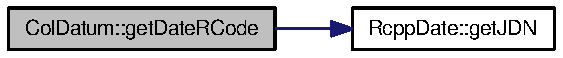
\includegraphics[width=153pt]{classColDatum_87c424137afc43068bf1aba75035851d_cgraph}
\end{center}
\end{figure}
\hypertarget{classColDatum_408e78096b13b5047ae25e99e945ebf6}{
\index{ColDatum@{ColDatum}!getDatetimeValue@{getDatetimeValue}}
\index{getDatetimeValue@{getDatetimeValue}!ColDatum@{ColDatum}}
\subsubsection[{getDatetimeValue}]{\setlength{\rightskip}{0pt plus 5cm}{\bf RcppDatetime} ColDatum::getDatetimeValue ()\hspace{0.3cm}{\tt  \mbox{[}inline\mbox{]}}}}
\label{classColDatum_408e78096b13b5047ae25e99e945ebf6}




Definition at line 260 of file Rcpp.h.

References COLTYPE\_\-DATETIME, type, and x.\hypertarget{classColDatum_70480f53f9cee46bcdaed7331e38c943}{
\index{ColDatum@{ColDatum}!getDateValue@{getDateValue}}
\index{getDateValue@{getDateValue}!ColDatum@{ColDatum}}
\subsubsection[{getDateValue}]{\setlength{\rightskip}{0pt plus 5cm}{\bf RcppDate} ColDatum::getDateValue ()\hspace{0.3cm}{\tt  \mbox{[}inline\mbox{]}}}}
\label{classColDatum_70480f53f9cee46bcdaed7331e38c943}




Definition at line 252 of file Rcpp.h.

References COLTYPE\_\-DATE, d, and type.\hypertarget{classColDatum_6a19044be8ade2b14b372b179210a9bd}{
\index{ColDatum@{ColDatum}!getDoubleValue@{getDoubleValue}}
\index{getDoubleValue@{getDoubleValue}!ColDatum@{ColDatum}}
\subsubsection[{getDoubleValue}]{\setlength{\rightskip}{0pt plus 5cm}double ColDatum::getDoubleValue ()\hspace{0.3cm}{\tt  \mbox{[}inline\mbox{]}}}}
\label{classColDatum_6a19044be8ade2b14b372b179210a9bd}




Definition at line 232 of file Rcpp.h.

References COLTYPE\_\-DOUBLE, type, and x.\hypertarget{classColDatum_df3716db9f3483f3cd255a4c05823479}{
\index{ColDatum@{ColDatum}!getFactorLevel@{getFactorLevel}}
\index{getFactorLevel@{getFactorLevel}!ColDatum@{ColDatum}}
\subsubsection[{getFactorLevel}]{\setlength{\rightskip}{0pt plus 5cm}int ColDatum::getFactorLevel ()\hspace{0.3cm}{\tt  \mbox{[}inline\mbox{]}}}}
\label{classColDatum_df3716db9f3483f3cd255a4c05823479}




Definition at line 271 of file Rcpp.h.

References checkFactorType(), and level.

Here is the call graph for this function:\nopagebreak
\begin{figure}[H]
\begin{center}
\leavevmode
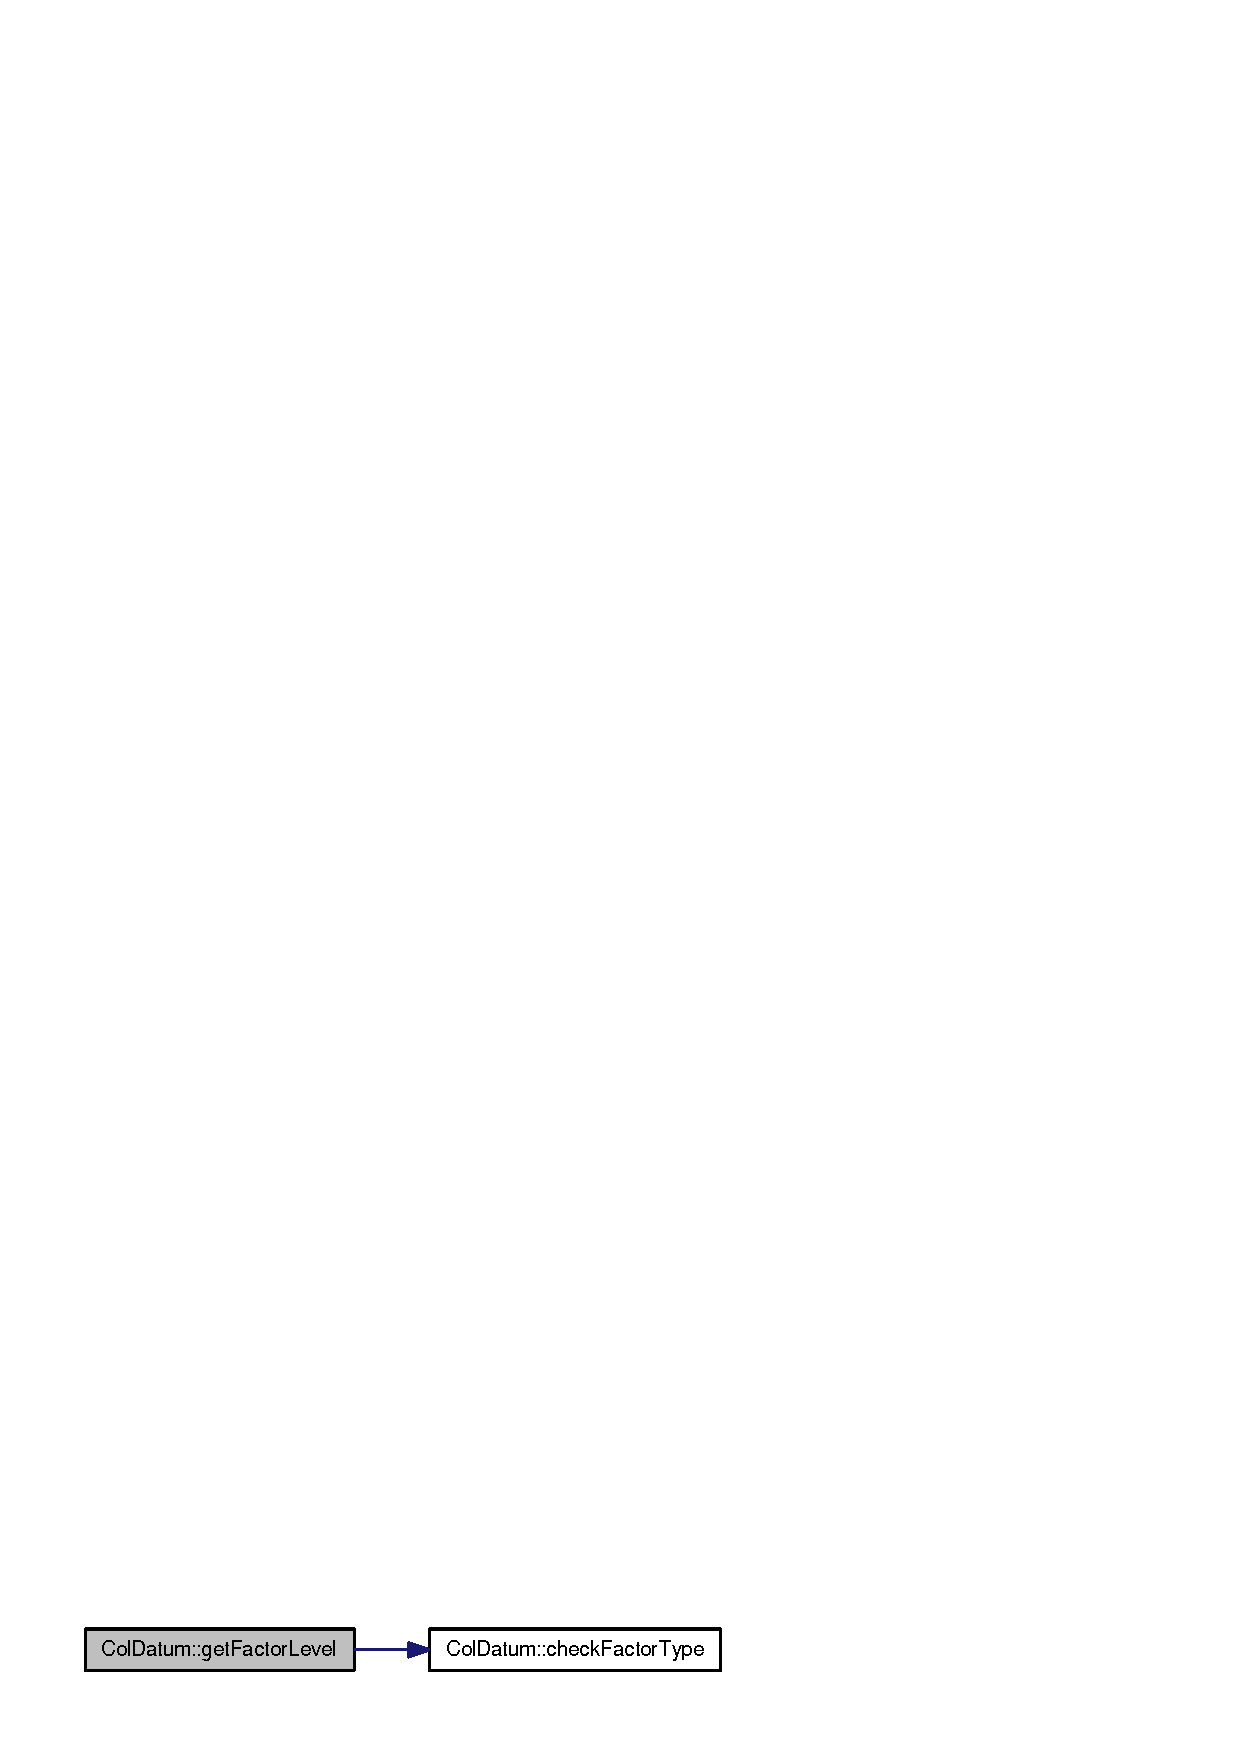
\includegraphics[width=175pt]{classColDatum_df3716db9f3483f3cd255a4c05823479_cgraph}
\end{center}
\end{figure}
\hypertarget{classColDatum_012df5970083052c2348cbda9ed646bb}{
\index{ColDatum@{ColDatum}!getFactorLevelName@{getFactorLevelName}}
\index{getFactorLevelName@{getFactorLevelName}!ColDatum@{ColDatum}}
\subsubsection[{getFactorLevelName}]{\setlength{\rightskip}{0pt plus 5cm}std::string ColDatum::getFactorLevelName ()\hspace{0.3cm}{\tt  \mbox{[}inline\mbox{]}}}}
\label{classColDatum_012df5970083052c2348cbda9ed646bb}




Definition at line 273 of file Rcpp.h.

References checkFactorType(), level, and levelNames.

Here is the call graph for this function:\nopagebreak
\begin{figure}[H]
\begin{center}
\leavevmode
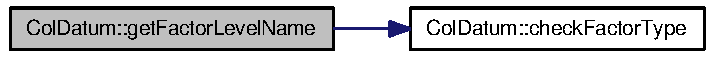
\includegraphics[width=188pt]{classColDatum_012df5970083052c2348cbda9ed646bb_cgraph}
\end{center}
\end{figure}
\hypertarget{classColDatum_4376ad852efcf177fad6f168a8f44877}{
\index{ColDatum@{ColDatum}!getFactorLevelNames@{getFactorLevelNames}}
\index{getFactorLevelNames@{getFactorLevelNames}!ColDatum@{ColDatum}}
\subsubsection[{getFactorLevelNames}]{\setlength{\rightskip}{0pt plus 5cm}std::string$\ast$ ColDatum::getFactorLevelNames ()\hspace{0.3cm}{\tt  \mbox{[}inline\mbox{]}}}}
\label{classColDatum_4376ad852efcf177fad6f168a8f44877}




Definition at line 272 of file Rcpp.h.

References checkFactorType(), and levelNames.

Here is the call graph for this function:\nopagebreak
\begin{figure}[H]
\begin{center}
\leavevmode
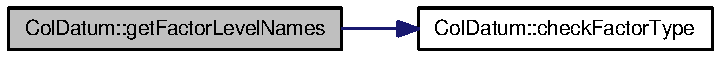
\includegraphics[width=190pt]{classColDatum_4376ad852efcf177fad6f168a8f44877_cgraph}
\end{center}
\end{figure}
\hypertarget{classColDatum_9b5db8254be428e68c61805f02723821}{
\index{ColDatum@{ColDatum}!getFactorNumLevels@{getFactorNumLevels}}
\index{getFactorNumLevels@{getFactorNumLevels}!ColDatum@{ColDatum}}
\subsubsection[{getFactorNumLevels}]{\setlength{\rightskip}{0pt plus 5cm}int ColDatum::getFactorNumLevels ()\hspace{0.3cm}{\tt  \mbox{[}inline\mbox{]}}}}
\label{classColDatum_9b5db8254be428e68c61805f02723821}




Definition at line 270 of file Rcpp.h.

References checkFactorType(), and numLevels.

Here is the call graph for this function:\nopagebreak
\begin{figure}[H]
\begin{center}
\leavevmode
\includegraphics[width=188pt]{classColDatum_9b5db8254be428e68c61805f02723821_cgraph}
\end{center}
\end{figure}
\hypertarget{classColDatum_f498266608526c9db7f865bc66cc5e40}{
\index{ColDatum@{ColDatum}!getIntValue@{getIntValue}}
\index{getIntValue@{getIntValue}!ColDatum@{ColDatum}}
\subsubsection[{getIntValue}]{\setlength{\rightskip}{0pt plus 5cm}int ColDatum::getIntValue ()\hspace{0.3cm}{\tt  \mbox{[}inline\mbox{]}}}}
\label{classColDatum_f498266608526c9db7f865bc66cc5e40}




Definition at line 237 of file Rcpp.h.

References COLTYPE\_\-INT, i, and type.\hypertarget{classColDatum_df81b2aed6f8e19b6f36310288991f38}{
\index{ColDatum@{ColDatum}!getLogicalValue@{getLogicalValue}}
\index{getLogicalValue@{getLogicalValue}!ColDatum@{ColDatum}}
\subsubsection[{getLogicalValue}]{\setlength{\rightskip}{0pt plus 5cm}int ColDatum::getLogicalValue ()\hspace{0.3cm}{\tt  \mbox{[}inline\mbox{]}}}}
\label{classColDatum_df81b2aed6f8e19b6f36310288991f38}




Definition at line 242 of file Rcpp.h.

References COLTYPE\_\-LOGICAL, i, and type.\hypertarget{classColDatum_d0d76d861441151f31cf42acff4b8c0f}{
\index{ColDatum@{ColDatum}!getStringValue@{getStringValue}}
\index{getStringValue@{getStringValue}!ColDatum@{ColDatum}}
\subsubsection[{getStringValue}]{\setlength{\rightskip}{0pt plus 5cm}std::string ColDatum::getStringValue ()\hspace{0.3cm}{\tt  \mbox{[}inline\mbox{]}}}}
\label{classColDatum_d0d76d861441151f31cf42acff4b8c0f}




Definition at line 247 of file Rcpp.h.

References COLTYPE\_\-STRING, s, and type.\hypertarget{classColDatum_ae862d41617b3ae39f88b5b729ccccc3}{
\index{ColDatum@{ColDatum}!getType@{getType}}
\index{getType@{getType}!ColDatum@{ColDatum}}
\subsubsection[{getType}]{\setlength{\rightskip}{0pt plus 5cm}{\bf ColType} ColDatum::getType () const\hspace{0.3cm}{\tt  \mbox{[}inline\mbox{]}}}}
\label{classColDatum_ae862d41617b3ae39f88b5b729ccccc3}




Definition at line 203 of file Rcpp.h.

References type.\hypertarget{classColDatum_5803eb7a89dc467b88d7d412462c6fb5}{
\index{ColDatum@{ColDatum}!setDatetimeValue@{setDatetimeValue}}
\index{setDatetimeValue@{setDatetimeValue}!ColDatum@{ColDatum}}
\subsubsection[{setDatetimeValue}]{\setlength{\rightskip}{0pt plus 5cm}void ColDatum::setDatetimeValue ({\bf RcppDatetime} {\em datetime})\hspace{0.3cm}{\tt  \mbox{[}inline\mbox{]}}}}
\label{classColDatum_5803eb7a89dc467b88d7d412462c6fb5}




Definition at line 217 of file Rcpp.h.

References COLTYPE\_\-DATETIME, RcppDatetime::m\_\-d, type, and x.\hypertarget{classColDatum_988defa165f1d5ab7cde96d2c86c7c69}{
\index{ColDatum@{ColDatum}!setDateValue@{setDateValue}}
\index{setDateValue@{setDateValue}!ColDatum@{ColDatum}}
\subsubsection[{setDateValue}]{\setlength{\rightskip}{0pt plus 5cm}void ColDatum::setDateValue ({\bf RcppDate} {\em date})\hspace{0.3cm}{\tt  \mbox{[}inline\mbox{]}}}}
\label{classColDatum_988defa165f1d5ab7cde96d2c86c7c69}




Definition at line 213 of file Rcpp.h.

References COLTYPE\_\-DATE, d, and type.\hypertarget{classColDatum_edf3ac3ea399222524f02f3468ec97a0}{
\index{ColDatum@{ColDatum}!setDoubleValue@{setDoubleValue}}
\index{setDoubleValue@{setDoubleValue}!ColDatum@{ColDatum}}
\subsubsection[{setDoubleValue}]{\setlength{\rightskip}{0pt plus 5cm}void ColDatum::setDoubleValue (double {\em val})\hspace{0.3cm}{\tt  \mbox{[}inline\mbox{]}}}}
\label{classColDatum_edf3ac3ea399222524f02f3468ec97a0}




Definition at line 205 of file Rcpp.h.

References COLTYPE\_\-DOUBLE, type, and x.\hypertarget{classColDatum_bd6f582044692c2215d9cd4add379ea1}{
\index{ColDatum@{ColDatum}!setFactorValue@{setFactorValue}}
\index{setFactorValue@{setFactorValue}!ColDatum@{ColDatum}}
\subsubsection[{setFactorValue}]{\setlength{\rightskip}{0pt plus 5cm}void ColDatum::setFactorValue (std::string $\ast$ {\em names}, \/  int {\em numNames}, \/  int {\em factorLevel})\hspace{0.3cm}{\tt  \mbox{[}inline\mbox{]}}}}
\label{classColDatum_bd6f582044692c2215d9cd4add379ea1}




Definition at line 221 of file Rcpp.h.

References COLTYPE\_\-FACTOR, i, level, levelNames, numLevels, and type.\hypertarget{classColDatum_80d401e1efb6e714113990c78e72eb84}{
\index{ColDatum@{ColDatum}!setIntValue@{setIntValue}}
\index{setIntValue@{setIntValue}!ColDatum@{ColDatum}}
\subsubsection[{setIntValue}]{\setlength{\rightskip}{0pt plus 5cm}void ColDatum::setIntValue (int {\em val})\hspace{0.3cm}{\tt  \mbox{[}inline\mbox{]}}}}
\label{classColDatum_80d401e1efb6e714113990c78e72eb84}




Definition at line 206 of file Rcpp.h.

References COLTYPE\_\-INT, i, and type.\hypertarget{classColDatum_19ebd9c0e3e2544c8679999ab91c9e20}{
\index{ColDatum@{ColDatum}!setLogicalValue@{setLogicalValue}}
\index{setLogicalValue@{setLogicalValue}!ColDatum@{ColDatum}}
\subsubsection[{setLogicalValue}]{\setlength{\rightskip}{0pt plus 5cm}void ColDatum::setLogicalValue (int {\em val})\hspace{0.3cm}{\tt  \mbox{[}inline\mbox{]}}}}
\label{classColDatum_19ebd9c0e3e2544c8679999ab91c9e20}




Definition at line 207 of file Rcpp.h.

References COLTYPE\_\-LOGICAL, i, and type.\hypertarget{classColDatum_a87060ae6c415167d501c41684d8a586}{
\index{ColDatum@{ColDatum}!setStringValue@{setStringValue}}
\index{setStringValue@{setStringValue}!ColDatum@{ColDatum}}
\subsubsection[{setStringValue}]{\setlength{\rightskip}{0pt plus 5cm}void ColDatum::setStringValue (std::string {\em val})\hspace{0.3cm}{\tt  \mbox{[}inline\mbox{]}}}}
\label{classColDatum_a87060ae6c415167d501c41684d8a586}




Definition at line 212 of file Rcpp.h.

References COLTYPE\_\-STRING, s, and type.

\subsection{Member Data Documentation}
\hypertarget{classColDatum_01a9fd53a56cf0cafa9c3230a3185c8c}{
\index{ColDatum@{ColDatum}!d@{d}}
\index{d@{d}!ColDatum@{ColDatum}}
\subsubsection[{d}]{\setlength{\rightskip}{0pt plus 5cm}{\bf RcppDate} {\bf ColDatum::d}\hspace{0.3cm}{\tt  \mbox{[}private\mbox{]}}}}
\label{classColDatum_01a9fd53a56cf0cafa9c3230a3185c8c}




Definition at line 283 of file Rcpp.h.

Referenced by ColDatum(), getDateRCode(), getDateValue(), and setDateValue().\hypertarget{classColDatum_4ceff4204e29f345957cb5544f40104f}{
\index{ColDatum@{ColDatum}!i@{i}}
\index{i@{i}!ColDatum@{ColDatum}}
\subsubsection[{i}]{\setlength{\rightskip}{0pt plus 5cm}int {\bf ColDatum::i}\hspace{0.3cm}{\tt  \mbox{[}private\mbox{]}}}}
\label{classColDatum_4ceff4204e29f345957cb5544f40104f}




Definition at line 279 of file Rcpp.h.

Referenced by ColDatum(), getIntValue(), getLogicalValue(), setFactorValue(), setIntValue(), and setLogicalValue().\hypertarget{classColDatum_7b0fc92a094e9d1a865fd84c939170d0}{
\index{ColDatum@{ColDatum}!level@{level}}
\index{level@{level}!ColDatum@{ColDatum}}
\subsubsection[{level}]{\setlength{\rightskip}{0pt plus 5cm}int {\bf ColDatum::level}\hspace{0.3cm}{\tt  \mbox{[}private\mbox{]}}}}
\label{classColDatum_7b0fc92a094e9d1a865fd84c939170d0}




Definition at line 280 of file Rcpp.h.

Referenced by ColDatum(), getFactorLevel(), getFactorLevelName(), and setFactorValue().\hypertarget{classColDatum_2abac3c574e1ab36531b03849197f779}{
\index{ColDatum@{ColDatum}!levelNames@{levelNames}}
\index{levelNames@{levelNames}!ColDatum@{ColDatum}}
\subsubsection[{levelNames}]{\setlength{\rightskip}{0pt plus 5cm}std::string$\ast$ {\bf ColDatum::levelNames}\hspace{0.3cm}{\tt  \mbox{[}private\mbox{]}}}}
\label{classColDatum_2abac3c574e1ab36531b03849197f779}




Definition at line 282 of file Rcpp.h.

Referenced by ColDatum(), getFactorLevelName(), getFactorLevelNames(), setFactorValue(), and $\sim$ColDatum().\hypertarget{classColDatum_42954a262993eee014db2d1fd7a7c34f}{
\index{ColDatum@{ColDatum}!numLevels@{numLevels}}
\index{numLevels@{numLevels}!ColDatum@{ColDatum}}
\subsubsection[{numLevels}]{\setlength{\rightskip}{0pt plus 5cm}int {\bf ColDatum::numLevels}\hspace{0.3cm}{\tt  \mbox{[}private\mbox{]}}}}
\label{classColDatum_42954a262993eee014db2d1fd7a7c34f}




Definition at line 281 of file Rcpp.h.

Referenced by ColDatum(), getFactorNumLevels(), and setFactorValue().\hypertarget{classColDatum_5a1c85e1da2da02052078a3c8d810be9}{
\index{ColDatum@{ColDatum}!s@{s}}
\index{s@{s}!ColDatum@{ColDatum}}
\subsubsection[{s}]{\setlength{\rightskip}{0pt plus 5cm}std::string {\bf ColDatum::s}\hspace{0.3cm}{\tt  \mbox{[}private\mbox{]}}}}
\label{classColDatum_5a1c85e1da2da02052078a3c8d810be9}




Definition at line 277 of file Rcpp.h.

Referenced by ColDatum(), getStringValue(), and setStringValue().\hypertarget{classColDatum_c539e7f62828f2683f1825a84a19d231}{
\index{ColDatum@{ColDatum}!type@{type}}
\index{type@{type}!ColDatum@{ColDatum}}
\subsubsection[{type}]{\setlength{\rightskip}{0pt plus 5cm}{\bf ColType} {\bf ColDatum::type}\hspace{0.3cm}{\tt  \mbox{[}private\mbox{]}}}}
\label{classColDatum_c539e7f62828f2683f1825a84a19d231}




Definition at line 276 of file Rcpp.h.

Referenced by checkFactorType(), ColDatum(), getDatetimeValue(), getDateValue(), getDoubleValue(), getIntValue(), getLogicalValue(), getStringValue(), getType(), setDatetimeValue(), setDateValue(), setDoubleValue(), setFactorValue(), setIntValue(), setLogicalValue(), setStringValue(), and $\sim$ColDatum().\hypertarget{classColDatum_6d3d286cbd6c4ad24f1f12266662e42e}{
\index{ColDatum@{ColDatum}!x@{x}}
\index{x@{x}!ColDatum@{ColDatum}}
\subsubsection[{x}]{\setlength{\rightskip}{0pt plus 5cm}double {\bf ColDatum::x}\hspace{0.3cm}{\tt  \mbox{[}private\mbox{]}}}}
\label{classColDatum_6d3d286cbd6c4ad24f1f12266662e42e}




Definition at line 278 of file Rcpp.h.

Referenced by ColDatum(), getDatetimeValue(), getDoubleValue(), setDatetimeValue(), and setDoubleValue().

The documentation for this class was generated from the following file:\begin{CompactItemize}
\item 
src/\hyperlink{Rcpp_8h}{Rcpp.h}\end{CompactItemize}

\hypertarget{classMyRListFunc}{
\section{MyRListFunc Class Reference}
\label{classMyRListFunc}\index{MyRListFunc@{MyRListFunc}}
}
Inherits \hyperlink{classRcppFunction}{RcppFunction}.

Collaboration diagram for MyRListFunc:\nopagebreak
\begin{figure}[H]
\begin{center}
\leavevmode
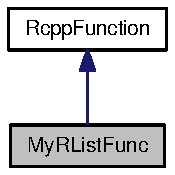
\includegraphics[width=120pt]{classMyRListFunc__coll__graph}
\end{center}
\end{figure}
\subsection*{Public Member Functions}
\begin{CompactItemize}
\item 
\hyperlink{classMyRListFunc_7ab78b186d110497a404f88009455af6}{MyRListFunc} (SEXP \hyperlink{classRcppFunction_a6b5966224b8b7d158be6cdfc3612063}{fn})
\item 
std::vector$<$ double $>$ \hyperlink{classMyRListFunc_0dec3b59e1e235c0502594a5d92cae13}{addOne} (double alpha, double beta, double gamma)
\end{CompactItemize}


\subsection{Detailed Description}


Definition at line 78 of file RcppExample.cpp.

\subsection{Constructor \& Destructor Documentation}
\hypertarget{classMyRListFunc_7ab78b186d110497a404f88009455af6}{
\index{MyRListFunc@{MyRListFunc}!MyRListFunc@{MyRListFunc}}
\index{MyRListFunc@{MyRListFunc}!MyRListFunc@{MyRListFunc}}
\subsubsection[{MyRListFunc}]{\setlength{\rightskip}{0pt plus 5cm}MyRListFunc::MyRListFunc (SEXP {\em fn})\hspace{0.3cm}{\tt  \mbox{[}inline\mbox{]}}}}
\label{classMyRListFunc_7ab78b186d110497a404f88009455af6}




Definition at line 80 of file RcppExample.cpp.

\subsection{Member Function Documentation}
\hypertarget{classMyRListFunc_0dec3b59e1e235c0502594a5d92cae13}{
\index{MyRListFunc@{MyRListFunc}!addOne@{addOne}}
\index{addOne@{addOne}!MyRListFunc@{MyRListFunc}}
\subsubsection[{addOne}]{\setlength{\rightskip}{0pt plus 5cm}std::vector$<$double$>$ MyRListFunc::addOne (double {\em alpha}, \/  double {\em beta}, \/  double {\em gamma})\hspace{0.3cm}{\tt  \mbox{[}inline\mbox{]}}}}
\label{classMyRListFunc_0dec3b59e1e235c0502594a5d92cae13}




Definition at line 81 of file RcppExample.cpp.

References RcppFunction::appendToRList(), RcppFunction::clearProtectionStack(), RcppFunction::listCall(), and RcppFunction::setRListSize().

Referenced by Rcpp\_\-Example().

Here is the call graph for this function:\nopagebreak
\begin{figure}[H]
\begin{center}
\leavevmode
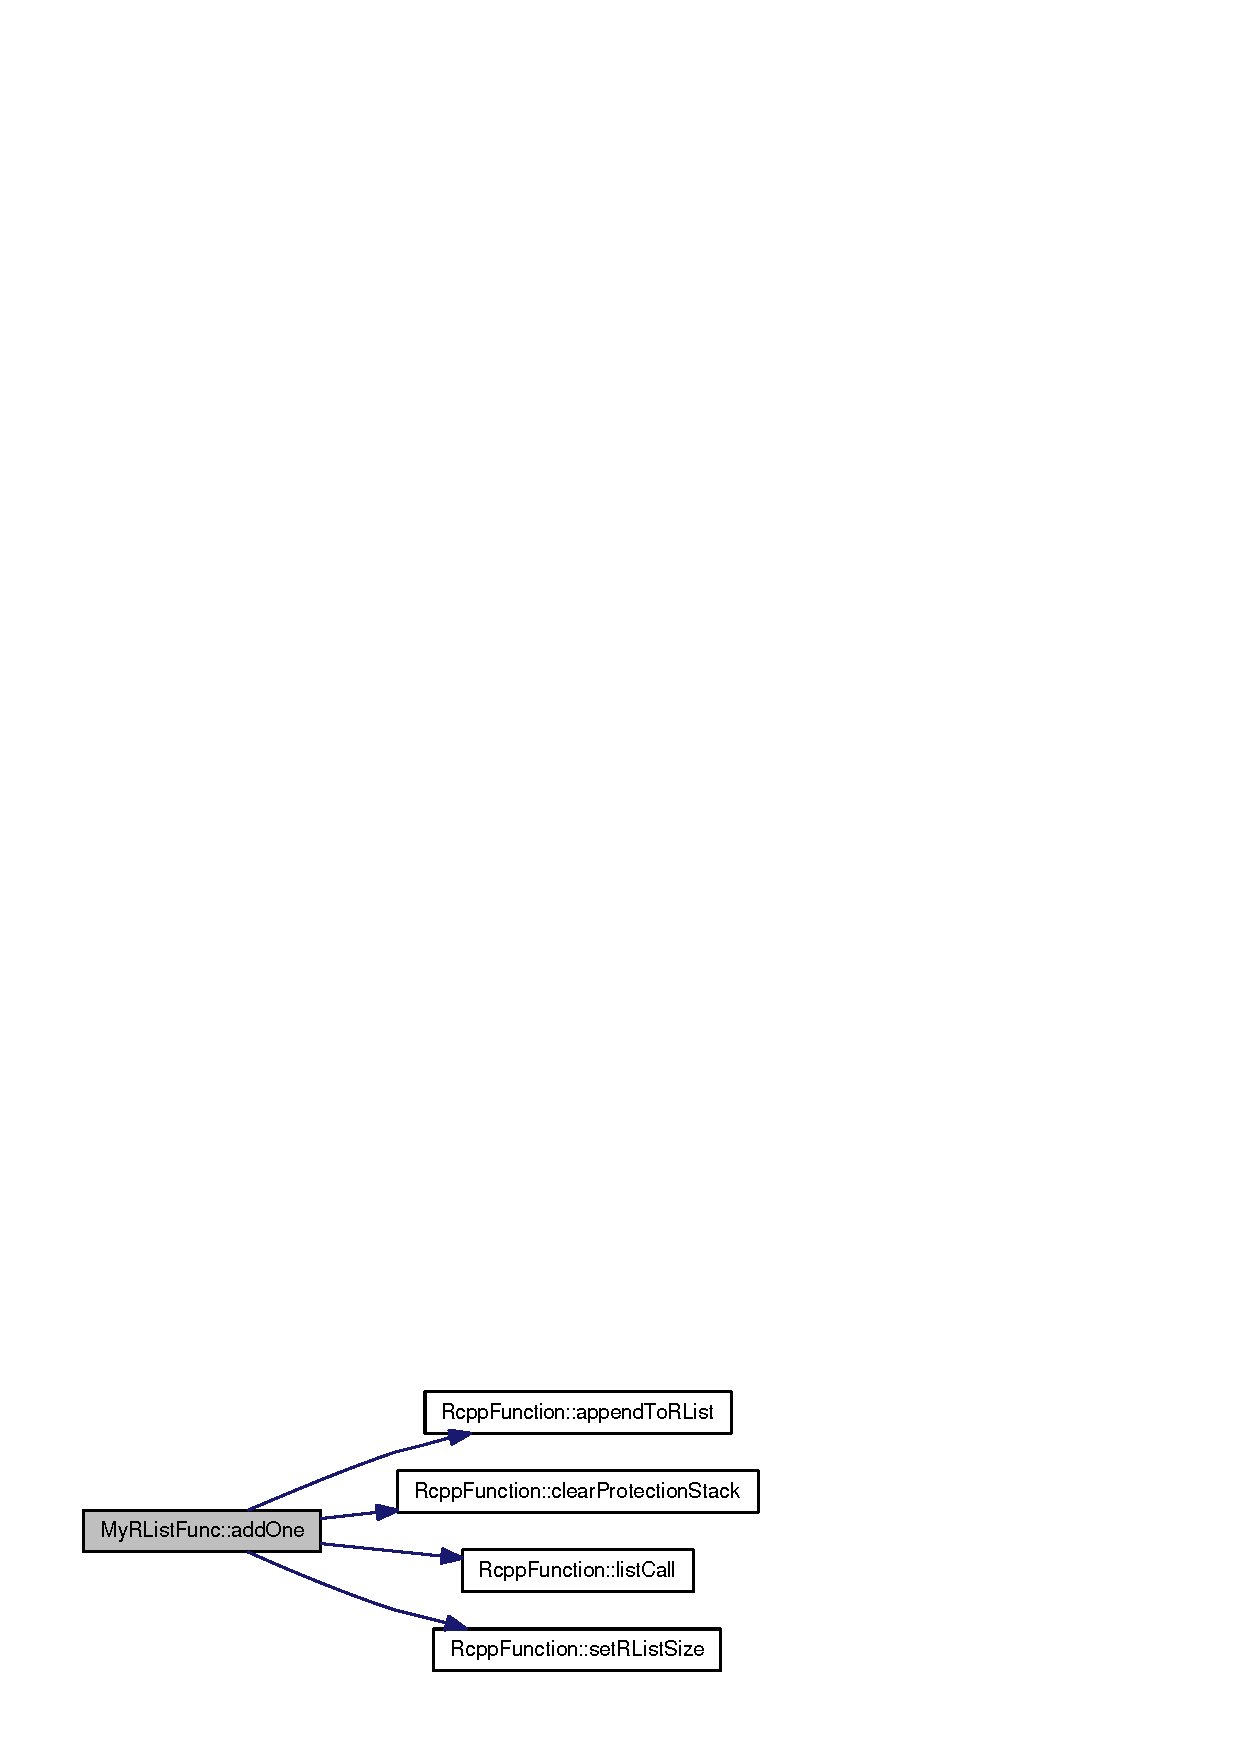
\includegraphics[width=184pt]{classMyRListFunc_0dec3b59e1e235c0502594a5d92cae13_cgraph}
\end{center}
\end{figure}


The documentation for this class was generated from the following file:\begin{CompactItemize}
\item 
src/\hyperlink{RcppExample_8cpp}{RcppExample.cpp}\end{CompactItemize}

\hypertarget{classMyRVectorFunc}{
\section{MyRVectorFunc Class Reference}
\label{classMyRVectorFunc}\index{MyRVectorFunc@{MyRVectorFunc}}
}
Inheritance diagram for MyRVectorFunc:\nopagebreak
\begin{figure}[H]
\begin{center}
\leavevmode
\includegraphics[width=65pt]{classMyRVectorFunc__inherit__graph}
\end{center}
\end{figure}
Collaboration diagram for MyRVectorFunc:\nopagebreak
\begin{figure}[H]
\begin{center}
\leavevmode
\includegraphics[width=65pt]{classMyRVectorFunc__coll__graph}
\end{center}
\end{figure}
\subsection*{Public Member Functions}
\begin{CompactItemize}
\item 
\hyperlink{classMyRVectorFunc_dc09bab76bddb0c246ed98c942fd4cd8}{MyRVectorFunc} (SEXP \hyperlink{classRcppFunction_a6b5966224b8b7d158be6cdfc3612063}{fn})
\item 
double \hyperlink{classMyRVectorFunc_2eba5a390ca620a687e77208bfbb6df4}{getSum} (std::vector$<$ double $>$ \&v)
\end{CompactItemize}


\subsection{Detailed Description}


Definition at line 36 of file RcppExample.cpp.

\subsection{Constructor \& Destructor Documentation}
\hypertarget{classMyRVectorFunc_dc09bab76bddb0c246ed98c942fd4cd8}{
\index{MyRVectorFunc@{MyRVectorFunc}!MyRVectorFunc@{MyRVectorFunc}}
\index{MyRVectorFunc@{MyRVectorFunc}!MyRVectorFunc@{MyRVectorFunc}}
\subsubsection[MyRVectorFunc]{\setlength{\rightskip}{0pt plus 5cm}MyRVectorFunc::MyRVectorFunc (SEXP {\em fn})\hspace{0.3cm}{\tt  \mbox{[}inline\mbox{]}}}}
\label{classMyRVectorFunc_dc09bab76bddb0c246ed98c942fd4cd8}




Definition at line 38 of file RcppExample.cpp.

\subsection{Member Function Documentation}
\hypertarget{classMyRVectorFunc_2eba5a390ca620a687e77208bfbb6df4}{
\index{MyRVectorFunc@{MyRVectorFunc}!getSum@{getSum}}
\index{getSum@{getSum}!MyRVectorFunc@{MyRVectorFunc}}
\subsubsection[getSum]{\setlength{\rightskip}{0pt plus 5cm}double MyRVectorFunc::getSum (std::vector$<$ double $>$ \& {\em v})\hspace{0.3cm}{\tt  \mbox{[}inline\mbox{]}}}}
\label{classMyRVectorFunc_2eba5a390ca620a687e77208bfbb6df4}




Definition at line 42 of file RcppExample.cpp.

References RcppFunction::clearProtectionStack(), RcppFunction::setRVector(), and RcppFunction::vectorCall().

Referenced by Rcpp\_\-Example().

Here is the call graph for this function:\nopagebreak
\begin{figure}[H]
\begin{center}
\leavevmode
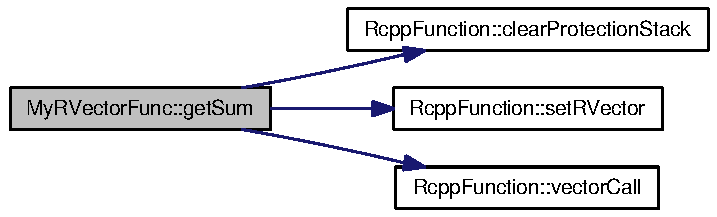
\includegraphics[width=190pt]{classMyRVectorFunc_2eba5a390ca620a687e77208bfbb6df4_cgraph}
\end{center}
\end{figure}


The documentation for this class was generated from the following file:\begin{CompactItemize}
\item 
src/\hyperlink{RcppExample_8cpp}{RcppExample.cpp}\end{CompactItemize}

\hypertarget{classRcppDate}{
\section{RcppDate Class Reference}
\label{classRcppDate}\index{RcppDate@{RcppDate}}
}
{\tt \#include $<$Rcpp.h$>$}

\subsection*{Public Member Functions}
\begin{CompactItemize}
\item 
\hyperlink{classRcppDate_4f0f6ae9e9e284fd058d615bcd78d6f9}{RcppDate} ()
\item 
\hyperlink{classRcppDate_21adf306ddf84cf792f888d220bb9a3f}{RcppDate} (int Rjdn)
\item 
\hyperlink{classRcppDate_8b96145664d63ec84267870787025fa4}{RcppDate} (int month\_\-, int day\_\-, int year\_\-)
\item 
int \hyperlink{classRcppDate_16ca2d57a2c4047b027c8b8b0db5184f}{getMonth} () const 
\item 
int \hyperlink{classRcppDate_20efbcdddceac536425407b3169fff5a}{getDay} () const 
\item 
int \hyperlink{classRcppDate_79a7696fbce7b448ab545ce35c40811b}{getYear} () const 
\item 
int \hyperlink{classRcppDate_71332de00640903fe99ce13a37fd9f67}{getJDN} () const 
\end{CompactItemize}
\subsection*{Static Public Attributes}
\begin{CompactItemize}
\item 
static const int \hyperlink{classRcppDate_44b0643ab19489a0fb9700d25f504902}{Jan1970Offset} = 2440588
\item 
static const int \hyperlink{classRcppDate_06b285d4a04c5225a067e76d4fbfd2d4}{QLtoJan1970Offset} = 25569
\end{CompactItemize}
\subsection*{Private Member Functions}
\begin{CompactItemize}
\item 
void \hyperlink{classRcppDate_aaa626a51e3b2eb4978caf5dcdf9df70}{mdy2jdn} ()
\item 
void \hyperlink{classRcppDate_ca9e6ccbf5bf76e9bba92f2a3083c135}{jdn2mdy} ()
\end{CompactItemize}
\subsection*{Private Attributes}
\begin{CompactItemize}
\item 
int \hyperlink{classRcppDate_00bf3ece7320d63aee4f6b6df82b4f63}{month}
\item 
int \hyperlink{classRcppDate_9e6aec176d9432829a304550eadd4205}{day}
\item 
int \hyperlink{classRcppDate_8881f654ebf42cdf71fdcfce402f0cad}{year}
\item 
int \hyperlink{classRcppDate_b883f696379dd06e39c6c9b3502a2164}{jdn}
\end{CompactItemize}
\subsection*{Friends}
\begin{CompactItemize}
\item 
\hyperlink{classRcppDate}{RcppDate} \hyperlink{classRcppDate_dd881a27c2b8e36897a59bca1d04585f}{operator+} (const \hyperlink{classRcppDate}{RcppDate} \&date, int offset)
\item 
int \hyperlink{classRcppDate_49241820910c75948937f70f76c0849d}{operator-} (const \hyperlink{classRcppDate}{RcppDate} \&date1, const \hyperlink{classRcppDate}{RcppDate} \&date2)
\item 
bool \hyperlink{classRcppDate_f852d3a1ad52776201f385be5ea18c71}{operator$<$} (const \hyperlink{classRcppDate}{RcppDate} \&date1, const \hyperlink{classRcppDate}{RcppDate} \&date2)
\item 
bool \hyperlink{classRcppDate_80164a177c098301c1d509fdab702567}{operator$>$} (const \hyperlink{classRcppDate}{RcppDate} \&date1, const \hyperlink{classRcppDate}{RcppDate} \&date2)
\item 
bool \hyperlink{classRcppDate_d6c1518c6eb9480665f532dbcc6dd2d5}{operator==} (const \hyperlink{classRcppDate}{RcppDate} \&date1, const \hyperlink{classRcppDate}{RcppDate} \&date2)
\item 
bool \hyperlink{classRcppDate_f7a217e1f5d4a91e2d86fc4da858a6c2}{operator$>$=} (const \hyperlink{classRcppDate}{RcppDate} \&date1, const \hyperlink{classRcppDate}{RcppDate} \&date2)
\item 
bool \hyperlink{classRcppDate_594132f5ef49b4f477d32289ced4df83}{operator$<$=} (const \hyperlink{classRcppDate}{RcppDate} \&date1, const \hyperlink{classRcppDate}{RcppDate} \&date2)
\item 
std::ostream \& \hyperlink{classRcppDate_62c075d47528a48e5fb57c1855c4d71c}{operator$<$$<$} (std::ostream \&os, const \hyperlink{classRcppDate}{RcppDate} \&date)
\end{CompactItemize}


\subsection{Detailed Description}


Definition at line 47 of file Rcpp.h.

\subsection{Constructor \& Destructor Documentation}
\hypertarget{classRcppDate_4f0f6ae9e9e284fd058d615bcd78d6f9}{
\index{RcppDate@{RcppDate}!RcppDate@{RcppDate}}
\index{RcppDate@{RcppDate}!RcppDate@{RcppDate}}
\subsubsection[{RcppDate}]{\setlength{\rightskip}{0pt plus 5cm}RcppDate::RcppDate ()\hspace{0.3cm}{\tt  \mbox{[}inline\mbox{]}}}}
\label{classRcppDate_4f0f6ae9e9e284fd058d615bcd78d6f9}




Definition at line 57 of file Rcpp.h.

References day, mdy2jdn(), month, and year.

Here is the call graph for this function:\nopagebreak
\begin{figure}[H]
\begin{center}
\leavevmode
\includegraphics[width=145pt]{classRcppDate_4f0f6ae9e9e284fd058d615bcd78d6f9_cgraph}
\end{center}
\end{figure}
\hypertarget{classRcppDate_21adf306ddf84cf792f888d220bb9a3f}{
\index{RcppDate@{RcppDate}!RcppDate@{RcppDate}}
\index{RcppDate@{RcppDate}!RcppDate@{RcppDate}}
\subsubsection[{RcppDate}]{\setlength{\rightskip}{0pt plus 5cm}RcppDate::RcppDate (int {\em Rjdn})\hspace{0.3cm}{\tt  \mbox{[}inline\mbox{]}}}}
\label{classRcppDate_21adf306ddf84cf792f888d220bb9a3f}




Definition at line 58 of file Rcpp.h.

References Jan1970Offset, jdn, and jdn2mdy().

Here is the call graph for this function:\nopagebreak
\begin{figure}[H]
\begin{center}
\leavevmode
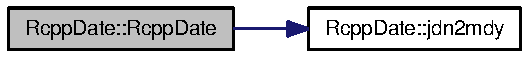
\includegraphics[width=145pt]{classRcppDate_21adf306ddf84cf792f888d220bb9a3f_cgraph}
\end{center}
\end{figure}
\hypertarget{classRcppDate_8b96145664d63ec84267870787025fa4}{
\index{RcppDate@{RcppDate}!RcppDate@{RcppDate}}
\index{RcppDate@{RcppDate}!RcppDate@{RcppDate}}
\subsubsection[{RcppDate}]{\setlength{\rightskip}{0pt plus 5cm}RcppDate::RcppDate (int {\em month\_\-}, \/  int {\em day\_\-}, \/  int {\em year\_\-})\hspace{0.3cm}{\tt  \mbox{[}inline\mbox{]}}}}
\label{classRcppDate_8b96145664d63ec84267870787025fa4}




Definition at line 59 of file Rcpp.h.

References mdy2jdn().

Here is the call graph for this function:\nopagebreak
\begin{figure}[H]
\begin{center}
\leavevmode
\includegraphics[width=145pt]{classRcppDate_8b96145664d63ec84267870787025fa4_cgraph}
\end{center}
\end{figure}


\subsection{Member Function Documentation}
\hypertarget{classRcppDate_20efbcdddceac536425407b3169fff5a}{
\index{RcppDate@{RcppDate}!getDay@{getDay}}
\index{getDay@{getDay}!RcppDate@{RcppDate}}
\subsubsection[{getDay}]{\setlength{\rightskip}{0pt plus 5cm}int RcppDate::getDay () const\hspace{0.3cm}{\tt  \mbox{[}inline\mbox{]}}}}
\label{classRcppDate_20efbcdddceac536425407b3169fff5a}




Definition at line 67 of file Rcpp.h.

References day.

Referenced by operator$<$$<$(), Rcpp\_\-Example(), and RcppParamsExample().\hypertarget{classRcppDate_71332de00640903fe99ce13a37fd9f67}{
\index{RcppDate@{RcppDate}!getJDN@{getJDN}}
\index{getJDN@{getJDN}!RcppDate@{RcppDate}}
\subsubsection[{getJDN}]{\setlength{\rightskip}{0pt plus 5cm}int RcppDate::getJDN () const\hspace{0.3cm}{\tt  \mbox{[}inline\mbox{]}}}}
\label{classRcppDate_71332de00640903fe99ce13a37fd9f67}




Definition at line 69 of file Rcpp.h.

References jdn.

Referenced by RcppResultSet::add(), RcppFunction::appendToRList(), and ColDatum::getDateRCode().\hypertarget{classRcppDate_16ca2d57a2c4047b027c8b8b0db5184f}{
\index{RcppDate@{RcppDate}!getMonth@{getMonth}}
\index{getMonth@{getMonth}!RcppDate@{RcppDate}}
\subsubsection[{getMonth}]{\setlength{\rightskip}{0pt plus 5cm}int RcppDate::getMonth () const\hspace{0.3cm}{\tt  \mbox{[}inline\mbox{]}}}}
\label{classRcppDate_16ca2d57a2c4047b027c8b8b0db5184f}




Definition at line 66 of file Rcpp.h.

References month.

Referenced by operator$<$$<$(), Rcpp\_\-Example(), and RcppParamsExample().\hypertarget{classRcppDate_79a7696fbce7b448ab545ce35c40811b}{
\index{RcppDate@{RcppDate}!getYear@{getYear}}
\index{getYear@{getYear}!RcppDate@{RcppDate}}
\subsubsection[{getYear}]{\setlength{\rightskip}{0pt plus 5cm}int RcppDate::getYear () const\hspace{0.3cm}{\tt  \mbox{[}inline\mbox{]}}}}
\label{classRcppDate_79a7696fbce7b448ab545ce35c40811b}




Definition at line 68 of file Rcpp.h.

References year.

Referenced by operator$<$$<$(), Rcpp\_\-Example(), and RcppParamsExample().\hypertarget{classRcppDate_ca9e6ccbf5bf76e9bba92f2a3083c135}{
\index{RcppDate@{RcppDate}!jdn2mdy@{jdn2mdy}}
\index{jdn2mdy@{jdn2mdy}!RcppDate@{RcppDate}}
\subsubsection[{jdn2mdy}]{\setlength{\rightskip}{0pt plus 5cm}void RcppDate::jdn2mdy ()\hspace{0.3cm}{\tt  \mbox{[}private\mbox{]}}}}
\label{classRcppDate_ca9e6ccbf5bf76e9bba92f2a3083c135}




Definition at line 865 of file Rcpp.cpp.

References day, jdn, month, and year.

Referenced by operator+(), and RcppDate().\hypertarget{classRcppDate_aaa626a51e3b2eb4978caf5dcdf9df70}{
\index{RcppDate@{RcppDate}!mdy2jdn@{mdy2jdn}}
\index{mdy2jdn@{mdy2jdn}!RcppDate@{RcppDate}}
\subsubsection[{mdy2jdn}]{\setlength{\rightskip}{0pt plus 5cm}void RcppDate::mdy2jdn ()\hspace{0.3cm}{\tt  \mbox{[}private\mbox{]}}}}
\label{classRcppDate_aaa626a51e3b2eb4978caf5dcdf9df70}




Definition at line 855 of file Rcpp.cpp.

References day, jdn, month, and year.

Referenced by RcppDate().

\subsection{Friends And Related Function Documentation}
\hypertarget{classRcppDate_dd881a27c2b8e36897a59bca1d04585f}{
\index{RcppDate@{RcppDate}!operator+@{operator+}}
\index{operator+@{operator+}!RcppDate@{RcppDate}}
\subsubsection[{operator+}]{\setlength{\rightskip}{0pt plus 5cm}{\bf RcppDate} operator+ (const {\bf RcppDate} \& {\em date}, \/  int {\em offset})\hspace{0.3cm}{\tt  \mbox{[}friend\mbox{]}}}}
\label{classRcppDate_dd881a27c2b8e36897a59bca1d04585f}




Definition at line 805 of file Rcpp.cpp.\hypertarget{classRcppDate_49241820910c75948937f70f76c0849d}{
\index{RcppDate@{RcppDate}!operator-@{operator-}}
\index{operator-@{operator-}!RcppDate@{RcppDate}}
\subsubsection[{operator-}]{\setlength{\rightskip}{0pt plus 5cm}int operator- (const {\bf RcppDate} \& {\em date1}, \/  const {\bf RcppDate} \& {\em date2})\hspace{0.3cm}{\tt  \mbox{[}friend\mbox{]}}}}
\label{classRcppDate_49241820910c75948937f70f76c0849d}




Definition at line 812 of file Rcpp.cpp.\hypertarget{classRcppDate_f852d3a1ad52776201f385be5ea18c71}{
\index{RcppDate@{RcppDate}!operator$<$@{operator$<$}}
\index{operator$<$@{operator$<$}!RcppDate@{RcppDate}}
\subsubsection[{operator$<$}]{\setlength{\rightskip}{0pt plus 5cm}bool operator$<$ (const {\bf RcppDate} \& {\em date1}, \/  const {\bf RcppDate} \& {\em date2})\hspace{0.3cm}{\tt  \mbox{[}friend\mbox{]}}}}
\label{classRcppDate_f852d3a1ad52776201f385be5ea18c71}




Definition at line 816 of file Rcpp.cpp.\hypertarget{classRcppDate_62c075d47528a48e5fb57c1855c4d71c}{
\index{RcppDate@{RcppDate}!operator$<$$<$@{operator$<$$<$}}
\index{operator$<$$<$@{operator$<$$<$}!RcppDate@{RcppDate}}
\subsubsection[{operator$<$$<$}]{\setlength{\rightskip}{0pt plus 5cm}std::ostream\& operator$<$$<$ (std::ostream \& {\em os}, \/  const {\bf RcppDate} \& {\em date})\hspace{0.3cm}{\tt  \mbox{[}friend\mbox{]}}}}
\label{classRcppDate_62c075d47528a48e5fb57c1855c4d71c}




Definition at line 799 of file Rcpp.cpp.\hypertarget{classRcppDate_594132f5ef49b4f477d32289ced4df83}{
\index{RcppDate@{RcppDate}!operator$<$=@{operator$<$=}}
\index{operator$<$=@{operator$<$=}!RcppDate@{RcppDate}}
\subsubsection[{operator$<$=}]{\setlength{\rightskip}{0pt plus 5cm}bool operator$<$= (const {\bf RcppDate} \& {\em date1}, \/  const {\bf RcppDate} \& {\em date2})\hspace{0.3cm}{\tt  \mbox{[}friend\mbox{]}}}}
\label{classRcppDate_594132f5ef49b4f477d32289ced4df83}




Definition at line 828 of file Rcpp.cpp.\hypertarget{classRcppDate_d6c1518c6eb9480665f532dbcc6dd2d5}{
\index{RcppDate@{RcppDate}!operator==@{operator==}}
\index{operator==@{operator==}!RcppDate@{RcppDate}}
\subsubsection[{operator==}]{\setlength{\rightskip}{0pt plus 5cm}bool operator== (const {\bf RcppDate} \& {\em date1}, \/  const {\bf RcppDate} \& {\em date2})\hspace{0.3cm}{\tt  \mbox{[}friend\mbox{]}}}}
\label{classRcppDate_d6c1518c6eb9480665f532dbcc6dd2d5}




Definition at line 832 of file Rcpp.cpp.\hypertarget{classRcppDate_80164a177c098301c1d509fdab702567}{
\index{RcppDate@{RcppDate}!operator$>$@{operator$>$}}
\index{operator$>$@{operator$>$}!RcppDate@{RcppDate}}
\subsubsection[{operator$>$}]{\setlength{\rightskip}{0pt plus 5cm}bool operator$>$ (const {\bf RcppDate} \& {\em date1}, \/  const {\bf RcppDate} \& {\em date2})\hspace{0.3cm}{\tt  \mbox{[}friend\mbox{]}}}}
\label{classRcppDate_80164a177c098301c1d509fdab702567}




Definition at line 820 of file Rcpp.cpp.\hypertarget{classRcppDate_f7a217e1f5d4a91e2d86fc4da858a6c2}{
\index{RcppDate@{RcppDate}!operator$>$=@{operator$>$=}}
\index{operator$>$=@{operator$>$=}!RcppDate@{RcppDate}}
\subsubsection[{operator$>$=}]{\setlength{\rightskip}{0pt plus 5cm}bool operator$>$= (const {\bf RcppDate} \& {\em date1}, \/  const {\bf RcppDate} \& {\em date2})\hspace{0.3cm}{\tt  \mbox{[}friend\mbox{]}}}}
\label{classRcppDate_f7a217e1f5d4a91e2d86fc4da858a6c2}




Definition at line 824 of file Rcpp.cpp.

\subsection{Member Data Documentation}
\hypertarget{classRcppDate_9e6aec176d9432829a304550eadd4205}{
\index{RcppDate@{RcppDate}!day@{day}}
\index{day@{day}!RcppDate@{RcppDate}}
\subsubsection[{day}]{\setlength{\rightskip}{0pt plus 5cm}int {\bf RcppDate::day}\hspace{0.3cm}{\tt  \mbox{[}private\mbox{]}}}}
\label{classRcppDate_9e6aec176d9432829a304550eadd4205}




Definition at line 51 of file Rcpp.h.

Referenced by getDay(), jdn2mdy(), mdy2jdn(), operator+(), and RcppDate().\hypertarget{classRcppDate_44b0643ab19489a0fb9700d25f504902}{
\index{RcppDate@{RcppDate}!Jan1970Offset@{Jan1970Offset}}
\index{Jan1970Offset@{Jan1970Offset}!RcppDate@{RcppDate}}
\subsubsection[{Jan1970Offset}]{\setlength{\rightskip}{0pt plus 5cm}const int {\bf RcppDate::Jan1970Offset} = 2440588\hspace{0.3cm}{\tt  \mbox{[}static\mbox{]}}}}
\label{classRcppDate_44b0643ab19489a0fb9700d25f504902}




Definition at line 55 of file Rcpp.h.

Referenced by RcppResultSet::add(), RcppFunction::appendToRList(), ColDatum::getDateRCode(), and RcppDate().\hypertarget{classRcppDate_b883f696379dd06e39c6c9b3502a2164}{
\index{RcppDate@{RcppDate}!jdn@{jdn}}
\index{jdn@{jdn}!RcppDate@{RcppDate}}
\subsubsection[{jdn}]{\setlength{\rightskip}{0pt plus 5cm}int {\bf RcppDate::jdn}\hspace{0.3cm}{\tt  \mbox{[}private\mbox{]}}}}
\label{classRcppDate_b883f696379dd06e39c6c9b3502a2164}




Definition at line 52 of file Rcpp.h.

Referenced by getJDN(), jdn2mdy(), mdy2jdn(), operator+(), operator-(), operator$<$(), operator$<$=(), operator==(), operator$>$(), operator$>$=(), and RcppDate().\hypertarget{classRcppDate_00bf3ece7320d63aee4f6b6df82b4f63}{
\index{RcppDate@{RcppDate}!month@{month}}
\index{month@{month}!RcppDate@{RcppDate}}
\subsubsection[{month}]{\setlength{\rightskip}{0pt plus 5cm}int {\bf RcppDate::month}\hspace{0.3cm}{\tt  \mbox{[}private\mbox{]}}}}
\label{classRcppDate_00bf3ece7320d63aee4f6b6df82b4f63}




Definition at line 51 of file Rcpp.h.

Referenced by getMonth(), jdn2mdy(), mdy2jdn(), operator+(), and RcppDate().\hypertarget{classRcppDate_06b285d4a04c5225a067e76d4fbfd2d4}{
\index{RcppDate@{RcppDate}!QLtoJan1970Offset@{QLtoJan1970Offset}}
\index{QLtoJan1970Offset@{QLtoJan1970Offset}!RcppDate@{RcppDate}}
\subsubsection[{QLtoJan1970Offset}]{\setlength{\rightskip}{0pt plus 5cm}const int {\bf RcppDate::QLtoJan1970Offset} = 25569\hspace{0.3cm}{\tt  \mbox{[}static\mbox{]}}}}
\label{classRcppDate_06b285d4a04c5225a067e76d4fbfd2d4}




Definition at line 56 of file Rcpp.h.\hypertarget{classRcppDate_8881f654ebf42cdf71fdcfce402f0cad}{
\index{RcppDate@{RcppDate}!year@{year}}
\index{year@{year}!RcppDate@{RcppDate}}
\subsubsection[{year}]{\setlength{\rightskip}{0pt plus 5cm}int {\bf RcppDate::year}\hspace{0.3cm}{\tt  \mbox{[}private\mbox{]}}}}
\label{classRcppDate_8881f654ebf42cdf71fdcfce402f0cad}




Definition at line 51 of file Rcpp.h.

Referenced by getYear(), jdn2mdy(), mdy2jdn(), operator+(), and RcppDate().

The documentation for this class was generated from the following files:\begin{CompactItemize}
\item 
src/\hyperlink{Rcpp_8h}{Rcpp.h}\item 
src/\hyperlink{Rcpp_8cpp}{Rcpp.cpp}\end{CompactItemize}

\hypertarget{classRcppDatetime}{
\section{RcppDatetime Class Reference}
\label{classRcppDatetime}\index{RcppDatetime@{RcppDatetime}}
}
{\tt \#include $<$Rcpp.h$>$}

\subsection*{Public Member Functions}
\begin{CompactItemize}
\item 
\hyperlink{classRcppDatetime_5a1679444e775781bf038553ef3b04ae}{RcppDatetime} (void)
\item 
\hyperlink{classRcppDatetime_43972d46cd15e6cb666d61f13bdc31f2}{RcppDatetime} (const double d)
\item 
double \hyperlink{classRcppDatetime_cb74d27387c0d851414e20d30354ac62}{getFractionalTimestamp} (void) const 
\item 
int \hyperlink{classRcppDatetime_ba930a8d7d575eb10444258a442027cf}{getYear} (void)
\item 
int \hyperlink{classRcppDatetime_a7f04947d2a27e4bba2d19efa21771ed}{getMonth} (void)
\item 
int \hyperlink{classRcppDatetime_23e9f09bef162e1ffef0e43f8a446b77}{getDay} (void)
\item 
int \hyperlink{classRcppDatetime_796802561fa8bb87a8e2a1836afaaa58}{getWeekday} (void)
\item 
int \hyperlink{classRcppDatetime_0da8db1ecd235a6e7ab309e70e4e93b0}{getHour} (void)
\item 
int \hyperlink{classRcppDatetime_db41bd524ead66d69e129b1f2767358a}{getMinute} (void)
\item 
int \hyperlink{classRcppDatetime_2feb900005890d183cc5f6a626c4d614}{getSecond} (void)
\item 
int \hyperlink{classRcppDatetime_cdf9e19f28c84fde38c352df5f225999}{getMicroSec} (void)
\end{CompactItemize}
\subsection*{Private Member Functions}
\begin{CompactItemize}
\item 
void \hyperlink{classRcppDatetime_a4b2eba45c4c02b5d334dd89e080b660}{parseTime} ()
\end{CompactItemize}
\subsection*{Private Attributes}
\begin{CompactItemize}
\item 
double \hyperlink{classRcppDatetime_1af187ff381bfa0f5b57d28b64d7b60c}{m\_\-d}
\item 
bool \hyperlink{classRcppDatetime_515e3390c1834e58ce6bba39854638ad}{m\_\-parsed}
\item 
int \hyperlink{classRcppDatetime_68b9c7b759ffbba14aca3ae0680ea8a4}{m\_\-us}
\item 
struct tm \hyperlink{classRcppDatetime_3f65c708657270208656c1be885e9f1b}{m\_\-tm}
\end{CompactItemize}
\subsection*{Friends}
\begin{CompactItemize}
\item 
class \hyperlink{classRcppDatetime_2740dcf7de2c2f5471d8fa18944a98d7}{ColDatum}
\item 
\hyperlink{classRcppDatetime}{RcppDatetime} \hyperlink{classRcppDatetime_29513e04f8cb90b2a7efea97f8cbd37a}{operator+} (const \hyperlink{classRcppDatetime}{RcppDatetime} \&date, double offset)
\item 
double \hyperlink{classRcppDatetime_946df17f9ce3c423518d0db74e2bbbc4}{operator-} (const \hyperlink{classRcppDatetime}{RcppDatetime} \&dt1, const \hyperlink{classRcppDatetime}{RcppDatetime} \&dt2)
\item 
bool \hyperlink{classRcppDatetime_142f9346629bf7a6f673ba05d9338cf3}{operator$<$} (const \hyperlink{classRcppDatetime}{RcppDatetime} \&dt1, const \hyperlink{classRcppDatetime}{RcppDatetime} \&dt2)
\item 
bool \hyperlink{classRcppDatetime_7d98733f95f5647ac10bb8236c1a7a8d}{operator$<$=} (const \hyperlink{classRcppDatetime}{RcppDatetime} \&dt1, const \hyperlink{classRcppDatetime}{RcppDatetime} \&dt2)
\item 
bool \hyperlink{classRcppDatetime_062107b2e2809a60c67f80da5dab77ed}{operator$>$} (const \hyperlink{classRcppDatetime}{RcppDatetime} \&dt1, const \hyperlink{classRcppDatetime}{RcppDatetime} \&dt2)
\item 
bool \hyperlink{classRcppDatetime_1aac48969216af0555677a43b3617781}{operator$>$=} (const \hyperlink{classRcppDatetime}{RcppDatetime} \&dt1, const \hyperlink{classRcppDatetime}{RcppDatetime} \&dt2)
\item 
bool \hyperlink{classRcppDatetime_c6643666732e0a62c501da9f0ae9e342}{operator==} (const \hyperlink{classRcppDatetime}{RcppDatetime} \&dt1, const \hyperlink{classRcppDatetime}{RcppDatetime} \&dt2)
\item 
std::ostream \& \hyperlink{classRcppDatetime_778b21a52b7f2b17978933c3ec27754e}{operator$<$$<$} (std::ostream \&os, const \hyperlink{classRcppDatetime}{RcppDatetime} \&datetime)
\end{CompactItemize}


\subsection{Detailed Description}


Definition at line 90 of file Rcpp.h.

\subsection{Constructor \& Destructor Documentation}
\hypertarget{classRcppDatetime_5a1679444e775781bf038553ef3b04ae}{
\index{RcppDatetime@{RcppDatetime}!RcppDatetime@{RcppDatetime}}
\index{RcppDatetime@{RcppDatetime}!RcppDatetime@{RcppDatetime}}
\subsubsection[{RcppDatetime}]{\setlength{\rightskip}{0pt plus 5cm}RcppDatetime::RcppDatetime (void)\hspace{0.3cm}{\tt  \mbox{[}inline\mbox{]}}}}
\label{classRcppDatetime_5a1679444e775781bf038553ef3b04ae}




Definition at line 111 of file Rcpp.h.\hypertarget{classRcppDatetime_43972d46cd15e6cb666d61f13bdc31f2}{
\index{RcppDatetime@{RcppDatetime}!RcppDatetime@{RcppDatetime}}
\index{RcppDatetime@{RcppDatetime}!RcppDatetime@{RcppDatetime}}
\subsubsection[{RcppDatetime}]{\setlength{\rightskip}{0pt plus 5cm}RcppDatetime::RcppDatetime (const double {\em d})\hspace{0.3cm}{\tt  \mbox{[}inline\mbox{]}}}}
\label{classRcppDatetime_43972d46cd15e6cb666d61f13bdc31f2}




Definition at line 112 of file Rcpp.h.

\subsection{Member Function Documentation}
\hypertarget{classRcppDatetime_23e9f09bef162e1ffef0e43f8a446b77}{
\index{RcppDatetime@{RcppDatetime}!getDay@{getDay}}
\index{getDay@{getDay}!RcppDatetime@{RcppDatetime}}
\subsubsection[{getDay}]{\setlength{\rightskip}{0pt plus 5cm}int RcppDatetime::getDay (void)\hspace{0.3cm}{\tt  \mbox{[}inline\mbox{]}}}}
\label{classRcppDatetime_23e9f09bef162e1ffef0e43f8a446b77}




Definition at line 118 of file Rcpp.h.

References m\_\-parsed, m\_\-tm, and parseTime().

Here is the call graph for this function:\nopagebreak
\begin{figure}[H]
\begin{center}
\leavevmode
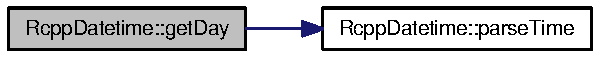
\includegraphics[width=162pt]{classRcppDatetime_23e9f09bef162e1ffef0e43f8a446b77_cgraph}
\end{center}
\end{figure}
\hypertarget{classRcppDatetime_cb74d27387c0d851414e20d30354ac62}{
\index{RcppDatetime@{RcppDatetime}!getFractionalTimestamp@{getFractionalTimestamp}}
\index{getFractionalTimestamp@{getFractionalTimestamp}!RcppDatetime@{RcppDatetime}}
\subsubsection[{getFractionalTimestamp}]{\setlength{\rightskip}{0pt plus 5cm}double RcppDatetime::getFractionalTimestamp (void) const\hspace{0.3cm}{\tt  \mbox{[}inline\mbox{]}}}}
\label{classRcppDatetime_cb74d27387c0d851414e20d30354ac62}




Definition at line 114 of file Rcpp.h.

References m\_\-d.

Referenced by RcppResultSet::add(), and RcppFunction::appendToRList().\hypertarget{classRcppDatetime_0da8db1ecd235a6e7ab309e70e4e93b0}{
\index{RcppDatetime@{RcppDatetime}!getHour@{getHour}}
\index{getHour@{getHour}!RcppDatetime@{RcppDatetime}}
\subsubsection[{getHour}]{\setlength{\rightskip}{0pt plus 5cm}int RcppDatetime::getHour (void)\hspace{0.3cm}{\tt  \mbox{[}inline\mbox{]}}}}
\label{classRcppDatetime_0da8db1ecd235a6e7ab309e70e4e93b0}




Definition at line 120 of file Rcpp.h.

References m\_\-parsed, m\_\-tm, and parseTime().

Here is the call graph for this function:\nopagebreak
\begin{figure}[H]
\begin{center}
\leavevmode
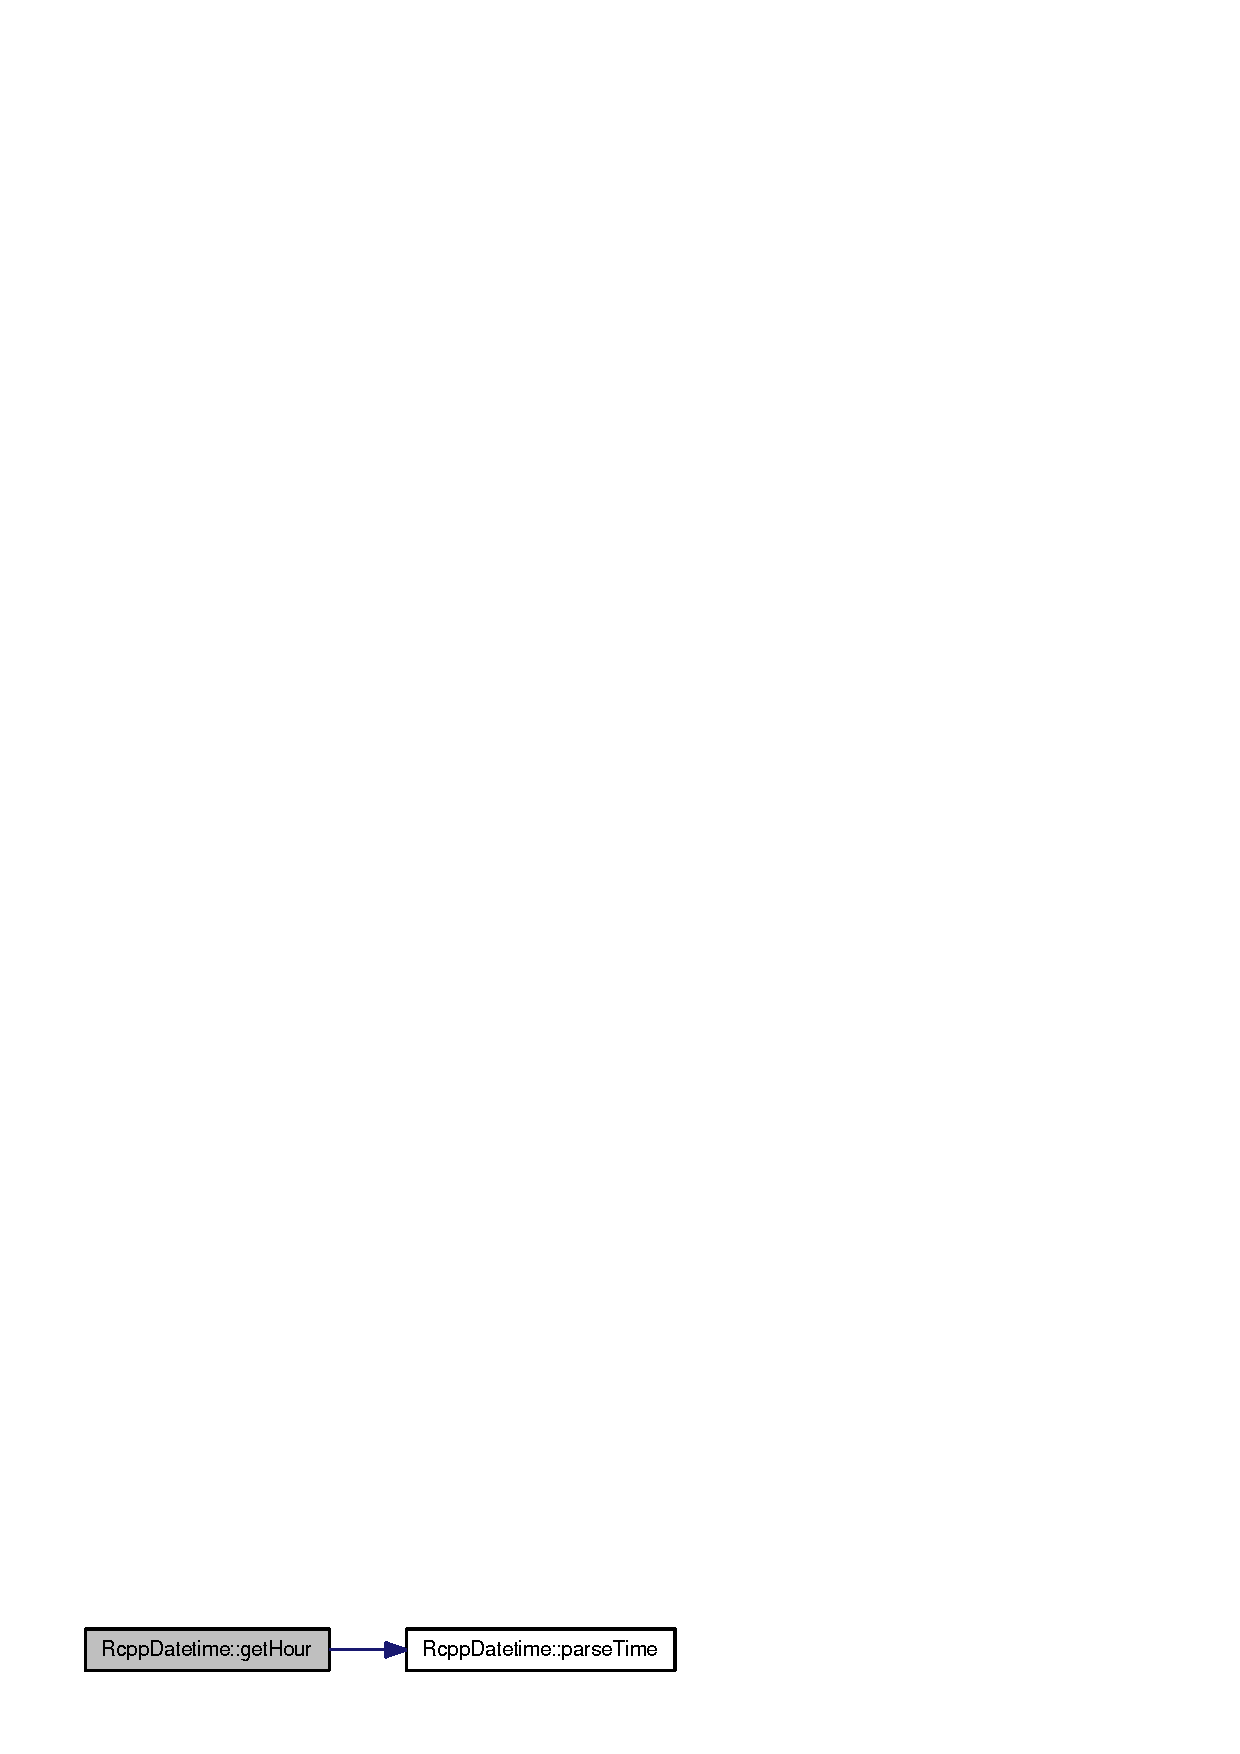
\includegraphics[width=164pt]{classRcppDatetime_0da8db1ecd235a6e7ab309e70e4e93b0_cgraph}
\end{center}
\end{figure}
\hypertarget{classRcppDatetime_cdf9e19f28c84fde38c352df5f225999}{
\index{RcppDatetime@{RcppDatetime}!getMicroSec@{getMicroSec}}
\index{getMicroSec@{getMicroSec}!RcppDatetime@{RcppDatetime}}
\subsubsection[{getMicroSec}]{\setlength{\rightskip}{0pt plus 5cm}int RcppDatetime::getMicroSec (void)\hspace{0.3cm}{\tt  \mbox{[}inline\mbox{]}}}}
\label{classRcppDatetime_cdf9e19f28c84fde38c352df5f225999}




Definition at line 123 of file Rcpp.h.

References m\_\-parsed, m\_\-us, and parseTime().

Here is the call graph for this function:\nopagebreak
\begin{figure}[H]
\begin{center}
\leavevmode
\includegraphics[width=174pt]{classRcppDatetime_cdf9e19f28c84fde38c352df5f225999_cgraph}
\end{center}
\end{figure}
\hypertarget{classRcppDatetime_db41bd524ead66d69e129b1f2767358a}{
\index{RcppDatetime@{RcppDatetime}!getMinute@{getMinute}}
\index{getMinute@{getMinute}!RcppDatetime@{RcppDatetime}}
\subsubsection[{getMinute}]{\setlength{\rightskip}{0pt plus 5cm}int RcppDatetime::getMinute (void)\hspace{0.3cm}{\tt  \mbox{[}inline\mbox{]}}}}
\label{classRcppDatetime_db41bd524ead66d69e129b1f2767358a}




Definition at line 121 of file Rcpp.h.

References m\_\-parsed, m\_\-tm, and parseTime().

Here is the call graph for this function:\nopagebreak
\begin{figure}[H]
\begin{center}
\leavevmode
\includegraphics[width=168pt]{classRcppDatetime_db41bd524ead66d69e129b1f2767358a_cgraph}
\end{center}
\end{figure}
\hypertarget{classRcppDatetime_a7f04947d2a27e4bba2d19efa21771ed}{
\index{RcppDatetime@{RcppDatetime}!getMonth@{getMonth}}
\index{getMonth@{getMonth}!RcppDatetime@{RcppDatetime}}
\subsubsection[{getMonth}]{\setlength{\rightskip}{0pt plus 5cm}int RcppDatetime::getMonth (void)\hspace{0.3cm}{\tt  \mbox{[}inline\mbox{]}}}}
\label{classRcppDatetime_a7f04947d2a27e4bba2d19efa21771ed}




Definition at line 117 of file Rcpp.h.

References m\_\-parsed, m\_\-tm, and parseTime().

Here is the call graph for this function:\nopagebreak
\begin{figure}[H]
\begin{center}
\leavevmode
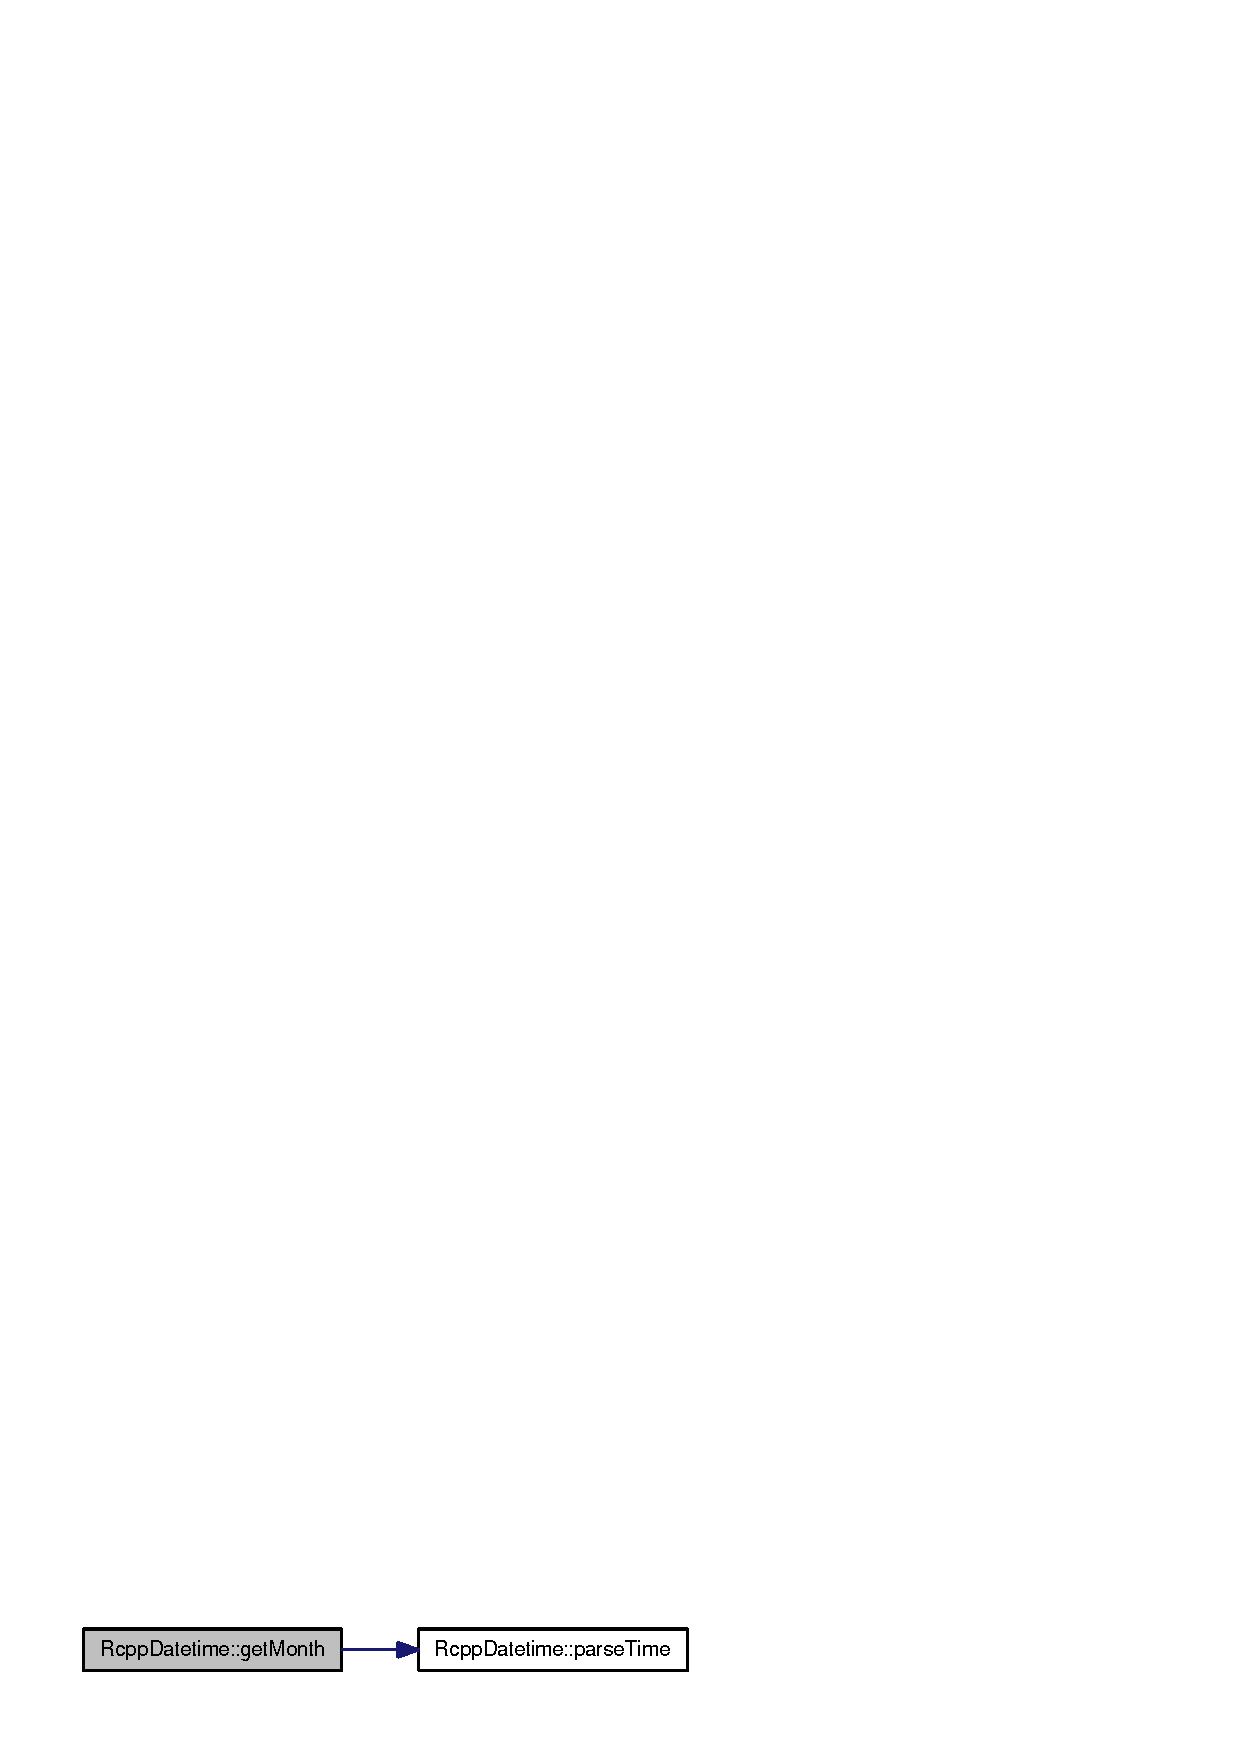
\includegraphics[width=167pt]{classRcppDatetime_a7f04947d2a27e4bba2d19efa21771ed_cgraph}
\end{center}
\end{figure}
\hypertarget{classRcppDatetime_2feb900005890d183cc5f6a626c4d614}{
\index{RcppDatetime@{RcppDatetime}!getSecond@{getSecond}}
\index{getSecond@{getSecond}!RcppDatetime@{RcppDatetime}}
\subsubsection[{getSecond}]{\setlength{\rightskip}{0pt plus 5cm}int RcppDatetime::getSecond (void)\hspace{0.3cm}{\tt  \mbox{[}inline\mbox{]}}}}
\label{classRcppDatetime_2feb900005890d183cc5f6a626c4d614}




Definition at line 122 of file Rcpp.h.

References m\_\-parsed, m\_\-tm, and parseTime().

Here is the call graph for this function:\nopagebreak
\begin{figure}[H]
\begin{center}
\leavevmode
\includegraphics[width=170pt]{classRcppDatetime_2feb900005890d183cc5f6a626c4d614_cgraph}
\end{center}
\end{figure}
\hypertarget{classRcppDatetime_796802561fa8bb87a8e2a1836afaaa58}{
\index{RcppDatetime@{RcppDatetime}!getWeekday@{getWeekday}}
\index{getWeekday@{getWeekday}!RcppDatetime@{RcppDatetime}}
\subsubsection[{getWeekday}]{\setlength{\rightskip}{0pt plus 5cm}int RcppDatetime::getWeekday (void)\hspace{0.3cm}{\tt  \mbox{[}inline\mbox{]}}}}
\label{classRcppDatetime_796802561fa8bb87a8e2a1836afaaa58}




Definition at line 119 of file Rcpp.h.

References m\_\-parsed, m\_\-tm, and parseTime().

Here is the call graph for this function:\nopagebreak
\begin{figure}[H]
\begin{center}
\leavevmode
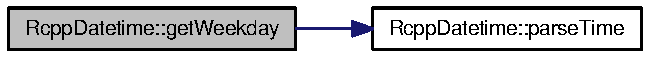
\includegraphics[width=174pt]{classRcppDatetime_796802561fa8bb87a8e2a1836afaaa58_cgraph}
\end{center}
\end{figure}
\hypertarget{classRcppDatetime_ba930a8d7d575eb10444258a442027cf}{
\index{RcppDatetime@{RcppDatetime}!getYear@{getYear}}
\index{getYear@{getYear}!RcppDatetime@{RcppDatetime}}
\subsubsection[{getYear}]{\setlength{\rightskip}{0pt plus 5cm}int RcppDatetime::getYear (void)\hspace{0.3cm}{\tt  \mbox{[}inline\mbox{]}}}}
\label{classRcppDatetime_ba930a8d7d575eb10444258a442027cf}




Definition at line 116 of file Rcpp.h.

References m\_\-parsed, m\_\-tm, and parseTime().

Here is the call graph for this function:\nopagebreak
\begin{figure}[H]
\begin{center}
\leavevmode
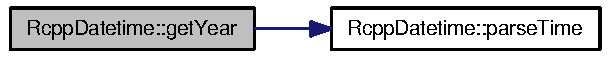
\includegraphics[width=164pt]{classRcppDatetime_ba930a8d7d575eb10444258a442027cf_cgraph}
\end{center}
\end{figure}
\hypertarget{classRcppDatetime_a4b2eba45c4c02b5d334dd89e080b660}{
\index{RcppDatetime@{RcppDatetime}!parseTime@{parseTime}}
\index{parseTime@{parseTime}!RcppDatetime@{RcppDatetime}}
\subsubsection[{parseTime}]{\setlength{\rightskip}{0pt plus 5cm}void RcppDatetime::parseTime ()\hspace{0.3cm}{\tt  \mbox{[}inline, private\mbox{]}}}}
\label{classRcppDatetime_a4b2eba45c4c02b5d334dd89e080b660}




Definition at line 96 of file Rcpp.h.

References m\_\-d, m\_\-parsed, m\_\-tm, and m\_\-us.

Referenced by getDay(), getHour(), getMicroSec(), getMinute(), getMonth(), getSecond(), getWeekday(), and getYear().

\subsection{Friends And Related Function Documentation}
\hypertarget{classRcppDatetime_2740dcf7de2c2f5471d8fa18944a98d7}{
\index{RcppDatetime@{RcppDatetime}!ColDatum@{ColDatum}}
\index{ColDatum@{ColDatum}!RcppDatetime@{RcppDatetime}}
\subsubsection[{ColDatum}]{\setlength{\rightskip}{0pt plus 5cm}friend class {\bf ColDatum}\hspace{0.3cm}{\tt  \mbox{[}friend\mbox{]}}}}
\label{classRcppDatetime_2740dcf7de2c2f5471d8fa18944a98d7}




Definition at line 103 of file Rcpp.h.\hypertarget{classRcppDatetime_29513e04f8cb90b2a7efea97f8cbd37a}{
\index{RcppDatetime@{RcppDatetime}!operator+@{operator+}}
\index{operator+@{operator+}!RcppDatetime@{RcppDatetime}}
\subsubsection[{operator+}]{\setlength{\rightskip}{0pt plus 5cm}{\bf RcppDatetime} operator+ (const {\bf RcppDatetime} \& {\em date}, \/  double {\em offset})\hspace{0.3cm}{\tt  \mbox{[}friend\mbox{]}}}}
\label{classRcppDatetime_29513e04f8cb90b2a7efea97f8cbd37a}




Definition at line 125 of file Rcpp.h.\hypertarget{classRcppDatetime_946df17f9ce3c423518d0db74e2bbbc4}{
\index{RcppDatetime@{RcppDatetime}!operator-@{operator-}}
\index{operator-@{operator-}!RcppDatetime@{RcppDatetime}}
\subsubsection[{operator-}]{\setlength{\rightskip}{0pt plus 5cm}double operator- (const {\bf RcppDatetime} \& {\em dt1}, \/  const {\bf RcppDatetime} \& {\em dt2})\hspace{0.3cm}{\tt  \mbox{[}friend\mbox{]}}}}
\label{classRcppDatetime_946df17f9ce3c423518d0db74e2bbbc4}




Definition at line 131 of file Rcpp.h.\hypertarget{classRcppDatetime_142f9346629bf7a6f673ba05d9338cf3}{
\index{RcppDatetime@{RcppDatetime}!operator$<$@{operator$<$}}
\index{operator$<$@{operator$<$}!RcppDatetime@{RcppDatetime}}
\subsubsection[{operator$<$}]{\setlength{\rightskip}{0pt plus 5cm}bool operator$<$ (const {\bf RcppDatetime} \& {\em dt1}, \/  const {\bf RcppDatetime} \& {\em dt2})\hspace{0.3cm}{\tt  \mbox{[}friend\mbox{]}}}}
\label{classRcppDatetime_142f9346629bf7a6f673ba05d9338cf3}




Definition at line 132 of file Rcpp.h.\hypertarget{classRcppDatetime_778b21a52b7f2b17978933c3ec27754e}{
\index{RcppDatetime@{RcppDatetime}!operator$<$$<$@{operator$<$$<$}}
\index{operator$<$$<$@{operator$<$$<$}!RcppDatetime@{RcppDatetime}}
\subsubsection[{operator$<$$<$}]{\setlength{\rightskip}{0pt plus 5cm}std::ostream\& operator$<$$<$ (std::ostream \& {\em os}, \/  const {\bf RcppDatetime} \& {\em datetime})\hspace{0.3cm}{\tt  \mbox{[}friend\mbox{]}}}}
\label{classRcppDatetime_778b21a52b7f2b17978933c3ec27754e}




Definition at line 138 of file Rcpp.h.\hypertarget{classRcppDatetime_7d98733f95f5647ac10bb8236c1a7a8d}{
\index{RcppDatetime@{RcppDatetime}!operator$<$=@{operator$<$=}}
\index{operator$<$=@{operator$<$=}!RcppDatetime@{RcppDatetime}}
\subsubsection[{operator$<$=}]{\setlength{\rightskip}{0pt plus 5cm}bool operator$<$= (const {\bf RcppDatetime} \& {\em dt1}, \/  const {\bf RcppDatetime} \& {\em dt2})\hspace{0.3cm}{\tt  \mbox{[}friend\mbox{]}}}}
\label{classRcppDatetime_7d98733f95f5647ac10bb8236c1a7a8d}




Definition at line 133 of file Rcpp.h.\hypertarget{classRcppDatetime_c6643666732e0a62c501da9f0ae9e342}{
\index{RcppDatetime@{RcppDatetime}!operator==@{operator==}}
\index{operator==@{operator==}!RcppDatetime@{RcppDatetime}}
\subsubsection[{operator==}]{\setlength{\rightskip}{0pt plus 5cm}bool operator== (const {\bf RcppDatetime} \& {\em dt1}, \/  const {\bf RcppDatetime} \& {\em dt2})\hspace{0.3cm}{\tt  \mbox{[}friend\mbox{]}}}}
\label{classRcppDatetime_c6643666732e0a62c501da9f0ae9e342}




Definition at line 136 of file Rcpp.h.\hypertarget{classRcppDatetime_062107b2e2809a60c67f80da5dab77ed}{
\index{RcppDatetime@{RcppDatetime}!operator$>$@{operator$>$}}
\index{operator$>$@{operator$>$}!RcppDatetime@{RcppDatetime}}
\subsubsection[{operator$>$}]{\setlength{\rightskip}{0pt plus 5cm}bool operator$>$ (const {\bf RcppDatetime} \& {\em dt1}, \/  const {\bf RcppDatetime} \& {\em dt2})\hspace{0.3cm}{\tt  \mbox{[}friend\mbox{]}}}}
\label{classRcppDatetime_062107b2e2809a60c67f80da5dab77ed}




Definition at line 134 of file Rcpp.h.\hypertarget{classRcppDatetime_1aac48969216af0555677a43b3617781}{
\index{RcppDatetime@{RcppDatetime}!operator$>$=@{operator$>$=}}
\index{operator$>$=@{operator$>$=}!RcppDatetime@{RcppDatetime}}
\subsubsection[{operator$>$=}]{\setlength{\rightskip}{0pt plus 5cm}bool operator$>$= (const {\bf RcppDatetime} \& {\em dt1}, \/  const {\bf RcppDatetime} \& {\em dt2})\hspace{0.3cm}{\tt  \mbox{[}friend\mbox{]}}}}
\label{classRcppDatetime_1aac48969216af0555677a43b3617781}




Definition at line 135 of file Rcpp.h.

\subsection{Member Data Documentation}
\hypertarget{classRcppDatetime_1af187ff381bfa0f5b57d28b64d7b60c}{
\index{RcppDatetime@{RcppDatetime}!m\_\-d@{m\_\-d}}
\index{m\_\-d@{m\_\-d}!RcppDatetime@{RcppDatetime}}
\subsubsection[{m\_\-d}]{\setlength{\rightskip}{0pt plus 5cm}double {\bf RcppDatetime::m\_\-d}\hspace{0.3cm}{\tt  \mbox{[}private\mbox{]}}}}
\label{classRcppDatetime_1af187ff381bfa0f5b57d28b64d7b60c}




Definition at line 92 of file Rcpp.h.

Referenced by getFractionalTimestamp(), parseTime(), and ColDatum::setDatetimeValue().\hypertarget{classRcppDatetime_515e3390c1834e58ce6bba39854638ad}{
\index{RcppDatetime@{RcppDatetime}!m\_\-parsed@{m\_\-parsed}}
\index{m\_\-parsed@{m\_\-parsed}!RcppDatetime@{RcppDatetime}}
\subsubsection[{m\_\-parsed}]{\setlength{\rightskip}{0pt plus 5cm}bool {\bf RcppDatetime::m\_\-parsed}\hspace{0.3cm}{\tt  \mbox{[}private\mbox{]}}}}
\label{classRcppDatetime_515e3390c1834e58ce6bba39854638ad}




Definition at line 93 of file Rcpp.h.

Referenced by getDay(), getHour(), getMicroSec(), getMinute(), getMonth(), getSecond(), getWeekday(), getYear(), and parseTime().\hypertarget{classRcppDatetime_3f65c708657270208656c1be885e9f1b}{
\index{RcppDatetime@{RcppDatetime}!m\_\-tm@{m\_\-tm}}
\index{m\_\-tm@{m\_\-tm}!RcppDatetime@{RcppDatetime}}
\subsubsection[{m\_\-tm}]{\setlength{\rightskip}{0pt plus 5cm}struct tm {\bf RcppDatetime::m\_\-tm}\hspace{0.3cm}{\tt  \mbox{[}read, private\mbox{]}}}}
\label{classRcppDatetime_3f65c708657270208656c1be885e9f1b}




Definition at line 95 of file Rcpp.h.

Referenced by getDay(), getHour(), getMinute(), getMonth(), getSecond(), getWeekday(), getYear(), and parseTime().\hypertarget{classRcppDatetime_68b9c7b759ffbba14aca3ae0680ea8a4}{
\index{RcppDatetime@{RcppDatetime}!m\_\-us@{m\_\-us}}
\index{m\_\-us@{m\_\-us}!RcppDatetime@{RcppDatetime}}
\subsubsection[{m\_\-us}]{\setlength{\rightskip}{0pt plus 5cm}int {\bf RcppDatetime::m\_\-us}\hspace{0.3cm}{\tt  \mbox{[}private\mbox{]}}}}
\label{classRcppDatetime_68b9c7b759ffbba14aca3ae0680ea8a4}




Definition at line 94 of file Rcpp.h.

Referenced by getMicroSec(), and parseTime().

The documentation for this class was generated from the following file:\begin{CompactItemize}
\item 
src/\hyperlink{Rcpp_8h}{Rcpp.h}\end{CompactItemize}

\hypertarget{classRcppDatetimeVector}{
\section{RcppDatetimeVector Class Reference}
\label{classRcppDatetimeVector}\index{RcppDatetimeVector@{RcppDatetimeVector}}
}
{\tt \#include $<$Rcpp.h$>$}

Collaboration diagram for RcppDatetimeVector:\nopagebreak
\begin{figure}[H]
\begin{center}
\leavevmode
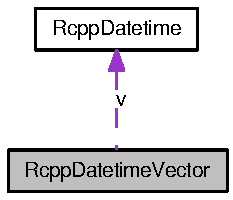
\includegraphics[width=75pt]{classRcppDatetimeVector__coll__graph}
\end{center}
\end{figure}
\subsection*{Public Member Functions}
\begin{CompactItemize}
\item 
\hyperlink{classRcppDatetimeVector_1c1d1e2087fdc8e7601299dc2c4fe24c}{RcppDatetimeVector} (SEXP vec)
\item 
\hyperlink{classRcppDatetimeVector_81d6c5daba7448058a2f896841ddeb3a}{$\sim$RcppDatetimeVector} ()
\item 
\hyperlink{classRcppDatetime}{RcppDatetime} \& \hyperlink{classRcppDatetimeVector_2ffa33b5231a7975652e1e2498d0e16a}{operator()} (int i)
\item 
int \hyperlink{classRcppDatetimeVector_8ca7268098fb2b9250523c4e2ef3c8b7}{size} ()
\end{CompactItemize}
\subsection*{Private Attributes}
\begin{CompactItemize}
\item 
\hyperlink{classRcppDatetime}{RcppDatetime} $\ast$ \hyperlink{classRcppDatetimeVector_0138476000351892e9ec591b2c9ec02f}{v}
\item 
int \hyperlink{classRcppDatetimeVector_e131031fcf2e65b7bfeee3d8e25c4f8c}{length}
\end{CompactItemize}


\subsection{Detailed Description}


Definition at line 424 of file Rcpp.h.

\subsection{Constructor \& Destructor Documentation}
\hypertarget{classRcppDatetimeVector_1c1d1e2087fdc8e7601299dc2c4fe24c}{
\index{RcppDatetimeVector@{RcppDatetimeVector}!RcppDatetimeVector@{RcppDatetimeVector}}
\index{RcppDatetimeVector@{RcppDatetimeVector}!RcppDatetimeVector@{RcppDatetimeVector}}
\subsubsection[RcppDatetimeVector]{\setlength{\rightskip}{0pt plus 5cm}RcppDatetimeVector::RcppDatetimeVector (SEXP {\em vec})}}
\label{classRcppDatetimeVector_1c1d1e2087fdc8e7601299dc2c4fe24c}




Definition at line 261 of file Rcpp.cpp.

References length, and v.\hypertarget{classRcppDatetimeVector_81d6c5daba7448058a2f896841ddeb3a}{
\index{RcppDatetimeVector@{RcppDatetimeVector}!$\sim$RcppDatetimeVector@{$\sim$RcppDatetimeVector}}
\index{$\sim$RcppDatetimeVector@{$\sim$RcppDatetimeVector}!RcppDatetimeVector@{RcppDatetimeVector}}
\subsubsection[$\sim$RcppDatetimeVector]{\setlength{\rightskip}{0pt plus 5cm}RcppDatetimeVector::$\sim$RcppDatetimeVector ()\hspace{0.3cm}{\tt  \mbox{[}inline\mbox{]}}}}
\label{classRcppDatetimeVector_81d6c5daba7448058a2f896841ddeb3a}




Definition at line 427 of file Rcpp.h.

References v.

\subsection{Member Function Documentation}
\hypertarget{classRcppDatetimeVector_2ffa33b5231a7975652e1e2498d0e16a}{
\index{RcppDatetimeVector@{RcppDatetimeVector}!operator()@{operator()}}
\index{operator()@{operator()}!RcppDatetimeVector@{RcppDatetimeVector}}
\subsubsection[operator()]{\setlength{\rightskip}{0pt plus 5cm}{\bf RcppDatetime}\& RcppDatetimeVector::operator() (int {\em i})\hspace{0.3cm}{\tt  \mbox{[}inline\mbox{]}}}}
\label{classRcppDatetimeVector_2ffa33b5231a7975652e1e2498d0e16a}




Definition at line 430 of file Rcpp.h.

References length, and v.\hypertarget{classRcppDatetimeVector_8ca7268098fb2b9250523c4e2ef3c8b7}{
\index{RcppDatetimeVector@{RcppDatetimeVector}!size@{size}}
\index{size@{size}!RcppDatetimeVector@{RcppDatetimeVector}}
\subsubsection[size]{\setlength{\rightskip}{0pt plus 5cm}int RcppDatetimeVector::size ()\hspace{0.3cm}{\tt  \mbox{[}inline\mbox{]}}}}
\label{classRcppDatetimeVector_8ca7268098fb2b9250523c4e2ef3c8b7}




Definition at line 438 of file Rcpp.h.

References length.

Referenced by RcppResultSet::add(), and RcppDateExample().

\subsection{Member Data Documentation}
\hypertarget{classRcppDatetimeVector_0138476000351892e9ec591b2c9ec02f}{
\index{RcppDatetimeVector@{RcppDatetimeVector}!v@{v}}
\index{v@{v}!RcppDatetimeVector@{RcppDatetimeVector}}
\subsubsection[v]{\setlength{\rightskip}{0pt plus 5cm}{\bf RcppDatetime}$\ast$ {\bf RcppDatetimeVector::v}\hspace{0.3cm}{\tt  \mbox{[}private\mbox{]}}}}
\label{classRcppDatetimeVector_0138476000351892e9ec591b2c9ec02f}




Definition at line 440 of file Rcpp.h.

Referenced by operator()(), RcppDatetimeVector(), and $\sim$RcppDatetimeVector().\hypertarget{classRcppDatetimeVector_e131031fcf2e65b7bfeee3d8e25c4f8c}{
\index{RcppDatetimeVector@{RcppDatetimeVector}!length@{length}}
\index{length@{length}!RcppDatetimeVector@{RcppDatetimeVector}}
\subsubsection[length]{\setlength{\rightskip}{0pt plus 5cm}int {\bf RcppDatetimeVector::length}\hspace{0.3cm}{\tt  \mbox{[}private\mbox{]}}}}
\label{classRcppDatetimeVector_e131031fcf2e65b7bfeee3d8e25c4f8c}




Definition at line 441 of file Rcpp.h.

Referenced by operator()(), RcppDatetimeVector(), and size().

The documentation for this class was generated from the following files:\begin{CompactItemize}
\item 
src/\hyperlink{Rcpp_8h}{Rcpp.h}\item 
src/\hyperlink{Rcpp_8cpp}{Rcpp.cpp}\end{CompactItemize}

\hypertarget{classRcppDateVector}{
\section{RcppDateVector Class Reference}
\label{classRcppDateVector}\index{RcppDateVector@{RcppDateVector}}
}
{\tt \#include $<$Rcpp.h$>$}

Collaboration diagram for RcppDateVector:\nopagebreak
\begin{figure}[H]
\begin{center}
\leavevmode
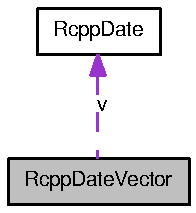
\includegraphics[width=130pt]{classRcppDateVector__coll__graph}
\end{center}
\end{figure}
\subsection*{Public Member Functions}
\begin{CompactItemize}
\item 
\hyperlink{classRcppDateVector_65de4c0807f5c4b33429c8ebb5224831}{RcppDateVector} (SEXP vec)
\item 
\hyperlink{classRcppDateVector_ad0851f7555a09615ccb17bcb20fc7f1}{$\sim$RcppDateVector} ()
\item 
\hyperlink{classRcppDate}{RcppDate} \& \hyperlink{classRcppDateVector_7a6d9ceb233ed06f037013bdf4088a23}{operator()} (int i)
\item 
int \hyperlink{classRcppDateVector_03db4282da968eb4e0ae2a38375e0d37}{size} ()
\end{CompactItemize}
\subsection*{Private Attributes}
\begin{CompactItemize}
\item 
\hyperlink{classRcppDate}{RcppDate} $\ast$ \hyperlink{classRcppDateVector_faa34ebaf3d8bac309e81895c376f545}{v}
\item 
int \hyperlink{classRcppDateVector_a36764f68111a84b737b78600ff06433}{length}
\end{CompactItemize}


\subsection{Detailed Description}


Definition at line 405 of file Rcpp.h.

\subsection{Constructor \& Destructor Documentation}
\hypertarget{classRcppDateVector_65de4c0807f5c4b33429c8ebb5224831}{
\index{RcppDateVector@{RcppDateVector}!RcppDateVector@{RcppDateVector}}
\index{RcppDateVector@{RcppDateVector}!RcppDateVector@{RcppDateVector}}
\subsubsection[{RcppDateVector}]{\setlength{\rightskip}{0pt plus 5cm}RcppDateVector::RcppDateVector (SEXP {\em vec})}}
\label{classRcppDateVector_65de4c0807f5c4b33429c8ebb5224831}




Definition at line 257 of file Rcpp.cpp.

References length, and v.\hypertarget{classRcppDateVector_ad0851f7555a09615ccb17bcb20fc7f1}{
\index{RcppDateVector@{RcppDateVector}!$\sim$RcppDateVector@{$\sim$RcppDateVector}}
\index{$\sim$RcppDateVector@{$\sim$RcppDateVector}!RcppDateVector@{RcppDateVector}}
\subsubsection[{$\sim$RcppDateVector}]{\setlength{\rightskip}{0pt plus 5cm}RcppDateVector::$\sim$RcppDateVector ()\hspace{0.3cm}{\tt  \mbox{[}inline\mbox{]}}}}
\label{classRcppDateVector_ad0851f7555a09615ccb17bcb20fc7f1}




Definition at line 408 of file Rcpp.h.

References v.

\subsection{Member Function Documentation}
\hypertarget{classRcppDateVector_7a6d9ceb233ed06f037013bdf4088a23}{
\index{RcppDateVector@{RcppDateVector}!operator()@{operator()}}
\index{operator()@{operator()}!RcppDateVector@{RcppDateVector}}
\subsubsection[{operator()}]{\setlength{\rightskip}{0pt plus 5cm}{\bf RcppDate}\& RcppDateVector::operator() (int {\em i})\hspace{0.3cm}{\tt  \mbox{[}inline\mbox{]}}}}
\label{classRcppDateVector_7a6d9ceb233ed06f037013bdf4088a23}




Definition at line 411 of file Rcpp.h.

References length, and v.\hypertarget{classRcppDateVector_03db4282da968eb4e0ae2a38375e0d37}{
\index{RcppDateVector@{RcppDateVector}!size@{size}}
\index{size@{size}!RcppDateVector@{RcppDateVector}}
\subsubsection[{size}]{\setlength{\rightskip}{0pt plus 5cm}int RcppDateVector::size ()\hspace{0.3cm}{\tt  \mbox{[}inline\mbox{]}}}}
\label{classRcppDateVector_03db4282da968eb4e0ae2a38375e0d37}




Definition at line 419 of file Rcpp.h.

References length.

Referenced by RcppResultSet::add(), and RcppDateExample().

\subsection{Member Data Documentation}
\hypertarget{classRcppDateVector_a36764f68111a84b737b78600ff06433}{
\index{RcppDateVector@{RcppDateVector}!length@{length}}
\index{length@{length}!RcppDateVector@{RcppDateVector}}
\subsubsection[{length}]{\setlength{\rightskip}{0pt plus 5cm}int {\bf RcppDateVector::length}\hspace{0.3cm}{\tt  \mbox{[}private\mbox{]}}}}
\label{classRcppDateVector_a36764f68111a84b737b78600ff06433}




Definition at line 422 of file Rcpp.h.

Referenced by operator()(), RcppDateVector(), and size().\hypertarget{classRcppDateVector_faa34ebaf3d8bac309e81895c376f545}{
\index{RcppDateVector@{RcppDateVector}!v@{v}}
\index{v@{v}!RcppDateVector@{RcppDateVector}}
\subsubsection[{v}]{\setlength{\rightskip}{0pt plus 5cm}{\bf RcppDate}$\ast$ {\bf RcppDateVector::v}\hspace{0.3cm}{\tt  \mbox{[}private\mbox{]}}}}
\label{classRcppDateVector_faa34ebaf3d8bac309e81895c376f545}




Definition at line 421 of file Rcpp.h.

Referenced by operator()(), RcppDateVector(), and $\sim$RcppDateVector().

The documentation for this class was generated from the following files:\begin{CompactItemize}
\item 
src/\hyperlink{Rcpp_8h}{Rcpp.h}\item 
src/\hyperlink{Rcpp_8cpp}{Rcpp.cpp}\end{CompactItemize}

\hypertarget{classRcppFrame}{
\section{RcppFrame Class Reference}
\label{classRcppFrame}\index{RcppFrame@{RcppFrame}}
}
{\tt \#include $<$Rcpp.h$>$}

\subsection*{Public Member Functions}
\begin{CompactItemize}
\item 
\hyperlink{classRcppFrame_2aad548eb7d3842ea12da3c5a67bbfbc}{RcppFrame} (SEXP df)
\item 
\hyperlink{classRcppFrame_d3caf84a0543c0f31a97705be8902358}{RcppFrame} (std::vector$<$ std::string $>$ \hyperlink{classRcppFrame_9b549d377248896848b6abcb8df64f82}{colNames})
\item 
std::vector$<$ std::string $>$ \& \hyperlink{classRcppFrame_d220bfd289e745d13a99ffe323a00200}{getColNames} ()
\item 
std::vector$<$ std::vector$<$ \hyperlink{classColDatum}{ColDatum} $>$ $>$ \& \hyperlink{classRcppFrame_3a0ac7b2822fc590f6f93ee775b134d0}{getTableData} ()
\item 
void \hyperlink{classRcppFrame_ae72791527f2947a477633151106f42c}{addRow} (std::vector$<$ \hyperlink{classColDatum}{ColDatum} $>$ rowData)
\item 
int \hyperlink{classRcppFrame_a33ab9553bb9fa510c338a3e092d9ace}{rows} ()
\item 
int \hyperlink{classRcppFrame_ac33f787068fe1bc6f97b2b4e08c9c5d}{cols} ()
\end{CompactItemize}
\subsection*{Private Attributes}
\begin{CompactItemize}
\item 
std::vector$<$ std::string $>$ \hyperlink{classRcppFrame_9b549d377248896848b6abcb8df64f82}{colNames}
\item 
std::vector$<$ std::vector$<$ \hyperlink{classColDatum}{ColDatum} $>$ $>$ \hyperlink{classRcppFrame_4de0bda5c0df650b2447a4c029af0302}{table}
\end{CompactItemize}


\subsection{Detailed Description}


Definition at line 286 of file Rcpp.h.

\subsection{Constructor \& Destructor Documentation}
\hypertarget{classRcppFrame_2aad548eb7d3842ea12da3c5a67bbfbc}{
\index{RcppFrame@{RcppFrame}!RcppFrame@{RcppFrame}}
\index{RcppFrame@{RcppFrame}!RcppFrame@{RcppFrame}}
\subsubsection[{RcppFrame}]{\setlength{\rightskip}{0pt plus 5cm}RcppFrame::RcppFrame (SEXP {\em df})}}
\label{classRcppFrame_2aad548eb7d3842ea12da3c5a67bbfbc}




Definition at line 59 of file Rcpp.cpp.

References colNames, and table.\hypertarget{classRcppFrame_d3caf84a0543c0f31a97705be8902358}{
\index{RcppFrame@{RcppFrame}!RcppFrame@{RcppFrame}}
\index{RcppFrame@{RcppFrame}!RcppFrame@{RcppFrame}}
\subsubsection[{RcppFrame}]{\setlength{\rightskip}{0pt plus 5cm}RcppFrame::RcppFrame (std::vector$<$ std::string $>$ {\em colNames})\hspace{0.3cm}{\tt  \mbox{[}inline\mbox{]}}}}
\label{classRcppFrame_d3caf84a0543c0f31a97705be8902358}




Definition at line 291 of file Rcpp.h.

\subsection{Member Function Documentation}
\hypertarget{classRcppFrame_ae72791527f2947a477633151106f42c}{
\index{RcppFrame@{RcppFrame}!addRow@{addRow}}
\index{addRow@{addRow}!RcppFrame@{RcppFrame}}
\subsubsection[{addRow}]{\setlength{\rightskip}{0pt plus 5cm}void RcppFrame::addRow (std::vector$<$ {\bf ColDatum} $>$ {\em rowData})\hspace{0.3cm}{\tt  \mbox{[}inline\mbox{]}}}}
\label{classRcppFrame_ae72791527f2947a477633151106f42c}




Definition at line 297 of file Rcpp.h.

References colNames, and table.

Referenced by Rcpp\_\-Example().\hypertarget{classRcppFrame_ac33f787068fe1bc6f97b2b4e08c9c5d}{
\index{RcppFrame@{RcppFrame}!cols@{cols}}
\index{cols@{cols}!RcppFrame@{RcppFrame}}
\subsubsection[{cols}]{\setlength{\rightskip}{0pt plus 5cm}int RcppFrame::cols ()\hspace{0.3cm}{\tt  \mbox{[}inline\mbox{]}}}}
\label{classRcppFrame_ac33f787068fe1bc6f97b2b4e08c9c5d}




Definition at line 316 of file Rcpp.h.

References table.\hypertarget{classRcppFrame_d220bfd289e745d13a99ffe323a00200}{
\index{RcppFrame@{RcppFrame}!getColNames@{getColNames}}
\index{getColNames@{getColNames}!RcppFrame@{RcppFrame}}
\subsubsection[{getColNames}]{\setlength{\rightskip}{0pt plus 5cm}std::vector$<$std::string$>$\& RcppFrame::getColNames ()\hspace{0.3cm}{\tt  \mbox{[}inline\mbox{]}}}}
\label{classRcppFrame_d220bfd289e745d13a99ffe323a00200}




Definition at line 295 of file Rcpp.h.

References colNames.

Referenced by RcppResultSet::add().\hypertarget{classRcppFrame_3a0ac7b2822fc590f6f93ee775b134d0}{
\index{RcppFrame@{RcppFrame}!getTableData@{getTableData}}
\index{getTableData@{getTableData}!RcppFrame@{RcppFrame}}
\subsubsection[{getTableData}]{\setlength{\rightskip}{0pt plus 5cm}std::vector$<$std::vector$<${\bf ColDatum}$>$ $>$\& RcppFrame::getTableData ()\hspace{0.3cm}{\tt  \mbox{[}inline\mbox{]}}}}
\label{classRcppFrame_3a0ac7b2822fc590f6f93ee775b134d0}




Definition at line 296 of file Rcpp.h.

References table.

Referenced by RcppResultSet::add().\hypertarget{classRcppFrame_a33ab9553bb9fa510c338a3e092d9ace}{
\index{RcppFrame@{RcppFrame}!rows@{rows}}
\index{rows@{rows}!RcppFrame@{RcppFrame}}
\subsubsection[{rows}]{\setlength{\rightskip}{0pt plus 5cm}int RcppFrame::rows ()\hspace{0.3cm}{\tt  \mbox{[}inline\mbox{]}}}}
\label{classRcppFrame_a33ab9553bb9fa510c338a3e092d9ace}




Definition at line 315 of file Rcpp.h.

References table.

\subsection{Member Data Documentation}
\hypertarget{classRcppFrame_9b549d377248896848b6abcb8df64f82}{
\index{RcppFrame@{RcppFrame}!colNames@{colNames}}
\index{colNames@{colNames}!RcppFrame@{RcppFrame}}
\subsubsection[{colNames}]{\setlength{\rightskip}{0pt plus 5cm}std::vector$<$std::string$>$ {\bf RcppFrame::colNames}\hspace{0.3cm}{\tt  \mbox{[}private\mbox{]}}}}
\label{classRcppFrame_9b549d377248896848b6abcb8df64f82}




Definition at line 287 of file Rcpp.h.

Referenced by addRow(), getColNames(), and RcppFrame().\hypertarget{classRcppFrame_4de0bda5c0df650b2447a4c029af0302}{
\index{RcppFrame@{RcppFrame}!table@{table}}
\index{table@{table}!RcppFrame@{RcppFrame}}
\subsubsection[{table}]{\setlength{\rightskip}{0pt plus 5cm}std::vector$<$std::vector$<${\bf ColDatum}$>$ $>$ {\bf RcppFrame::table}\hspace{0.3cm}{\tt  \mbox{[}private\mbox{]}}}}
\label{classRcppFrame_4de0bda5c0df650b2447a4c029af0302}




Definition at line 288 of file Rcpp.h.

Referenced by addRow(), cols(), getTableData(), RcppFrame(), and rows().

The documentation for this class was generated from the following files:\begin{CompactItemize}
\item 
src/\hyperlink{Rcpp_8h}{Rcpp.h}\item 
src/\hyperlink{Rcpp_8cpp}{Rcpp.cpp}\end{CompactItemize}

\hypertarget{classRcppFunction}{
\section{RcppFunction Class Reference}
\label{classRcppFunction}\index{RcppFunction@{RcppFunction}}
}


{\ttfamily \#include $<$Rcpp.h$>$}

Inherited by \hyperlink{classMyRListFunc}{MyRListFunc}, and \hyperlink{classMyRVectorFunc}{MyRVectorFunc}.\subsection*{Public Member Functions}
\begin{DoxyCompactItemize}
\item 
\hyperlink{classRcppFunction_a6fc6fca8d052170d86240c784f54261a}{RcppFunction} (SEXP \hyperlink{classRcppFunction_aa6b5966224b8b7d158be6cdfc3612063}{fn})
\item 
\hyperlink{classRcppFunction_ae155cf5dd33cb110e9a89a59c7bff6e9}{$\sim$RcppFunction} ()
\item 
SEXP \hyperlink{classRcppFunction_a0cc9d29ab7db552494dddefaa78e6578}{listCall} ()
\item 
SEXP \hyperlink{classRcppFunction_ac57c514c761609892ff553434e134446}{vectorCall} ()
\item 
void \hyperlink{classRcppFunction_a482df5aa5e2a98d52c9a79cf3ab31c67}{setRVector} (std::vector$<$ double $>$ \&v)
\item 
void \hyperlink{classRcppFunction_af3dbcf8dcfbdfc49ef566b5efd0ad978}{setRListSize} (int size)
\item 
void \hyperlink{classRcppFunction_a0df1a8ff093e21a2a7c6fc80d6645c7e}{appendToRList} (std::string name, double value)
\item 
void \hyperlink{classRcppFunction_afce449ac5d89b32e0e0b9f584278a672}{appendToRList} (std::string name, int value)
\item 
void \hyperlink{classRcppFunction_a861ba7ae5c09acf31a034472b5a47728}{appendToRList} (std::string name, std::string value)
\item 
void \hyperlink{classRcppFunction_a9aab0b3accb81d90fb813acf3bf4c49d}{appendToRList} (std::string name, \hyperlink{classRcppDate}{RcppDate} \&date)
\item 
void \hyperlink{classRcppFunction_a0be4ab064287c2d3a5c3b883a1707d70}{appendToRList} (std::string name, \hyperlink{classRcppDatetime}{RcppDatetime} \&datetime)
\item 
void \hyperlink{classRcppFunction_a689c914636f0f0e86b90da4425c6e6a3}{clearProtectionStack} ()
\end{DoxyCompactItemize}
\subsection*{Private Attributes}
\begin{DoxyCompactItemize}
\item 
SEXP \hyperlink{classRcppFunction_aa6b5966224b8b7d158be6cdfc3612063}{fn}
\item 
SEXP \hyperlink{classRcppFunction_a3b8a2c8441c9791f9fe5bd5273bbceec}{listArg}
\item 
SEXP \hyperlink{classRcppFunction_a0492c128c0f72cda44e679265b36b50e}{vectorArg}
\item 
int \hyperlink{classRcppFunction_ac3a42478ffd123f430ba3e09099db6f8}{listSize}
\item 
int \hyperlink{classRcppFunction_ace513a92e96b36883b709b5352ea5663}{currListPosn}
\item 
int \hyperlink{classRcppFunction_adc777e7d1628ccc4f531a8375f30f385}{numProtected}
\item 
std::vector$<$ std::string $>$ \hyperlink{classRcppFunction_abf9e86df5e1a290a5f321e6051f0d2b2}{names}
\end{DoxyCompactItemize}


\subsection{Detailed Description}


Definition at line 530 of file Rcpp.h.

\subsection{Constructor \& Destructor Documentation}
\hypertarget{classRcppFunction_a6fc6fca8d052170d86240c784f54261a}{
\index{RcppFunction@{RcppFunction}!RcppFunction@{RcppFunction}}
\index{RcppFunction@{RcppFunction}!RcppFunction@{RcppFunction}}
\subsubsection[{RcppFunction}]{\setlength{\rightskip}{0pt plus 5cm}RcppFunction::RcppFunction (SEXP {\em fn})\hspace{0.3cm}{\ttfamily  \mbox{[}inline\mbox{]}}}}
\label{classRcppFunction_a6fc6fca8d052170d86240c784f54261a}


Definition at line 532 of file Rcpp.h.

References currListPosn, listArg, listSize, numProtected, and vectorArg.\hypertarget{classRcppFunction_ae155cf5dd33cb110e9a89a59c7bff6e9}{
\index{RcppFunction@{RcppFunction}!$\sim$RcppFunction@{$\sim$RcppFunction}}
\index{$\sim$RcppFunction@{$\sim$RcppFunction}!RcppFunction@{RcppFunction}}
\subsubsection[{$\sim$RcppFunction}]{\setlength{\rightskip}{0pt plus 5cm}RcppFunction::$\sim$RcppFunction ()\hspace{0.3cm}{\ttfamily  \mbox{[}inline\mbox{]}}}}
\label{classRcppFunction_ae155cf5dd33cb110e9a89a59c7bff6e9}


Definition at line 540 of file Rcpp.h.

References numProtected.

\subsection{Member Function Documentation}
\hypertarget{classRcppFunction_a0be4ab064287c2d3a5c3b883a1707d70}{
\index{RcppFunction@{RcppFunction}!appendToRList@{appendToRList}}
\index{appendToRList@{appendToRList}!RcppFunction@{RcppFunction}}
\subsubsection[{appendToRList}]{\setlength{\rightskip}{0pt plus 5cm}void RcppFunction::appendToRList (std::string {\em name}, \/  {\bf RcppDatetime} \& {\em datetime})}}
\label{classRcppFunction_a0be4ab064287c2d3a5c3b883a1707d70}


Definition at line 980 of file Rcpp.cpp.

References currListPosn, RcppDatetime::getFractionalTimestamp(), listArg, listSize, names, and numProtected.

Here is the call graph for this function:\nopagebreak
\begin{figure}[H]
\begin{center}
\leavevmode
\includegraphics[width=207pt]{classRcppFunction_a0be4ab064287c2d3a5c3b883a1707d70_cgraph}
\end{center}
\end{figure}
\hypertarget{classRcppFunction_a9aab0b3accb81d90fb813acf3bf4c49d}{
\index{RcppFunction@{RcppFunction}!appendToRList@{appendToRList}}
\index{appendToRList@{appendToRList}!RcppFunction@{RcppFunction}}
\subsubsection[{appendToRList}]{\setlength{\rightskip}{0pt plus 5cm}void RcppFunction::appendToRList (std::string {\em name}, \/  {\bf RcppDate} \& {\em date})}}
\label{classRcppFunction_a9aab0b3accb81d90fb813acf3bf4c49d}


Definition at line 966 of file Rcpp.cpp.

References currListPosn, RcppDate::getJDN(), RcppDate::Jan1970Offset, listArg, listSize, names, and numProtected.

Here is the call graph for this function:\nopagebreak
\begin{figure}[H]
\begin{center}
\leavevmode
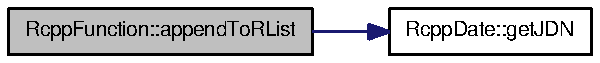
\includegraphics[width=162pt]{classRcppFunction_a9aab0b3accb81d90fb813acf3bf4c49d_cgraph}
\end{center}
\end{figure}
\hypertarget{classRcppFunction_a861ba7ae5c09acf31a034472b5a47728}{
\index{RcppFunction@{RcppFunction}!appendToRList@{appendToRList}}
\index{appendToRList@{appendToRList}!RcppFunction@{RcppFunction}}
\subsubsection[{appendToRList}]{\setlength{\rightskip}{0pt plus 5cm}void RcppFunction::appendToRList (std::string {\em name}, \/  std::string {\em value})}}
\label{classRcppFunction_a861ba7ae5c09acf31a034472b5a47728}


Definition at line 956 of file Rcpp.cpp.

References currListPosn, listArg, listSize, names, and numProtected.\hypertarget{classRcppFunction_afce449ac5d89b32e0e0b9f584278a672}{
\index{RcppFunction@{RcppFunction}!appendToRList@{appendToRList}}
\index{appendToRList@{appendToRList}!RcppFunction@{RcppFunction}}
\subsubsection[{appendToRList}]{\setlength{\rightskip}{0pt plus 5cm}void RcppFunction::appendToRList (std::string {\em name}, \/  int {\em value})}}
\label{classRcppFunction_afce449ac5d89b32e0e0b9f584278a672}


Definition at line 946 of file Rcpp.cpp.

References currListPosn, listArg, listSize, names, and numProtected.\hypertarget{classRcppFunction_a0df1a8ff093e21a2a7c6fc80d6645c7e}{
\index{RcppFunction@{RcppFunction}!appendToRList@{appendToRList}}
\index{appendToRList@{appendToRList}!RcppFunction@{RcppFunction}}
\subsubsection[{appendToRList}]{\setlength{\rightskip}{0pt plus 5cm}void RcppFunction::appendToRList (std::string {\em name}, \/  double {\em value})}}
\label{classRcppFunction_a0df1a8ff093e21a2a7c6fc80d6645c7e}


Definition at line 936 of file Rcpp.cpp.

References currListPosn, listArg, listSize, names, and numProtected.

Referenced by MyRListFunc::addOne().\hypertarget{classRcppFunction_a689c914636f0f0e86b90da4425c6e6a3}{
\index{RcppFunction@{RcppFunction}!clearProtectionStack@{clearProtectionStack}}
\index{clearProtectionStack@{clearProtectionStack}!RcppFunction@{RcppFunction}}
\subsubsection[{clearProtectionStack}]{\setlength{\rightskip}{0pt plus 5cm}void RcppFunction::clearProtectionStack ()\hspace{0.3cm}{\ttfamily  \mbox{[}inline\mbox{]}}}}
\label{classRcppFunction_a689c914636f0f0e86b90da4425c6e6a3}


Definition at line 552 of file Rcpp.h.

References numProtected.

Referenced by MyRListFunc::addOne(), and MyRVectorFunc::getSum().\hypertarget{classRcppFunction_a0cc9d29ab7db552494dddefaa78e6578}{
\index{RcppFunction@{RcppFunction}!listCall@{listCall}}
\index{listCall@{listCall}!RcppFunction@{RcppFunction}}
\subsubsection[{listCall}]{\setlength{\rightskip}{0pt plus 5cm}SEXP RcppFunction::listCall ()}}
\label{classRcppFunction_a0cc9d29ab7db552494dddefaa78e6578}


Definition at line 891 of file Rcpp.cpp.

References currListPosn, fn, listArg, listSize, names, and numProtected.

Referenced by MyRListFunc::addOne().\hypertarget{classRcppFunction_af3dbcf8dcfbdfc49ef566b5efd0ad978}{
\index{RcppFunction@{RcppFunction}!setRListSize@{setRListSize}}
\index{setRListSize@{setRListSize}!RcppFunction@{RcppFunction}}
\subsubsection[{setRListSize}]{\setlength{\rightskip}{0pt plus 5cm}void RcppFunction::setRListSize (int {\em size})}}
\label{classRcppFunction_af3dbcf8dcfbdfc49ef566b5efd0ad978}


Definition at line 930 of file Rcpp.cpp.

References listArg, listSize, and numProtected.

Referenced by MyRListFunc::addOne().\hypertarget{classRcppFunction_a482df5aa5e2a98d52c9a79cf3ab31c67}{
\index{RcppFunction@{RcppFunction}!setRVector@{setRVector}}
\index{setRVector@{setRVector}!RcppFunction@{RcppFunction}}
\subsubsection[{setRVector}]{\setlength{\rightskip}{0pt plus 5cm}void RcppFunction::setRVector (std::vector$<$ double $>$ \& {\em v})}}
\label{classRcppFunction_a482df5aa5e2a98d52c9a79cf3ab31c67}


Definition at line 923 of file Rcpp.cpp.

References numProtected, and vectorArg.

Referenced by MyRVectorFunc::getSum().\hypertarget{classRcppFunction_ac57c514c761609892ff553434e134446}{
\index{RcppFunction@{RcppFunction}!vectorCall@{vectorCall}}
\index{vectorCall@{vectorCall}!RcppFunction@{RcppFunction}}
\subsubsection[{vectorCall}]{\setlength{\rightskip}{0pt plus 5cm}SEXP RcppFunction::vectorCall ()}}
\label{classRcppFunction_ac57c514c761609892ff553434e134446}


Definition at line 911 of file Rcpp.cpp.

References fn, numProtected, and vectorArg.

Referenced by MyRVectorFunc::getSum().

\subsection{Member Data Documentation}
\hypertarget{classRcppFunction_ace513a92e96b36883b709b5352ea5663}{
\index{RcppFunction@{RcppFunction}!currListPosn@{currListPosn}}
\index{currListPosn@{currListPosn}!RcppFunction@{RcppFunction}}
\subsubsection[{currListPosn}]{\setlength{\rightskip}{0pt plus 5cm}int {\bf RcppFunction::currListPosn}\hspace{0.3cm}{\ttfamily  \mbox{[}private\mbox{]}}}}
\label{classRcppFunction_ace513a92e96b36883b709b5352ea5663}


Definition at line 559 of file Rcpp.h.

Referenced by appendToRList(), listCall(), and RcppFunction().\hypertarget{classRcppFunction_aa6b5966224b8b7d158be6cdfc3612063}{
\index{RcppFunction@{RcppFunction}!fn@{fn}}
\index{fn@{fn}!RcppFunction@{RcppFunction}}
\subsubsection[{fn}]{\setlength{\rightskip}{0pt plus 5cm}SEXP {\bf RcppFunction::fn}\hspace{0.3cm}{\ttfamily  \mbox{[}private\mbox{]}}}}
\label{classRcppFunction_aa6b5966224b8b7d158be6cdfc3612063}


Definition at line 558 of file Rcpp.h.

Referenced by listCall(), and vectorCall().\hypertarget{classRcppFunction_a3b8a2c8441c9791f9fe5bd5273bbceec}{
\index{RcppFunction@{RcppFunction}!listArg@{listArg}}
\index{listArg@{listArg}!RcppFunction@{RcppFunction}}
\subsubsection[{listArg}]{\setlength{\rightskip}{0pt plus 5cm}SEXP {\bf RcppFunction::listArg}\hspace{0.3cm}{\ttfamily  \mbox{[}private\mbox{]}}}}
\label{classRcppFunction_a3b8a2c8441c9791f9fe5bd5273bbceec}


Definition at line 558 of file Rcpp.h.

Referenced by appendToRList(), listCall(), RcppFunction(), and setRListSize().\hypertarget{classRcppFunction_ac3a42478ffd123f430ba3e09099db6f8}{
\index{RcppFunction@{RcppFunction}!listSize@{listSize}}
\index{listSize@{listSize}!RcppFunction@{RcppFunction}}
\subsubsection[{listSize}]{\setlength{\rightskip}{0pt plus 5cm}int {\bf RcppFunction::listSize}\hspace{0.3cm}{\ttfamily  \mbox{[}private\mbox{]}}}}
\label{classRcppFunction_ac3a42478ffd123f430ba3e09099db6f8}


Definition at line 559 of file Rcpp.h.

Referenced by appendToRList(), listCall(), RcppFunction(), and setRListSize().\hypertarget{classRcppFunction_abf9e86df5e1a290a5f321e6051f0d2b2}{
\index{RcppFunction@{RcppFunction}!names@{names}}
\index{names@{names}!RcppFunction@{RcppFunction}}
\subsubsection[{names}]{\setlength{\rightskip}{0pt plus 5cm}std::vector$<$std::string$>$ {\bf RcppFunction::names}\hspace{0.3cm}{\ttfamily  \mbox{[}private\mbox{]}}}}
\label{classRcppFunction_abf9e86df5e1a290a5f321e6051f0d2b2}


Definition at line 560 of file Rcpp.h.

Referenced by appendToRList(), and listCall().\hypertarget{classRcppFunction_adc777e7d1628ccc4f531a8375f30f385}{
\index{RcppFunction@{RcppFunction}!numProtected@{numProtected}}
\index{numProtected@{numProtected}!RcppFunction@{RcppFunction}}
\subsubsection[{numProtected}]{\setlength{\rightskip}{0pt plus 5cm}int {\bf RcppFunction::numProtected}\hspace{0.3cm}{\ttfamily  \mbox{[}private\mbox{]}}}}
\label{classRcppFunction_adc777e7d1628ccc4f531a8375f30f385}


Definition at line 559 of file Rcpp.h.

Referenced by appendToRList(), clearProtectionStack(), listCall(), RcppFunction(), setRListSize(), setRVector(), vectorCall(), and $\sim$RcppFunction().\hypertarget{classRcppFunction_a0492c128c0f72cda44e679265b36b50e}{
\index{RcppFunction@{RcppFunction}!vectorArg@{vectorArg}}
\index{vectorArg@{vectorArg}!RcppFunction@{RcppFunction}}
\subsubsection[{vectorArg}]{\setlength{\rightskip}{0pt plus 5cm}SEXP {\bf RcppFunction::vectorArg}\hspace{0.3cm}{\ttfamily  \mbox{[}private\mbox{]}}}}
\label{classRcppFunction_a0492c128c0f72cda44e679265b36b50e}


Definition at line 558 of file Rcpp.h.

Referenced by RcppFunction(), setRVector(), and vectorCall().

The documentation for this class was generated from the following files:\begin{DoxyCompactItemize}
\item 
src/\hyperlink{Rcpp_8h}{Rcpp.h}\item 
src/\hyperlink{Rcpp_8cpp}{Rcpp.cpp}\end{DoxyCompactItemize}

\hypertarget{classRcppMatrix}{
\section{RcppMatrix$<$ T $>$ Class Template Reference}
\label{classRcppMatrix}\index{RcppMatrix@{RcppMatrix}}
}
{\tt \#include $<$Rcpp.h$>$}

Collaboration diagram for RcppMatrix$<$ T $>$:\nopagebreak
\begin{figure}[H]
\begin{center}
\leavevmode
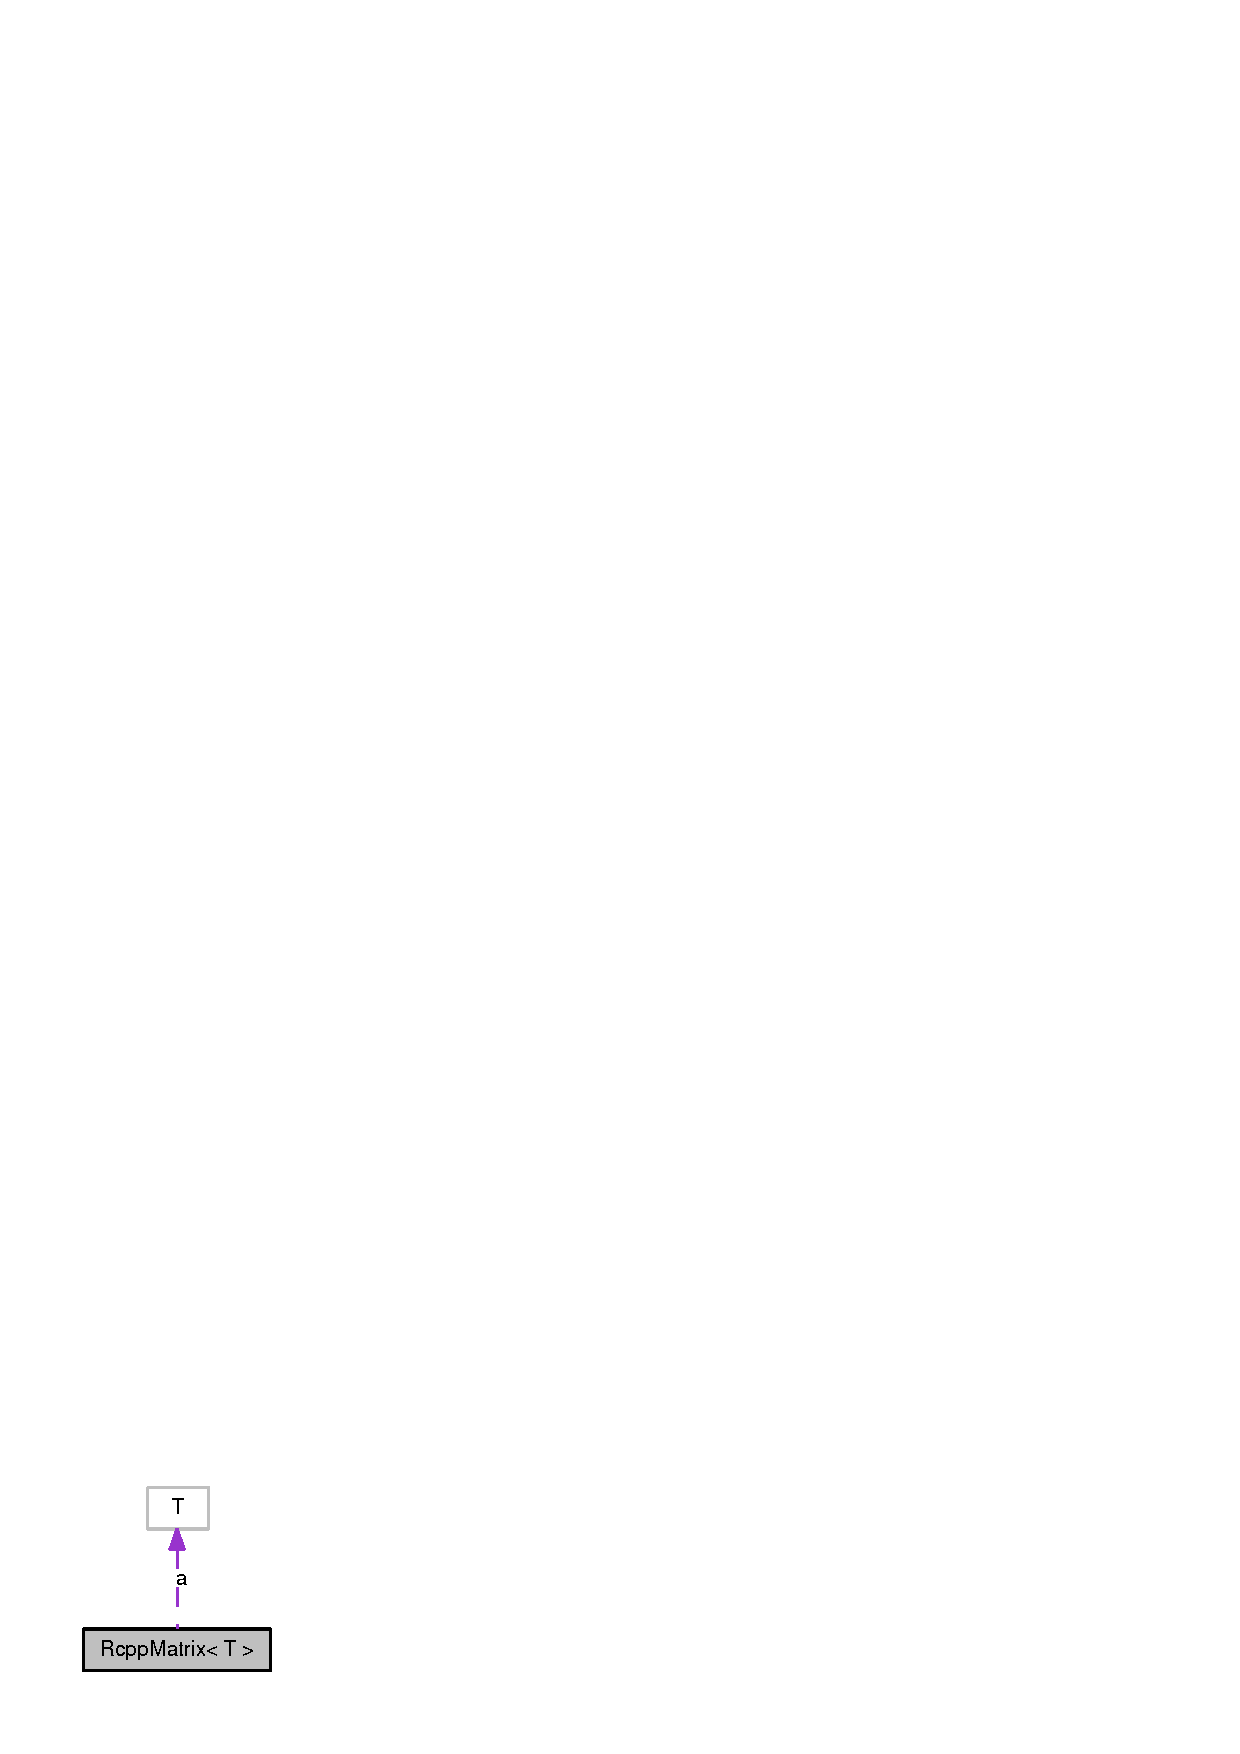
\includegraphics[width=67pt]{classRcppMatrix__coll__graph}
\end{center}
\end{figure}
\subsection*{Public Member Functions}
\begin{CompactItemize}
\item 
\hyperlink{classRcppMatrix_6cdd09180c21b504d1455ae2bc8939a7}{RcppMatrix} (SEXP mat)
\item 
\hyperlink{classRcppMatrix_9ac16e2fcccd2a21a33097139e4ec253}{RcppMatrix} (int nx, int ny)
\item 
int \hyperlink{classRcppMatrix_edbe27d643d704a0f5a995821307fdaf}{getDim1} ()
\item 
int \hyperlink{classRcppMatrix_356e04f844e3ebfac29b50e2e749734f}{getDim2} ()
\item 
T \& \hyperlink{classRcppMatrix_7733c87524d7e216f70fc10ccc971a29}{operator()} (int i, int j)
\item 
T $\ast$$\ast$ \hyperlink{classRcppMatrix_e94a95b2125bd594965e26a93c994da4}{cMatrix} ()
\item 
std::vector$<$ std::vector$<$ T $>$ $>$ \hyperlink{classRcppMatrix_e74547edb5d989adb87b2e483153de89}{stlMatrix} ()
\end{CompactItemize}
\subsection*{Private Attributes}
\begin{CompactItemize}
\item 
int \hyperlink{classRcppMatrix_3b2f3ef7c2b482e4f7e7f4f96b787128}{dim1}
\item 
int \hyperlink{classRcppMatrix_d01bc64d89dcc475f7c90f1580bf5d52}{dim2}
\item 
T $\ast$$\ast$ \hyperlink{classRcppMatrix_3f4dad8e2aed525c9b20e98d262ec31e}{a}
\end{CompactItemize}


\subsection{Detailed Description}
\subsubsection*{template$<$typename T$>$ class RcppMatrix$<$ T $>$}



Definition at line 445 of file Rcpp.h.

\subsection{Constructor \& Destructor Documentation}
\hypertarget{classRcppMatrix_6cdd09180c21b504d1455ae2bc8939a7}{
\index{RcppMatrix@{RcppMatrix}!RcppMatrix@{RcppMatrix}}
\index{RcppMatrix@{RcppMatrix}!RcppMatrix@{RcppMatrix}}
\subsubsection[RcppMatrix]{\setlength{\rightskip}{0pt plus 5cm}template$<$typename T$>$ {\bf RcppMatrix}$<$ T $>$::{\bf RcppMatrix} (SEXP {\em mat})\hspace{0.3cm}{\tt  \mbox{[}inline\mbox{]}}}}
\label{classRcppMatrix_6cdd09180c21b504d1455ae2bc8939a7}




Definition at line 338 of file Rcpp.cpp.

References RcppMatrix$<$ T $>$::a, RcppMatrix$<$ T $>$::dim1, and RcppMatrix$<$ T $>$::dim2.\hypertarget{classRcppMatrix_9ac16e2fcccd2a21a33097139e4ec253}{
\index{RcppMatrix@{RcppMatrix}!RcppMatrix@{RcppMatrix}}
\index{RcppMatrix@{RcppMatrix}!RcppMatrix@{RcppMatrix}}
\subsubsection[RcppMatrix]{\setlength{\rightskip}{0pt plus 5cm}template$<$typename T$>$ {\bf RcppMatrix}$<$ T $>$::{\bf RcppMatrix} (int {\em nx}, \/  int {\em ny})\hspace{0.3cm}{\tt  \mbox{[}inline\mbox{]}}}}
\label{classRcppMatrix_9ac16e2fcccd2a21a33097139e4ec253}




Definition at line 369 of file Rcpp.cpp.

References RcppMatrix$<$ T $>$::a, RcppMatrix$<$ T $>$::dim1, and RcppMatrix$<$ T $>$::dim2.

\subsection{Member Function Documentation}
\hypertarget{classRcppMatrix_edbe27d643d704a0f5a995821307fdaf}{
\index{RcppMatrix@{RcppMatrix}!getDim1@{getDim1}}
\index{getDim1@{getDim1}!RcppMatrix@{RcppMatrix}}
\subsubsection[getDim1]{\setlength{\rightskip}{0pt plus 5cm}template$<$typename T$>$ int {\bf RcppMatrix}$<$ T $>$::getDim1 ()\hspace{0.3cm}{\tt  \mbox{[}inline\mbox{]}}}}
\label{classRcppMatrix_edbe27d643d704a0f5a995821307fdaf}




Definition at line 449 of file Rcpp.h.

References RcppMatrix$<$ T $>$::dim1.

Referenced by RcppResultSet::add(), and Rcpp\_\-Example().\hypertarget{classRcppMatrix_356e04f844e3ebfac29b50e2e749734f}{
\index{RcppMatrix@{RcppMatrix}!getDim2@{getDim2}}
\index{getDim2@{getDim2}!RcppMatrix@{RcppMatrix}}
\subsubsection[getDim2]{\setlength{\rightskip}{0pt plus 5cm}template$<$typename T$>$ int {\bf RcppMatrix}$<$ T $>$::getDim2 ()\hspace{0.3cm}{\tt  \mbox{[}inline\mbox{]}}}}
\label{classRcppMatrix_356e04f844e3ebfac29b50e2e749734f}




Definition at line 450 of file Rcpp.h.

References RcppMatrix$<$ T $>$::dim2.

Referenced by RcppResultSet::add(), and Rcpp\_\-Example().\hypertarget{classRcppMatrix_7733c87524d7e216f70fc10ccc971a29}{
\index{RcppMatrix@{RcppMatrix}!operator()@{operator()}}
\index{operator()@{operator()}!RcppMatrix@{RcppMatrix}}
\subsubsection[operator()]{\setlength{\rightskip}{0pt plus 5cm}template$<$typename T$>$ T\& {\bf RcppMatrix}$<$ T $>$::operator() (int {\em i}, \/  int {\em j})\hspace{0.3cm}{\tt  \mbox{[}inline\mbox{]}}}}
\label{classRcppMatrix_7733c87524d7e216f70fc10ccc971a29}




Definition at line 451 of file Rcpp.h.

References RcppMatrix$<$ T $>$::a, RcppMatrix$<$ T $>$::dim1, and RcppMatrix$<$ T $>$::dim2.\hypertarget{classRcppMatrix_e94a95b2125bd594965e26a93c994da4}{
\index{RcppMatrix@{RcppMatrix}!cMatrix@{cMatrix}}
\index{cMatrix@{cMatrix}!RcppMatrix@{RcppMatrix}}
\subsubsection[cMatrix]{\setlength{\rightskip}{0pt plus 5cm}template$<$typename T$>$ T $\ast$$\ast$ {\bf RcppMatrix}$<$ T $>$::cMatrix ()\hspace{0.3cm}{\tt  \mbox{[}inline\mbox{]}}}}
\label{classRcppMatrix_e94a95b2125bd594965e26a93c994da4}




Definition at line 396 of file Rcpp.cpp.

References RcppMatrix$<$ T $>$::a, RcppMatrix$<$ T $>$::dim1, and RcppMatrix$<$ T $>$::dim2.

Referenced by RcppResultSet::add(), and Rcpp\_\-Example().\hypertarget{classRcppMatrix_e74547edb5d989adb87b2e483153de89}{
\index{RcppMatrix@{RcppMatrix}!stlMatrix@{stlMatrix}}
\index{stlMatrix@{stlMatrix}!RcppMatrix@{RcppMatrix}}
\subsubsection[stlMatrix]{\setlength{\rightskip}{0pt plus 5cm}template$<$typename T$>$ std::vector$<$ std::vector$<$ T $>$ $>$ {\bf RcppMatrix}$<$ T $>$::stlMatrix ()\hspace{0.3cm}{\tt  \mbox{[}inline\mbox{]}}}}
\label{classRcppMatrix_e74547edb5d989adb87b2e483153de89}




Definition at line 383 of file Rcpp.cpp.

References RcppMatrix$<$ T $>$::a, RcppMatrix$<$ T $>$::dim1, and RcppMatrix$<$ T $>$::dim2.

Referenced by Rcpp\_\-Example().

\subsection{Member Data Documentation}
\hypertarget{classRcppMatrix_3b2f3ef7c2b482e4f7e7f4f96b787128}{
\index{RcppMatrix@{RcppMatrix}!dim1@{dim1}}
\index{dim1@{dim1}!RcppMatrix@{RcppMatrix}}
\subsubsection[dim1]{\setlength{\rightskip}{0pt plus 5cm}template$<$typename T$>$ int {\bf RcppMatrix}$<$ T $>$::{\bf dim1}\hspace{0.3cm}{\tt  \mbox{[}private\mbox{]}}}}
\label{classRcppMatrix_3b2f3ef7c2b482e4f7e7f4f96b787128}




Definition at line 462 of file Rcpp.h.

Referenced by RcppMatrix$<$ T $>$::cMatrix(), RcppMatrix$<$ T $>$::getDim1(), RcppMatrix$<$ T $>$::operator()(), RcppMatrix$<$ T $>$::RcppMatrix(), and RcppMatrix$<$ T $>$::stlMatrix().\hypertarget{classRcppMatrix_d01bc64d89dcc475f7c90f1580bf5d52}{
\index{RcppMatrix@{RcppMatrix}!dim2@{dim2}}
\index{dim2@{dim2}!RcppMatrix@{RcppMatrix}}
\subsubsection[dim2]{\setlength{\rightskip}{0pt plus 5cm}template$<$typename T$>$ int {\bf RcppMatrix}$<$ T $>$::{\bf dim2}\hspace{0.3cm}{\tt  \mbox{[}private\mbox{]}}}}
\label{classRcppMatrix_d01bc64d89dcc475f7c90f1580bf5d52}




Definition at line 462 of file Rcpp.h.

Referenced by RcppMatrix$<$ T $>$::cMatrix(), RcppMatrix$<$ T $>$::getDim2(), RcppMatrix$<$ T $>$::operator()(), RcppMatrix$<$ T $>$::RcppMatrix(), and RcppMatrix$<$ T $>$::stlMatrix().\hypertarget{classRcppMatrix_3f4dad8e2aed525c9b20e98d262ec31e}{
\index{RcppMatrix@{RcppMatrix}!a@{a}}
\index{a@{a}!RcppMatrix@{RcppMatrix}}
\subsubsection[a]{\setlength{\rightskip}{0pt plus 5cm}template$<$typename T$>$ T$\ast$$\ast$ {\bf RcppMatrix}$<$ T $>$::{\bf a}\hspace{0.3cm}{\tt  \mbox{[}private\mbox{]}}}}
\label{classRcppMatrix_3f4dad8e2aed525c9b20e98d262ec31e}




Definition at line 463 of file Rcpp.h.

Referenced by RcppMatrix$<$ T $>$::cMatrix(), RcppMatrix$<$ T $>$::operator()(), RcppMatrix$<$ T $>$::RcppMatrix(), and RcppMatrix$<$ T $>$::stlMatrix().

The documentation for this class was generated from the following files:\begin{CompactItemize}
\item 
src/\hyperlink{Rcpp_8h}{Rcpp.h}\item 
src/\hyperlink{Rcpp_8cpp}{Rcpp.cpp}\end{CompactItemize}

\hypertarget{classRcppMatrixView}{
\section{RcppMatrixView$<$ T $>$ Class Template Reference}
\label{classRcppMatrixView}\index{RcppMatrixView@{RcppMatrixView}}
}


{\ttfamily \#include $<$Rcpp.h$>$}\subsection*{Public Member Functions}
\begin{DoxyCompactItemize}
\item 
\hyperlink{classRcppMatrixView_ac3489c6a24c2975f3ea7103ada50e328}{RcppMatrixView} (SEXP mat)
\item 
int \hyperlink{classRcppMatrixView_a72d1d7fcdc4b1cc6dd877b1df2f9f5e6}{dim1} () const 
\item 
int \hyperlink{classRcppMatrixView_aebb7f65646ce780c897dc39f31899439}{dim2} () const 
\item 
int \hyperlink{classRcppMatrixView_a0892184e9fc01863f79d76b3751ddbdb}{rows} ()
\item 
int \hyperlink{classRcppMatrixView_a037e6fee7e029eef53c35a63f11e2e2a}{cols} ()
\item 
T \hyperlink{classRcppMatrixView_ad135a7e855eee55b078807766aff9e96}{operator()} (int i, int j) const 
\end{DoxyCompactItemize}
\subsection*{Private Attributes}
\begin{DoxyCompactItemize}
\item 
int \hyperlink{classRcppMatrixView_ad492401691ef709f6d2ef7dc1dcc2134}{d1}
\item 
int \hyperlink{classRcppMatrixView_a37b5f5806957eeb0b688d6a157a2a264}{d2}
\item 
T $\ast$ \hyperlink{classRcppMatrixView_ad38481118f63a84a132e8f2265de5bdd}{a}
\end{DoxyCompactItemize}


\subsection{Detailed Description}
\subsubsection*{template$<$typename T$>$ class RcppMatrixView$<$ T $>$}



Definition at line 492 of file Rcpp.h.

\subsection{Constructor \& Destructor Documentation}
\hypertarget{classRcppMatrixView_ac3489c6a24c2975f3ea7103ada50e328}{
\index{RcppMatrixView@{RcppMatrixView}!RcppMatrixView@{RcppMatrixView}}
\index{RcppMatrixView@{RcppMatrixView}!RcppMatrixView@{RcppMatrixView}}
\subsubsection[{RcppMatrixView}]{\setlength{\rightskip}{0pt plus 5cm}template$<$typename T $>$ {\bf RcppMatrixView}$<$ T $>$::{\bf RcppMatrixView} (SEXP {\em mat})\hspace{0.3cm}{\ttfamily  \mbox{[}inline\mbox{]}}}}
\label{classRcppMatrixView_ac3489c6a24c2975f3ea7103ada50e328}


Definition at line 436 of file Rcpp.cpp.

References RcppMatrixView$<$ T $>$::a, RcppMatrixView$<$ T $>$::d1, and RcppMatrixView$<$ T $>$::d2.

\subsection{Member Function Documentation}
\hypertarget{classRcppMatrixView_a037e6fee7e029eef53c35a63f11e2e2a}{
\index{RcppMatrixView@{RcppMatrixView}!cols@{cols}}
\index{cols@{cols}!RcppMatrixView@{RcppMatrixView}}
\subsubsection[{cols}]{\setlength{\rightskip}{0pt plus 5cm}template$<$typename T $>$ int {\bf RcppMatrixView}$<$ T $>$::cols ()\hspace{0.3cm}{\ttfamily  \mbox{[}inline\mbox{]}}}}
\label{classRcppMatrixView_a037e6fee7e029eef53c35a63f11e2e2a}


Definition at line 498 of file Rcpp.h.

References RcppMatrixView$<$ T $>$::d2.\hypertarget{classRcppMatrixView_a72d1d7fcdc4b1cc6dd877b1df2f9f5e6}{
\index{RcppMatrixView@{RcppMatrixView}!dim1@{dim1}}
\index{dim1@{dim1}!RcppMatrixView@{RcppMatrixView}}
\subsubsection[{dim1}]{\setlength{\rightskip}{0pt plus 5cm}template$<$typename T $>$ int {\bf RcppMatrixView}$<$ T $>$::dim1 () const\hspace{0.3cm}{\ttfamily  \mbox{[}inline\mbox{]}}}}
\label{classRcppMatrixView_a72d1d7fcdc4b1cc6dd877b1df2f9f5e6}


Definition at line 495 of file Rcpp.h.

References RcppMatrixView$<$ T $>$::d1.\hypertarget{classRcppMatrixView_aebb7f65646ce780c897dc39f31899439}{
\index{RcppMatrixView@{RcppMatrixView}!dim2@{dim2}}
\index{dim2@{dim2}!RcppMatrixView@{RcppMatrixView}}
\subsubsection[{dim2}]{\setlength{\rightskip}{0pt plus 5cm}template$<$typename T $>$ int {\bf RcppMatrixView}$<$ T $>$::dim2 () const\hspace{0.3cm}{\ttfamily  \mbox{[}inline\mbox{]}}}}
\label{classRcppMatrixView_aebb7f65646ce780c897dc39f31899439}


Definition at line 496 of file Rcpp.h.

References RcppMatrixView$<$ T $>$::d2.\hypertarget{classRcppMatrixView_ad135a7e855eee55b078807766aff9e96}{
\index{RcppMatrixView@{RcppMatrixView}!operator()@{operator()}}
\index{operator()@{operator()}!RcppMatrixView@{RcppMatrixView}}
\subsubsection[{operator()}]{\setlength{\rightskip}{0pt plus 5cm}template$<$typename T $>$ T {\bf RcppMatrixView}$<$ T $>$::operator() (int {\em i}, \/  int {\em j}) const\hspace{0.3cm}{\ttfamily  \mbox{[}inline\mbox{]}}}}
\label{classRcppMatrixView_ad135a7e855eee55b078807766aff9e96}


Definition at line 499 of file Rcpp.h.

References RcppMatrixView$<$ T $>$::a, RcppMatrixView$<$ T $>$::d1, and RcppMatrixView$<$ T $>$::d2.\hypertarget{classRcppMatrixView_a0892184e9fc01863f79d76b3751ddbdb}{
\index{RcppMatrixView@{RcppMatrixView}!rows@{rows}}
\index{rows@{rows}!RcppMatrixView@{RcppMatrixView}}
\subsubsection[{rows}]{\setlength{\rightskip}{0pt plus 5cm}template$<$typename T $>$ int {\bf RcppMatrixView}$<$ T $>$::rows ()\hspace{0.3cm}{\ttfamily  \mbox{[}inline\mbox{]}}}}
\label{classRcppMatrixView_a0892184e9fc01863f79d76b3751ddbdb}


Definition at line 497 of file Rcpp.h.

References RcppMatrixView$<$ T $>$::d1.

\subsection{Member Data Documentation}
\hypertarget{classRcppMatrixView_ad38481118f63a84a132e8f2265de5bdd}{
\index{RcppMatrixView@{RcppMatrixView}!a@{a}}
\index{a@{a}!RcppMatrixView@{RcppMatrixView}}
\subsubsection[{a}]{\setlength{\rightskip}{0pt plus 5cm}template$<$typename T $>$ T$\ast$ {\bf RcppMatrixView}$<$ T $>$::{\bf a}\hspace{0.3cm}{\ttfamily  \mbox{[}private\mbox{]}}}}
\label{classRcppMatrixView_ad38481118f63a84a132e8f2265de5bdd}


Definition at line 509 of file Rcpp.h.

Referenced by RcppMatrixView$<$ T $>$::operator()(), and RcppMatrixView$<$ T $>$::RcppMatrixView().\hypertarget{classRcppMatrixView_ad492401691ef709f6d2ef7dc1dcc2134}{
\index{RcppMatrixView@{RcppMatrixView}!d1@{d1}}
\index{d1@{d1}!RcppMatrixView@{RcppMatrixView}}
\subsubsection[{d1}]{\setlength{\rightskip}{0pt plus 5cm}template$<$typename T $>$ int {\bf RcppMatrixView}$<$ T $>$::{\bf d1}\hspace{0.3cm}{\ttfamily  \mbox{[}private\mbox{]}}}}
\label{classRcppMatrixView_ad492401691ef709f6d2ef7dc1dcc2134}


Definition at line 508 of file Rcpp.h.

Referenced by RcppMatrixView$<$ T $>$::dim1(), RcppMatrixView$<$ T $>$::operator()(), RcppMatrixView$<$ T $>$::RcppMatrixView(), and RcppMatrixView$<$ T $>$::rows().\hypertarget{classRcppMatrixView_a37b5f5806957eeb0b688d6a157a2a264}{
\index{RcppMatrixView@{RcppMatrixView}!d2@{d2}}
\index{d2@{d2}!RcppMatrixView@{RcppMatrixView}}
\subsubsection[{d2}]{\setlength{\rightskip}{0pt plus 5cm}template$<$typename T $>$ int {\bf RcppMatrixView}$<$ T $>$::{\bf d2}\hspace{0.3cm}{\ttfamily  \mbox{[}private\mbox{]}}}}
\label{classRcppMatrixView_a37b5f5806957eeb0b688d6a157a2a264}


Definition at line 508 of file Rcpp.h.

Referenced by RcppMatrixView$<$ T $>$::cols(), RcppMatrixView$<$ T $>$::dim2(), RcppMatrixView$<$ T $>$::operator()(), and RcppMatrixView$<$ T $>$::RcppMatrixView().

The documentation for this class was generated from the following files:\begin{DoxyCompactItemize}
\item 
src/\hyperlink{Rcpp_8h}{Rcpp.h}\item 
src/\hyperlink{Rcpp_8cpp}{Rcpp.cpp}\end{DoxyCompactItemize}

\hypertarget{classRcppNumList}{
\section{RcppNumList Class Reference}
\label{classRcppNumList}\index{RcppNumList@{RcppNumList}}
}
{\tt \#include $<$Rcpp.h$>$}

\subsection*{Public Member Functions}
\begin{CompactItemize}
\item 
\hyperlink{classRcppNumList_4a8a321d0dc84b6d4be988005fa74fcd}{RcppNumList} (SEXP theList)
\item 
std::string \hyperlink{classRcppNumList_246d8e534d97fbe798b8567bbfa93ca7}{getName} (int i)
\item 
double \hyperlink{classRcppNumList_2e83950933ddc73ad64ed800f6f5e23b}{getValue} (int i)
\item 
int \hyperlink{classRcppNumList_18dc0660cc827bcf17d9738cb5874db7}{size} ()
\end{CompactItemize}
\subsection*{Private Attributes}
\begin{CompactItemize}
\item 
int \hyperlink{classRcppNumList_c4cb5c784f7105f0f28ae48d02deb3a1}{len}
\item 
SEXP \hyperlink{classRcppNumList_7464927aafe555a0c4a104247dba7185}{namedList}
\item 
SEXP \hyperlink{classRcppNumList_a669b28cba0c95531a3c92910a60ecb0}{names}
\end{CompactItemize}


\subsection{Detailed Description}


Definition at line 319 of file Rcpp.h.

\subsection{Constructor \& Destructor Documentation}
\hypertarget{classRcppNumList_4a8a321d0dc84b6d4be988005fa74fcd}{
\index{RcppNumList@{RcppNumList}!RcppNumList@{RcppNumList}}
\index{RcppNumList@{RcppNumList}!RcppNumList@{RcppNumList}}
\subsubsection[{RcppNumList}]{\setlength{\rightskip}{0pt plus 5cm}RcppNumList::RcppNumList (SEXP {\em theList})\hspace{0.3cm}{\tt  \mbox{[}inline\mbox{]}}}}
\label{classRcppNumList_4a8a321d0dc84b6d4be988005fa74fcd}




Definition at line 321 of file Rcpp.h.

References len, namedList, and names.

\subsection{Member Function Documentation}
\hypertarget{classRcppNumList_246d8e534d97fbe798b8567bbfa93ca7}{
\index{RcppNumList@{RcppNumList}!getName@{getName}}
\index{getName@{getName}!RcppNumList@{RcppNumList}}
\subsubsection[{getName}]{\setlength{\rightskip}{0pt plus 5cm}std::string RcppNumList::getName (int {\em i})\hspace{0.3cm}{\tt  \mbox{[}inline\mbox{]}}}}
\label{classRcppNumList_246d8e534d97fbe798b8567bbfa93ca7}




Definition at line 328 of file Rcpp.h.

References len, and names.

Referenced by Rcpp\_\-Example().\hypertarget{classRcppNumList_2e83950933ddc73ad64ed800f6f5e23b}{
\index{RcppNumList@{RcppNumList}!getValue@{getValue}}
\index{getValue@{getValue}!RcppNumList@{RcppNumList}}
\subsubsection[{getValue}]{\setlength{\rightskip}{0pt plus 5cm}double RcppNumList::getValue (int {\em i})\hspace{0.3cm}{\tt  \mbox{[}inline\mbox{]}}}}
\label{classRcppNumList_2e83950933ddc73ad64ed800f6f5e23b}




Definition at line 336 of file Rcpp.h.

References len, and namedList.

Referenced by Rcpp\_\-Example().\hypertarget{classRcppNumList_18dc0660cc827bcf17d9738cb5874db7}{
\index{RcppNumList@{RcppNumList}!size@{size}}
\index{size@{size}!RcppNumList@{RcppNumList}}
\subsubsection[{size}]{\setlength{\rightskip}{0pt plus 5cm}int RcppNumList::size ()\hspace{0.3cm}{\tt  \mbox{[}inline\mbox{]}}}}
\label{classRcppNumList_18dc0660cc827bcf17d9738cb5874db7}




Definition at line 351 of file Rcpp.h.

References len.

\subsection{Member Data Documentation}
\hypertarget{classRcppNumList_c4cb5c784f7105f0f28ae48d02deb3a1}{
\index{RcppNumList@{RcppNumList}!len@{len}}
\index{len@{len}!RcppNumList@{RcppNumList}}
\subsubsection[{len}]{\setlength{\rightskip}{0pt plus 5cm}int {\bf RcppNumList::len}\hspace{0.3cm}{\tt  \mbox{[}private\mbox{]}}}}
\label{classRcppNumList_c4cb5c784f7105f0f28ae48d02deb3a1}




Definition at line 353 of file Rcpp.h.

Referenced by getName(), getValue(), RcppNumList(), and size().\hypertarget{classRcppNumList_7464927aafe555a0c4a104247dba7185}{
\index{RcppNumList@{RcppNumList}!namedList@{namedList}}
\index{namedList@{namedList}!RcppNumList@{RcppNumList}}
\subsubsection[{namedList}]{\setlength{\rightskip}{0pt plus 5cm}SEXP {\bf RcppNumList::namedList}\hspace{0.3cm}{\tt  \mbox{[}private\mbox{]}}}}
\label{classRcppNumList_7464927aafe555a0c4a104247dba7185}




Definition at line 354 of file Rcpp.h.

Referenced by getValue(), and RcppNumList().\hypertarget{classRcppNumList_a669b28cba0c95531a3c92910a60ecb0}{
\index{RcppNumList@{RcppNumList}!names@{names}}
\index{names@{names}!RcppNumList@{RcppNumList}}
\subsubsection[{names}]{\setlength{\rightskip}{0pt plus 5cm}SEXP {\bf RcppNumList::names}\hspace{0.3cm}{\tt  \mbox{[}private\mbox{]}}}}
\label{classRcppNumList_a669b28cba0c95531a3c92910a60ecb0}




Definition at line 355 of file Rcpp.h.

Referenced by getName(), and RcppNumList().

The documentation for this class was generated from the following file:\begin{CompactItemize}
\item 
src/\hyperlink{Rcpp_8h}{Rcpp.h}\end{CompactItemize}

\hypertarget{classRcppParams}{
\section{RcppParams Class Reference}
\label{classRcppParams}\index{RcppParams@{RcppParams}}
}


{\ttfamily \#include $<$Rcpp.h$>$}\subsection*{Public Member Functions}
\begin{DoxyCompactItemize}
\item 
\hyperlink{classRcppParams_a7315d083ee0d1d0ca00c3aad0175d524}{RcppParams} (SEXP params)
\item 
void \hyperlink{classRcppParams_a1b8feaf39d3ffdf0f6773c44ac53736c}{checkNames} (char $\ast$inputNames\mbox{[}$\,$\mbox{]}, int len)
\item 
bool \hyperlink{classRcppParams_a989141ab2a8800b97d91bfb43420c6bc}{exists} (std::string name)
\item 
double \hyperlink{classRcppParams_aa45f8bc1cd8a64aa9a98e24158407077}{getDoubleValue} (std::string name)
\item 
int \hyperlink{classRcppParams_abb554151641ab12a793f28d3d081973a}{getIntValue} (std::string name)
\item 
std::string \hyperlink{classRcppParams_adc04f4552582eeec09b0806ddd8e2581}{getStringValue} (std::string name)
\item 
bool \hyperlink{classRcppParams_ad818a50a0e269360f3f74c5259dec882}{getBoolValue} (std::string name)
\item 
\hyperlink{classRcppDate}{RcppDate} \hyperlink{classRcppParams_aae20c7ee73aa2f1176837cc9387ad008}{getDateValue} (std::string name)
\item 
\hyperlink{classRcppDatetime}{RcppDatetime} \hyperlink{classRcppParams_aa4bec8bfe32d5079e64dc1c9a8fcf1b9}{getDatetimeValue} (std::string name)
\end{DoxyCompactItemize}
\subsection*{Private Attributes}
\begin{DoxyCompactItemize}
\item 
std::map$<$ std::string, int $>$ \hyperlink{classRcppParams_a399697fc90ba3136c61dd6e20931bd8b}{pmap}
\item 
SEXP \hyperlink{classRcppParams_a3040dda3b32eff66fb73d3ba3874ca5b}{\_\-params}
\end{DoxyCompactItemize}


\subsection{Detailed Description}


Definition at line 151 of file Rcpp.h.

\subsection{Constructor \& Destructor Documentation}
\hypertarget{classRcppParams_a7315d083ee0d1d0ca00c3aad0175d524}{
\index{RcppParams@{RcppParams}!RcppParams@{RcppParams}}
\index{RcppParams@{RcppParams}!RcppParams@{RcppParams}}
\subsubsection[{RcppParams}]{\setlength{\rightskip}{0pt plus 5cm}RcppParams::RcppParams (SEXP {\em params})}}
\label{classRcppParams_a7315d083ee0d1d0ca00c3aad0175d524}


Definition at line 24 of file Rcpp.cpp.

References \_\-params, and pmap.

\subsection{Member Function Documentation}
\hypertarget{classRcppParams_a1b8feaf39d3ffdf0f6773c44ac53736c}{
\index{RcppParams@{RcppParams}!checkNames@{checkNames}}
\index{checkNames@{checkNames}!RcppParams@{RcppParams}}
\subsubsection[{checkNames}]{\setlength{\rightskip}{0pt plus 5cm}void RcppParams::checkNames (char $\ast$ {\em inputNames}\mbox{[}$\,$\mbox{]}, \/  int {\em len})}}
\label{classRcppParams_a1b8feaf39d3ffdf0f6773c44ac53736c}


Definition at line 40 of file Rcpp.cpp.

References pmap.\hypertarget{classRcppParams_a989141ab2a8800b97d91bfb43420c6bc}{
\index{RcppParams@{RcppParams}!exists@{exists}}
\index{exists@{exists}!RcppParams@{RcppParams}}
\subsubsection[{exists}]{\setlength{\rightskip}{0pt plus 5cm}bool RcppParams::exists (std::string {\em name})}}
\label{classRcppParams_a989141ab2a8800b97d91bfb43420c6bc}


Definition at line 50 of file Rcpp.cpp.

References pmap.\hypertarget{classRcppParams_ad818a50a0e269360f3f74c5259dec882}{
\index{RcppParams@{RcppParams}!getBoolValue@{getBoolValue}}
\index{getBoolValue@{getBoolValue}!RcppParams@{RcppParams}}
\subsubsection[{getBoolValue}]{\setlength{\rightskip}{0pt plus 5cm}bool RcppParams::getBoolValue (std::string {\em name})}}
\label{classRcppParams_ad818a50a0e269360f3f74c5259dec882}


Definition at line 178 of file Rcpp.cpp.

References \_\-params, and pmap.\hypertarget{classRcppParams_aa4bec8bfe32d5079e64dc1c9a8fcf1b9}{
\index{RcppParams@{RcppParams}!getDatetimeValue@{getDatetimeValue}}
\index{getDatetimeValue@{getDatetimeValue}!RcppParams@{RcppParams}}
\subsubsection[{getDatetimeValue}]{\setlength{\rightskip}{0pt plus 5cm}{\bf RcppDatetime} RcppParams::getDatetimeValue (std::string {\em name})}}
\label{classRcppParams_aa4bec8bfe32d5079e64dc1c9a8fcf1b9}


Definition at line 235 of file Rcpp.cpp.

References \_\-params, and pmap.\hypertarget{classRcppParams_aae20c7ee73aa2f1176837cc9387ad008}{
\index{RcppParams@{RcppParams}!getDateValue@{getDateValue}}
\index{getDateValue@{getDateValue}!RcppParams@{RcppParams}}
\subsubsection[{getDateValue}]{\setlength{\rightskip}{0pt plus 5cm}{\bf RcppDate} RcppParams::getDateValue (std::string {\em name})}}
\label{classRcppParams_aae20c7ee73aa2f1176837cc9387ad008}


Definition at line 212 of file Rcpp.cpp.

References \_\-params, and pmap.

Referenced by Rcpp\_\-Example(), and RcppParamsExample().\hypertarget{classRcppParams_aa45f8bc1cd8a64aa9a98e24158407077}{
\index{RcppParams@{RcppParams}!getDoubleValue@{getDoubleValue}}
\index{getDoubleValue@{getDoubleValue}!RcppParams@{RcppParams}}
\subsubsection[{getDoubleValue}]{\setlength{\rightskip}{0pt plus 5cm}double RcppParams::getDoubleValue (std::string {\em name})}}
\label{classRcppParams_aa45f8bc1cd8a64aa9a98e24158407077}


Definition at line 132 of file Rcpp.cpp.

References \_\-params, and pmap.

Referenced by Rcpp\_\-Example(), and RcppParamsExample().\hypertarget{classRcppParams_abb554151641ab12a793f28d3d081973a}{
\index{RcppParams@{RcppParams}!getIntValue@{getIntValue}}
\index{getIntValue@{getIntValue}!RcppParams@{RcppParams}}
\subsubsection[{getIntValue}]{\setlength{\rightskip}{0pt plus 5cm}int RcppParams::getIntValue (std::string {\em name})}}
\label{classRcppParams_abb554151641ab12a793f28d3d081973a}


Definition at line 155 of file Rcpp.cpp.

References \_\-params, and pmap.

Referenced by Rcpp\_\-Example(), and RcppParamsExample().\hypertarget{classRcppParams_adc04f4552582eeec09b0806ddd8e2581}{
\index{RcppParams@{RcppParams}!getStringValue@{getStringValue}}
\index{getStringValue@{getStringValue}!RcppParams@{RcppParams}}
\subsubsection[{getStringValue}]{\setlength{\rightskip}{0pt plus 5cm}std::string RcppParams::getStringValue (std::string {\em name})}}
\label{classRcppParams_adc04f4552582eeec09b0806ddd8e2581}


Definition at line 195 of file Rcpp.cpp.

References \_\-params, and pmap.

Referenced by Rcpp\_\-Example(), and RcppParamsExample().

\subsection{Member Data Documentation}
\hypertarget{classRcppParams_a3040dda3b32eff66fb73d3ba3874ca5b}{
\index{RcppParams@{RcppParams}!\_\-params@{\_\-params}}
\index{\_\-params@{\_\-params}!RcppParams@{RcppParams}}
\subsubsection[{\_\-params}]{\setlength{\rightskip}{0pt plus 5cm}SEXP {\bf RcppParams::\_\-params}\hspace{0.3cm}{\ttfamily  \mbox{[}private\mbox{]}}}}
\label{classRcppParams_a3040dda3b32eff66fb73d3ba3874ca5b}


Definition at line 164 of file Rcpp.h.

Referenced by getBoolValue(), getDatetimeValue(), getDateValue(), getDoubleValue(), getIntValue(), getStringValue(), and RcppParams().\hypertarget{classRcppParams_a399697fc90ba3136c61dd6e20931bd8b}{
\index{RcppParams@{RcppParams}!pmap@{pmap}}
\index{pmap@{pmap}!RcppParams@{RcppParams}}
\subsubsection[{pmap}]{\setlength{\rightskip}{0pt plus 5cm}std::map$<$std::string, int$>$ {\bf RcppParams::pmap}\hspace{0.3cm}{\ttfamily  \mbox{[}private\mbox{]}}}}
\label{classRcppParams_a399697fc90ba3136c61dd6e20931bd8b}


Definition at line 163 of file Rcpp.h.

Referenced by checkNames(), exists(), getBoolValue(), getDatetimeValue(), getDateValue(), getDoubleValue(), getIntValue(), getStringValue(), and RcppParams().

The documentation for this class was generated from the following files:\begin{DoxyCompactItemize}
\item 
src/\hyperlink{Rcpp_8h}{Rcpp.h}\item 
src/\hyperlink{Rcpp_8cpp}{Rcpp.cpp}\end{DoxyCompactItemize}

\hypertarget{classRcppResultSet}{
\section{RcppResultSet Class Reference}
\label{classRcppResultSet}\index{RcppResultSet@{RcppResultSet}}
}
{\tt \#include $<$Rcpp.h$>$}

\subsection*{Public Member Functions}
\begin{CompactItemize}
\item 
\hyperlink{classRcppResultSet_b799c6b9bd730e55d92228203903ba74}{RcppResultSet} ()
\item 
void \hyperlink{classRcppResultSet_7c7da37f18bd352303bf06b7c5233bc4}{add} (std::string, double)
\item 
void \hyperlink{classRcppResultSet_8b7841ff8a52477b0c6a1fb7c03c0fd9}{add} (std::string, int)
\item 
void \hyperlink{classRcppResultSet_2633372ab2f50b269e9e26dd7a489492}{add} (std::string, std::string)
\item 
void \hyperlink{classRcppResultSet_5d06d8a4f0497abc6fad4ea22b4934f9}{add} (std::string, double $\ast$, int)
\item 
void \hyperlink{classRcppResultSet_494dbe1f6db48bf48e9e33a32d897f29}{add} (std::string, int $\ast$, int)
\item 
void \hyperlink{classRcppResultSet_88ff0e3db486eec0012eb58beee05e9b}{add} (std::string, double $\ast$$\ast$, int, int)
\item 
void \hyperlink{classRcppResultSet_2cca9ea4e9554c4fad9bc326355c354c}{add} (std::string, int $\ast$$\ast$, int, int)
\item 
void \hyperlink{classRcppResultSet_e5cb861a0d6e95cc7ed465ccae2ac4a7}{add} (std::string, \hyperlink{classRcppDate}{RcppDate} \&)
\item 
void \hyperlink{classRcppResultSet_d7efd746596959ce68ca98c690a2f645}{add} (std::string, \hyperlink{classRcppDateVector}{RcppDateVector} \&)
\item 
void \hyperlink{classRcppResultSet_1d921e7a24e50369ae67a1bc63826131}{add} (std::string, \hyperlink{classRcppDatetime}{RcppDatetime} \&)
\item 
void \hyperlink{classRcppResultSet_ac8cade970247a377e8dbebf1c79a86c}{add} (std::string, \hyperlink{classRcppDatetimeVector}{RcppDatetimeVector} \&)
\item 
void \hyperlink{classRcppResultSet_10d01a24ef006c1ff14ca7e95fb9e0ea}{add} (std::string, \hyperlink{classRcppStringVector}{RcppStringVector} \&)
\item 
void \hyperlink{classRcppResultSet_2b4575ca5ccc390bc5437b1be4718ca6}{add} (std::string, std::vector$<$ double $>$ \&)
\item 
void \hyperlink{classRcppResultSet_23fa5be81281adcf3014749094816522}{add} (std::string, std::vector$<$ int $>$ \&)
\item 
void \hyperlink{classRcppResultSet_b10cd8503c12708e27068b92a83e4047}{add} (std::string, std::vector$<$ std::vector$<$ double $>$ $>$ \&)
\item 
void \hyperlink{classRcppResultSet_b51f30f4bd5f3c6153221a3bd7bb7e24}{add} (std::string, std::vector$<$ std::vector$<$ int $>$ $>$ \&)
\item 
void \hyperlink{classRcppResultSet_db4236a049c8dceb7112229f5e68a295}{add} (std::string, std::vector$<$ std::string $>$ \&)
\item 
void \hyperlink{classRcppResultSet_068cb13e27c0e26dd05e92d67eaeb7d0}{add} (std::string, \hyperlink{classRcppVector}{RcppVector}$<$ int $>$ \&)
\item 
void \hyperlink{classRcppResultSet_10a64eb042cd3bac5b635670ae2fff5d}{add} (std::string, \hyperlink{classRcppVector}{RcppVector}$<$ double $>$ \&)
\item 
void \hyperlink{classRcppResultSet_56f1bff720a6cf6503ab942bdb6892b3}{add} (std::string, \hyperlink{classRcppMatrix}{RcppMatrix}$<$ int $>$ \&)
\item 
void \hyperlink{classRcppResultSet_f6f50ca0a589fc12ef68c0406e83243b}{add} (std::string, \hyperlink{classRcppMatrix}{RcppMatrix}$<$ double $>$ \&)
\item 
void \hyperlink{classRcppResultSet_9e05fb2ca92258529ffbb536e23a2a4d}{add} (std::string, \hyperlink{classRcppFrame}{RcppFrame} \&)
\item 
void \hyperlink{classRcppResultSet_5f44a63a2cab43db551c0e27d6fec378}{add} (std::string, SEXP, bool isProtected)
\item 
SEXP \hyperlink{classRcppResultSet_916989ff6c0ed1149a5f93fb6a532946}{getReturnList} ()
\end{CompactItemize}
\subsection*{Protected Attributes}
\begin{CompactItemize}
\item 
int \hyperlink{classRcppResultSet_19edd02ac05783f9b4fd840c22e74153}{numProtected}
\item 
std::list$<$ std::pair$<$ std::string, SEXP $>$ $>$ \hyperlink{classRcppResultSet_509f3d779c88476dea89ade9c08d403f}{values}
\end{CompactItemize}


\subsection{Detailed Description}


Definition at line 558 of file Rcpp.h.

\subsection{Constructor \& Destructor Documentation}
\hypertarget{classRcppResultSet_b799c6b9bd730e55d92228203903ba74}{
\index{RcppResultSet@{RcppResultSet}!RcppResultSet@{RcppResultSet}}
\index{RcppResultSet@{RcppResultSet}!RcppResultSet@{RcppResultSet}}
\subsubsection[{RcppResultSet}]{\setlength{\rightskip}{0pt plus 5cm}RcppResultSet::RcppResultSet ()\hspace{0.3cm}{\tt  \mbox{[}inline\mbox{]}}}}
\label{classRcppResultSet_b799c6b9bd730e55d92228203903ba74}




Definition at line 560 of file Rcpp.h.

References numProtected.

\subsection{Member Function Documentation}
\hypertarget{classRcppResultSet_5f44a63a2cab43db551c0e27d6fec378}{
\index{RcppResultSet@{RcppResultSet}!add@{add}}
\index{add@{add}!RcppResultSet@{RcppResultSet}}
\subsubsection[{add}]{\setlength{\rightskip}{0pt plus 5cm}void RcppResultSet::add (std::string {\em name}, \/  SEXP {\em sexp}, \/  bool {\em isProtected})}}
\label{classRcppResultSet_5f44a63a2cab43db551c0e27d6fec378}




Definition at line 778 of file Rcpp.cpp.

References numProtected, and values.\hypertarget{classRcppResultSet_9e05fb2ca92258529ffbb536e23a2a4d}{
\index{RcppResultSet@{RcppResultSet}!add@{add}}
\index{add@{add}!RcppResultSet@{RcppResultSet}}
\subsubsection[{add}]{\setlength{\rightskip}{0pt plus 5cm}void RcppResultSet::add (std::string {\em name}, \/  {\bf RcppFrame} \& {\em frame})}}
\label{classRcppResultSet_9e05fb2ca92258529ffbb536e23a2a4d}




Definition at line 696 of file Rcpp.cpp.

References COLTYPE\_\-DATE, COLTYPE\_\-DATETIME, COLTYPE\_\-DOUBLE, COLTYPE\_\-FACTOR, COLTYPE\_\-INT, COLTYPE\_\-LOGICAL, COLTYPE\_\-STRING, RcppFrame::getColNames(), RcppFrame::getTableData(), numProtected, and values.

Here is the call graph for this function:\nopagebreak
\begin{figure}[H]
\begin{center}
\leavevmode
\includegraphics[width=158pt]{classRcppResultSet_9e05fb2ca92258529ffbb536e23a2a4d_cgraph}
\end{center}
\end{figure}
\hypertarget{classRcppResultSet_f6f50ca0a589fc12ef68c0406e83243b}{
\index{RcppResultSet@{RcppResultSet}!add@{add}}
\index{add@{add}!RcppResultSet@{RcppResultSet}}
\subsubsection[{add}]{\setlength{\rightskip}{0pt plus 5cm}void RcppResultSet::add (std::string {\em name}, \/  {\bf RcppMatrix}$<$ double $>$ \& {\em mat})}}
\label{classRcppResultSet_f6f50ca0a589fc12ef68c0406e83243b}




Definition at line 684 of file Rcpp.cpp.

References RcppMatrix$<$ T $>$::cMatrix(), RcppMatrix$<$ T $>$::getDim1(), RcppMatrix$<$ T $>$::getDim2(), numProtected, and values.

Here is the call graph for this function:\nopagebreak
\begin{figure}[H]
\begin{center}
\leavevmode
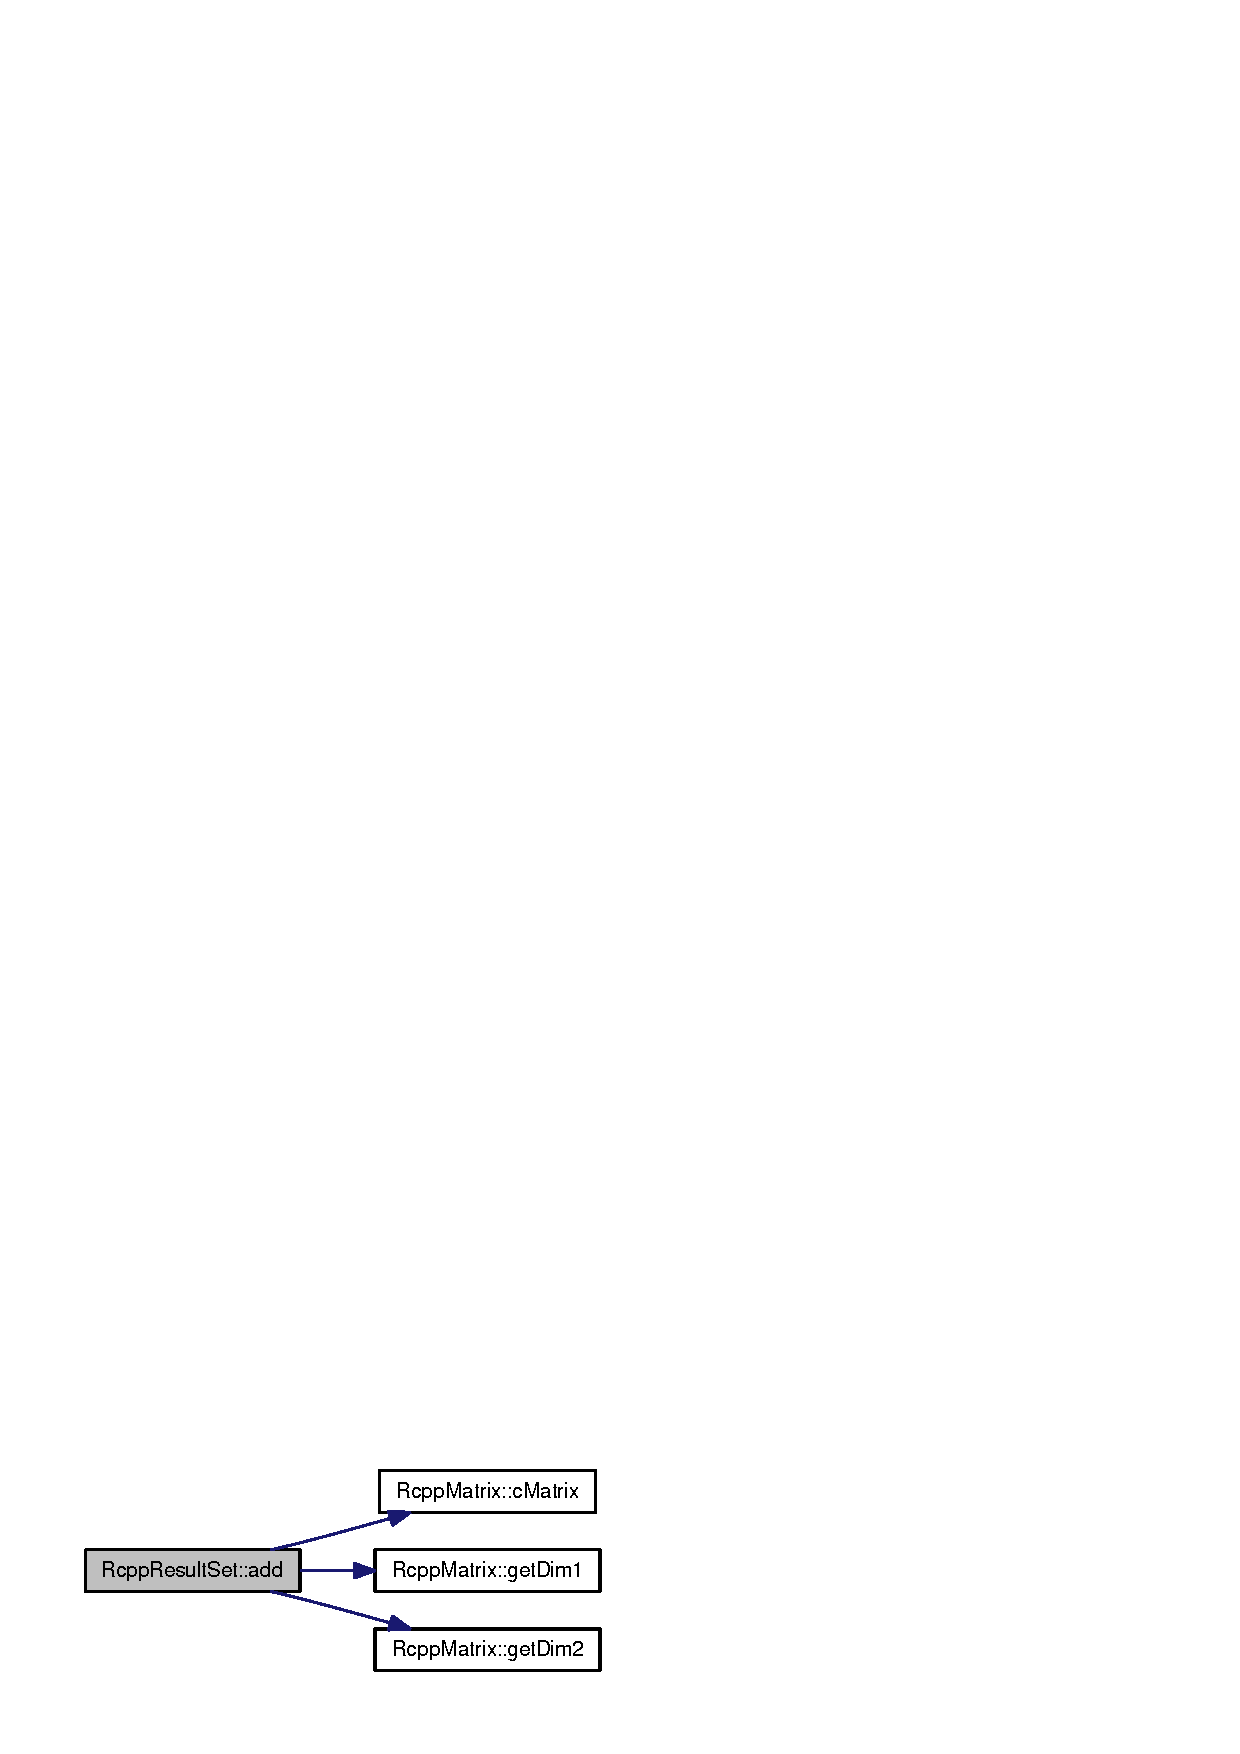
\includegraphics[width=146pt]{classRcppResultSet_f6f50ca0a589fc12ef68c0406e83243b_cgraph}
\end{center}
\end{figure}
\hypertarget{classRcppResultSet_56f1bff720a6cf6503ab942bdb6892b3}{
\index{RcppResultSet@{RcppResultSet}!add@{add}}
\index{add@{add}!RcppResultSet@{RcppResultSet}}
\subsubsection[{add}]{\setlength{\rightskip}{0pt plus 5cm}void RcppResultSet::add (std::string {\em name}, \/  {\bf RcppMatrix}$<$ int $>$ \& {\em mat})}}
\label{classRcppResultSet_56f1bff720a6cf6503ab942bdb6892b3}




Definition at line 672 of file Rcpp.cpp.

References RcppMatrix$<$ T $>$::cMatrix(), RcppMatrix$<$ T $>$::getDim1(), RcppMatrix$<$ T $>$::getDim2(), numProtected, and values.

Here is the call graph for this function:\nopagebreak
\begin{figure}[H]
\begin{center}
\leavevmode
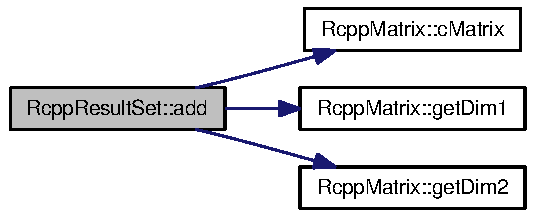
\includegraphics[width=146pt]{classRcppResultSet_56f1bff720a6cf6503ab942bdb6892b3_cgraph}
\end{center}
\end{figure}
\hypertarget{classRcppResultSet_10a64eb042cd3bac5b635670ae2fff5d}{
\index{RcppResultSet@{RcppResultSet}!add@{add}}
\index{add@{add}!RcppResultSet@{RcppResultSet}}
\subsubsection[{add}]{\setlength{\rightskip}{0pt plus 5cm}void RcppResultSet::add (std::string {\em name}, \/  {\bf RcppVector}$<$ double $>$ \& {\em vec})}}
\label{classRcppResultSet_10a64eb042cd3bac5b635670ae2fff5d}




Definition at line 662 of file Rcpp.cpp.

References RcppVector$<$ T $>$::cVector(), numProtected, RcppVector$<$ T $>$::size(), and values.

Here is the call graph for this function:\nopagebreak
\begin{figure}[H]
\begin{center}
\leavevmode
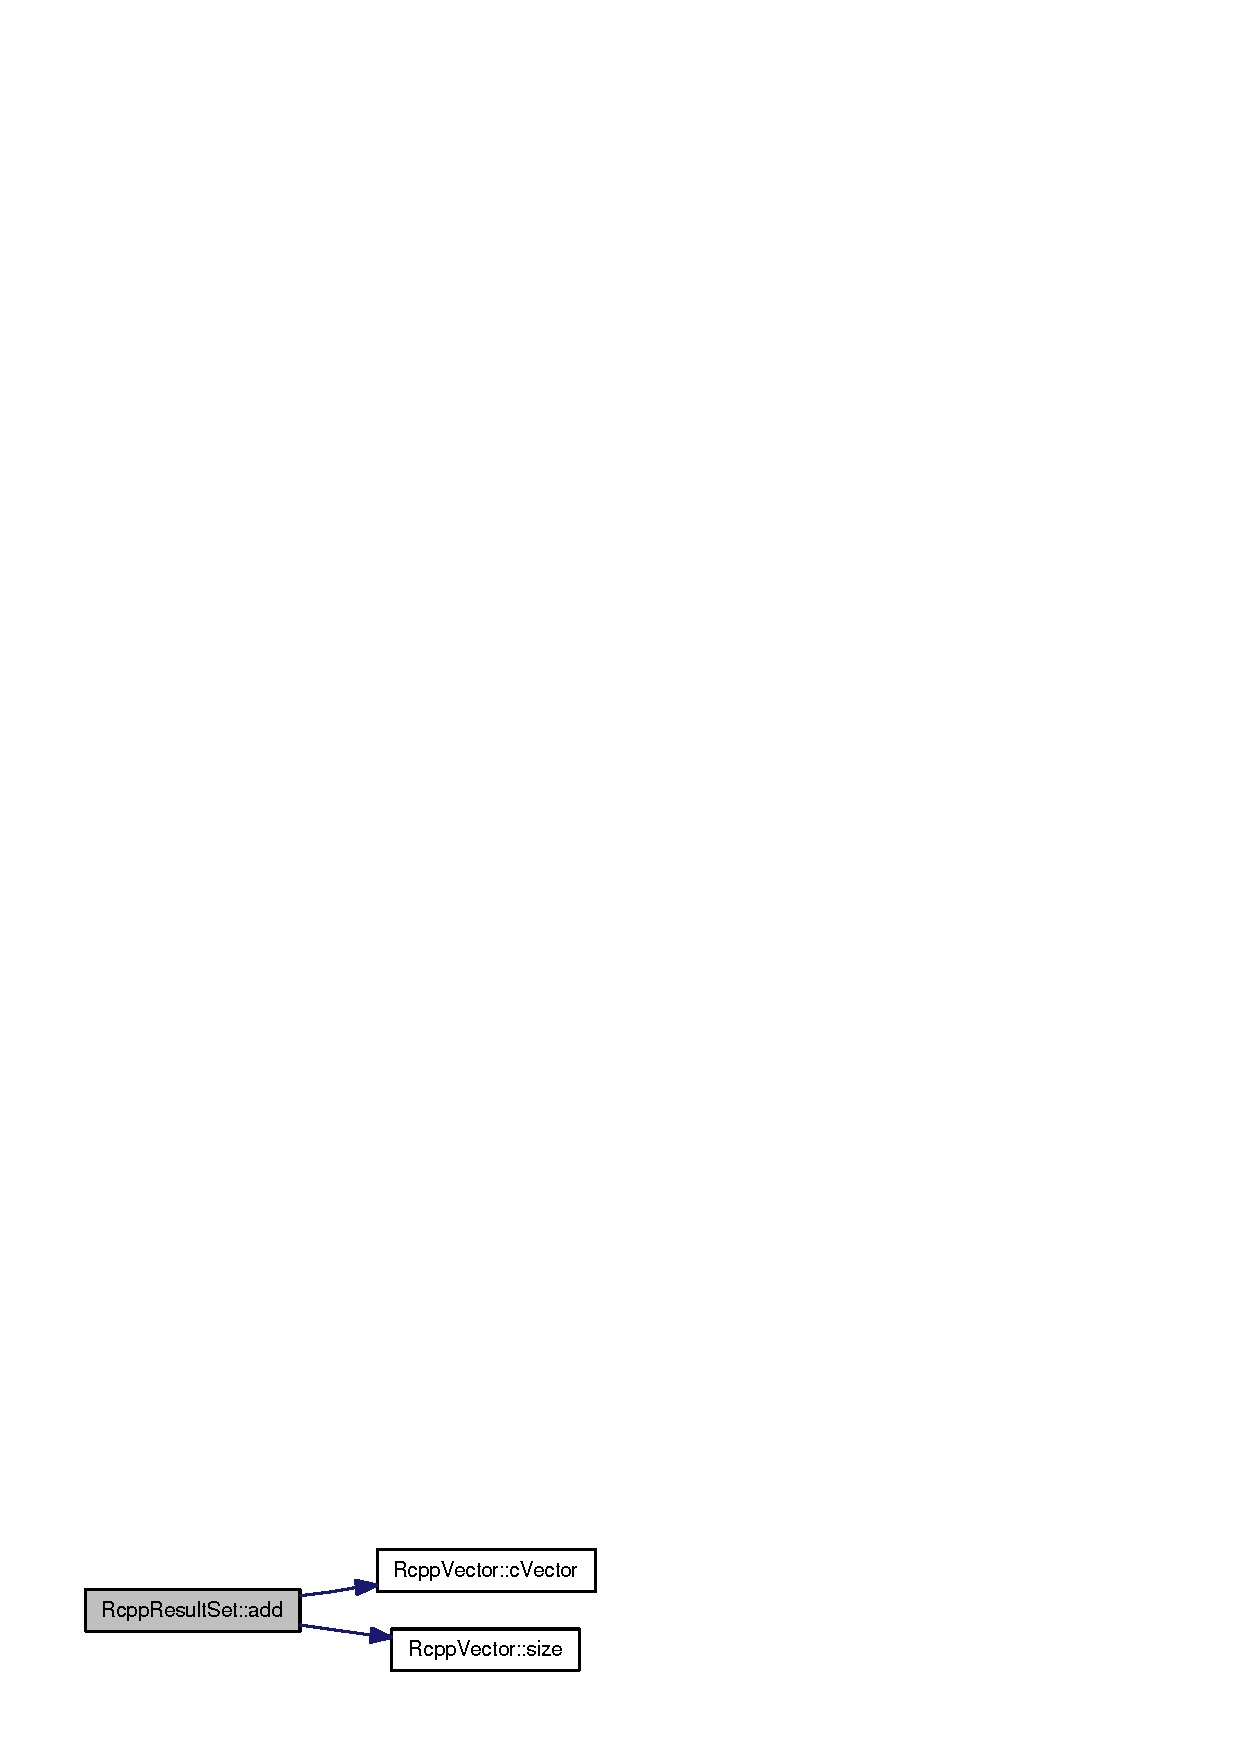
\includegraphics[width=145pt]{classRcppResultSet_10a64eb042cd3bac5b635670ae2fff5d_cgraph}
\end{center}
\end{figure}
\hypertarget{classRcppResultSet_068cb13e27c0e26dd05e92d67eaeb7d0}{
\index{RcppResultSet@{RcppResultSet}!add@{add}}
\index{add@{add}!RcppResultSet@{RcppResultSet}}
\subsubsection[{add}]{\setlength{\rightskip}{0pt plus 5cm}void RcppResultSet::add (std::string {\em name}, \/  {\bf RcppVector}$<$ int $>$ \& {\em vec})}}
\label{classRcppResultSet_068cb13e27c0e26dd05e92d67eaeb7d0}




Definition at line 652 of file Rcpp.cpp.

References RcppVector$<$ T $>$::cVector(), numProtected, RcppVector$<$ T $>$::size(), and values.

Here is the call graph for this function:\nopagebreak
\begin{figure}[H]
\begin{center}
\leavevmode
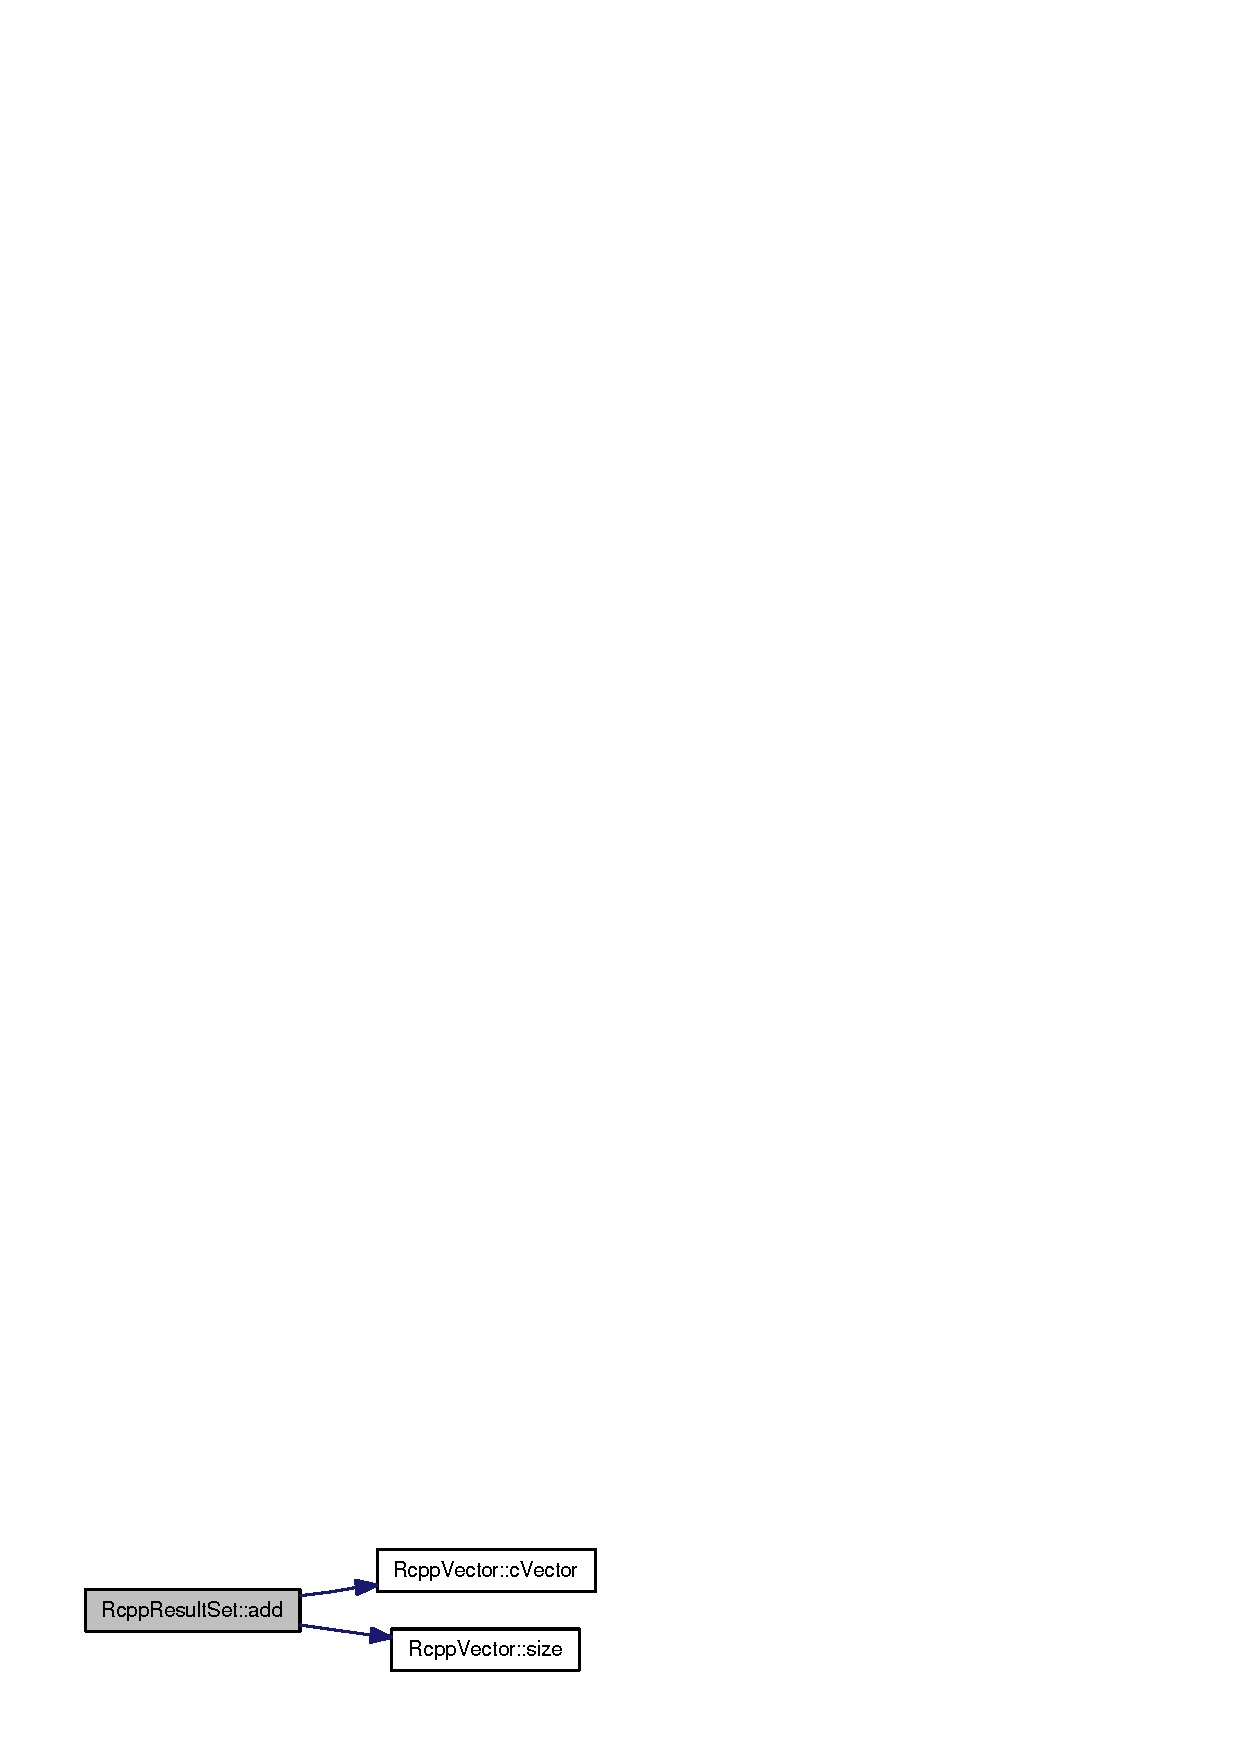
\includegraphics[width=145pt]{classRcppResultSet_068cb13e27c0e26dd05e92d67eaeb7d0_cgraph}
\end{center}
\end{figure}
\hypertarget{classRcppResultSet_db4236a049c8dceb7112229f5e68a295}{
\index{RcppResultSet@{RcppResultSet}!add@{add}}
\index{add@{add}!RcppResultSet@{RcppResultSet}}
\subsubsection[{add}]{\setlength{\rightskip}{0pt plus 5cm}void RcppResultSet::add (std::string {\em name}, \/  std::vector$<$ std::string $>$ \& {\em vec})}}
\label{classRcppResultSet_db4236a049c8dceb7112229f5e68a295}




Definition at line 589 of file Rcpp.cpp.

References numProtected, and values.\hypertarget{classRcppResultSet_b51f30f4bd5f3c6153221a3bd7bb7e24}{
\index{RcppResultSet@{RcppResultSet}!add@{add}}
\index{add@{add}!RcppResultSet@{RcppResultSet}}
\subsubsection[{add}]{\setlength{\rightskip}{0pt plus 5cm}void RcppResultSet::add (std::string {\em name}, \/  std::vector$<$ std::vector$<$ int $>$ $>$ \& {\em mat})}}
\label{classRcppResultSet_b51f30f4bd5f3c6153221a3bd7bb7e24}




Definition at line 622 of file Rcpp.cpp.

References numProtected, and values.\hypertarget{classRcppResultSet_b10cd8503c12708e27068b92a83e4047}{
\index{RcppResultSet@{RcppResultSet}!add@{add}}
\index{add@{add}!RcppResultSet@{RcppResultSet}}
\subsubsection[{add}]{\setlength{\rightskip}{0pt plus 5cm}void RcppResultSet::add (std::string {\em name}, \/  std::vector$<$ std::vector$<$ double $>$ $>$ \& {\em mat})}}
\label{classRcppResultSet_b10cd8503c12708e27068b92a83e4047}




Definition at line 637 of file Rcpp.cpp.

References numProtected, and values.\hypertarget{classRcppResultSet_23fa5be81281adcf3014749094816522}{
\index{RcppResultSet@{RcppResultSet}!add@{add}}
\index{add@{add}!RcppResultSet@{RcppResultSet}}
\subsubsection[{add}]{\setlength{\rightskip}{0pt plus 5cm}void RcppResultSet::add (std::string {\em name}, \/  std::vector$<$ int $>$ \& {\em vec})}}
\label{classRcppResultSet_23fa5be81281adcf3014749094816522}




Definition at line 600 of file Rcpp.cpp.

References numProtected, and values.\hypertarget{classRcppResultSet_2b4575ca5ccc390bc5437b1be4718ca6}{
\index{RcppResultSet@{RcppResultSet}!add@{add}}
\index{add@{add}!RcppResultSet@{RcppResultSet}}
\subsubsection[{add}]{\setlength{\rightskip}{0pt plus 5cm}void RcppResultSet::add (std::string {\em name}, \/  std::vector$<$ double $>$ \& {\em vec})}}
\label{classRcppResultSet_2b4575ca5ccc390bc5437b1be4718ca6}




Definition at line 611 of file Rcpp.cpp.

References numProtected, and values.\hypertarget{classRcppResultSet_10d01a24ef006c1ff14ca7e95fb9e0ea}{
\index{RcppResultSet@{RcppResultSet}!add@{add}}
\index{add@{add}!RcppResultSet@{RcppResultSet}}
\subsubsection[{add}]{\setlength{\rightskip}{0pt plus 5cm}void RcppResultSet::add (std::string {\em name}, \/  {\bf RcppStringVector} \& {\em stringvec})}}
\label{classRcppResultSet_10d01a24ef006c1ff14ca7e95fb9e0ea}




Definition at line 548 of file Rcpp.cpp.

References numProtected, RcppStringVector::size(), and values.

Here is the call graph for this function:\nopagebreak
\begin{figure}[H]
\begin{center}
\leavevmode
\includegraphics[width=150pt]{classRcppResultSet_10d01a24ef006c1ff14ca7e95fb9e0ea_cgraph}
\end{center}
\end{figure}
\hypertarget{classRcppResultSet_ac8cade970247a377e8dbebf1c79a86c}{
\index{RcppResultSet@{RcppResultSet}!add@{add}}
\index{add@{add}!RcppResultSet@{RcppResultSet}}
\subsubsection[{add}]{\setlength{\rightskip}{0pt plus 5cm}void RcppResultSet::add (std::string {\em name}, \/  {\bf RcppDatetimeVector} \& {\em dtvec})}}
\label{classRcppResultSet_ac8cade970247a377e8dbebf1c79a86c}




Definition at line 534 of file Rcpp.cpp.

References numProtected, RcppDatetimeVector::size(), and values.

Here is the call graph for this function:\nopagebreak
\begin{figure}[H]
\begin{center}
\leavevmode
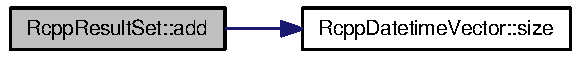
\includegraphics[width=157pt]{classRcppResultSet_ac8cade970247a377e8dbebf1c79a86c_cgraph}
\end{center}
\end{figure}
\hypertarget{classRcppResultSet_1d921e7a24e50369ae67a1bc63826131}{
\index{RcppResultSet@{RcppResultSet}!add@{add}}
\index{add@{add}!RcppResultSet@{RcppResultSet}}
\subsubsection[{add}]{\setlength{\rightskip}{0pt plus 5cm}void RcppResultSet::add (std::string {\em name}, \/  {\bf RcppDatetime} \& {\em datetime})}}
\label{classRcppResultSet_1d921e7a24e50369ae67a1bc63826131}




Definition at line 478 of file Rcpp.cpp.

References RcppDatetime::getFractionalTimestamp(), numProtected, and values.

Here is the call graph for this function:\nopagebreak
\begin{figure}[H]
\begin{center}
\leavevmode
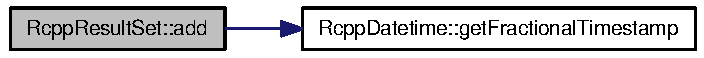
\includegraphics[width=187pt]{classRcppResultSet_1d921e7a24e50369ae67a1bc63826131_cgraph}
\end{center}
\end{figure}
\hypertarget{classRcppResultSet_d7efd746596959ce68ca98c690a2f645}{
\index{RcppResultSet@{RcppResultSet}!add@{add}}
\index{add@{add}!RcppResultSet@{RcppResultSet}}
\subsubsection[{add}]{\setlength{\rightskip}{0pt plus 5cm}void RcppResultSet::add (std::string {\em name}, \/  {\bf RcppDateVector} \& {\em datevec})}}
\label{classRcppResultSet_d7efd746596959ce68ca98c690a2f645}




Definition at line 521 of file Rcpp.cpp.

References RcppDate::Jan1970Offset, numProtected, RcppDateVector::size(), and values.

Here is the call graph for this function:\nopagebreak
\begin{figure}[H]
\begin{center}
\leavevmode
\includegraphics[width=148pt]{classRcppResultSet_d7efd746596959ce68ca98c690a2f645_cgraph}
\end{center}
\end{figure}
\hypertarget{classRcppResultSet_e5cb861a0d6e95cc7ed465ccae2ac4a7}{
\index{RcppResultSet@{RcppResultSet}!add@{add}}
\index{add@{add}!RcppResultSet@{RcppResultSet}}
\subsubsection[{add}]{\setlength{\rightskip}{0pt plus 5cm}void RcppResultSet::add (std::string {\em name}, \/  {\bf RcppDate} \& {\em date})}}
\label{classRcppResultSet_e5cb861a0d6e95cc7ed465ccae2ac4a7}




Definition at line 467 of file Rcpp.cpp.

References RcppDate::getJDN(), RcppDate::Jan1970Offset, numProtected, and values.

Here is the call graph for this function:\nopagebreak
\begin{figure}[H]
\begin{center}
\leavevmode
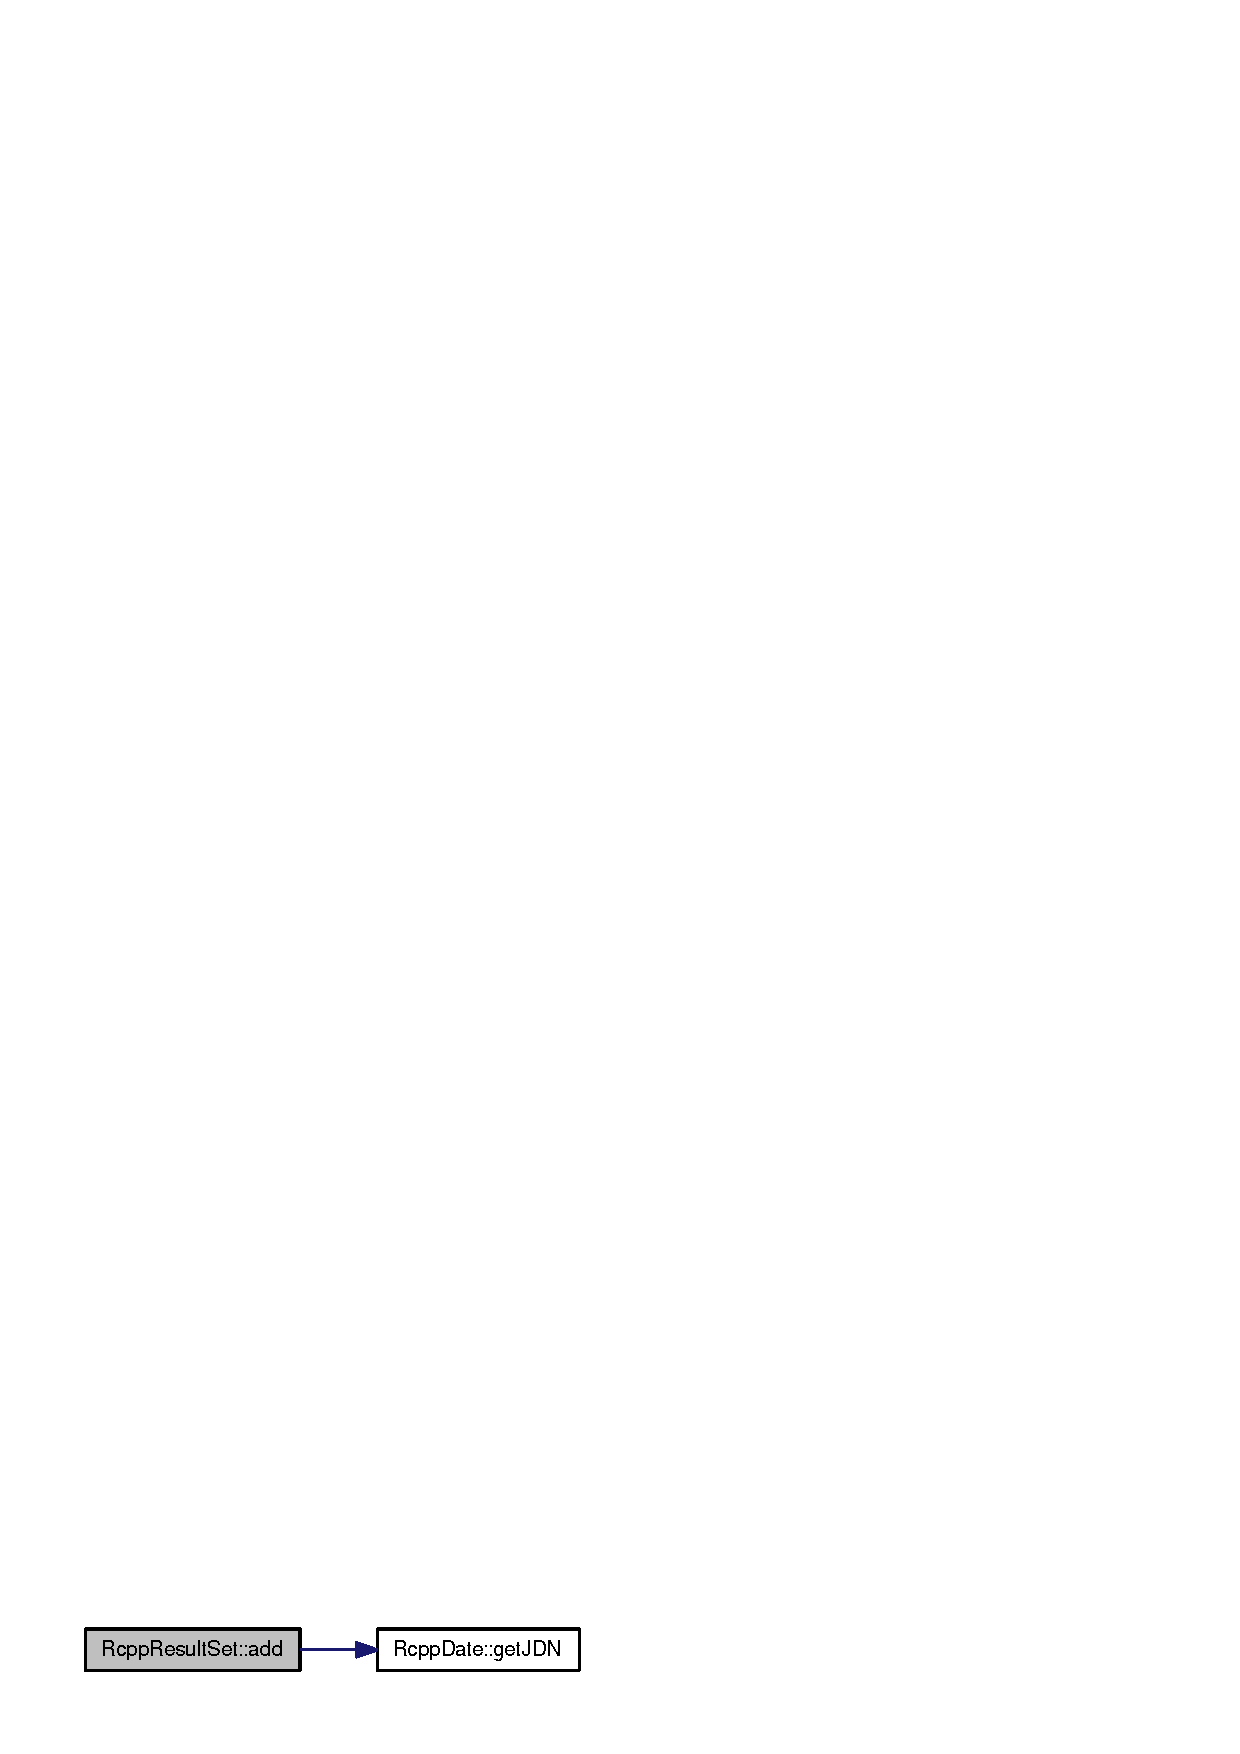
\includegraphics[width=141pt]{classRcppResultSet_e5cb861a0d6e95cc7ed465ccae2ac4a7_cgraph}
\end{center}
\end{figure}
\hypertarget{classRcppResultSet_2cca9ea4e9554c4fad9bc326355c354c}{
\index{RcppResultSet@{RcppResultSet}!add@{add}}
\index{add@{add}!RcppResultSet@{RcppResultSet}}
\subsubsection[{add}]{\setlength{\rightskip}{0pt plus 5cm}void RcppResultSet::add (std::string {\em name}, \/  int $\ast$$\ast$ {\em mat}, \/  int {\em nx}, \/  int {\em ny})}}
\label{classRcppResultSet_2cca9ea4e9554c4fad9bc326355c354c}




Definition at line 578 of file Rcpp.cpp.

References numProtected, and values.\hypertarget{classRcppResultSet_88ff0e3db486eec0012eb58beee05e9b}{
\index{RcppResultSet@{RcppResultSet}!add@{add}}
\index{add@{add}!RcppResultSet@{RcppResultSet}}
\subsubsection[{add}]{\setlength{\rightskip}{0pt plus 5cm}void RcppResultSet::add (std::string {\em name}, \/  double $\ast$$\ast$ {\em mat}, \/  int {\em nx}, \/  int {\em ny})}}
\label{classRcppResultSet_88ff0e3db486eec0012eb58beee05e9b}




Definition at line 567 of file Rcpp.cpp.

References numProtected, and values.\hypertarget{classRcppResultSet_494dbe1f6db48bf48e9e33a32d897f29}{
\index{RcppResultSet@{RcppResultSet}!add@{add}}
\index{add@{add}!RcppResultSet@{RcppResultSet}}
\subsubsection[{add}]{\setlength{\rightskip}{0pt plus 5cm}void RcppResultSet::add (std::string {\em name}, \/  int $\ast$ {\em vec}, \/  int {\em len})}}
\label{classRcppResultSet_494dbe1f6db48bf48e9e33a32d897f29}




Definition at line 557 of file Rcpp.cpp.

References numProtected, and values.\hypertarget{classRcppResultSet_5d06d8a4f0497abc6fad4ea22b4934f9}{
\index{RcppResultSet@{RcppResultSet}!add@{add}}
\index{add@{add}!RcppResultSet@{RcppResultSet}}
\subsubsection[{add}]{\setlength{\rightskip}{0pt plus 5cm}void RcppResultSet::add (std::string {\em name}, \/  double $\ast$ {\em vec}, \/  int {\em len})}}
\label{classRcppResultSet_5d06d8a4f0497abc6fad4ea22b4934f9}




Definition at line 511 of file Rcpp.cpp.

References numProtected, and values.\hypertarget{classRcppResultSet_2633372ab2f50b269e9e26dd7a489492}{
\index{RcppResultSet@{RcppResultSet}!add@{add}}
\index{add@{add}!RcppResultSet@{RcppResultSet}}
\subsubsection[{add}]{\setlength{\rightskip}{0pt plus 5cm}void RcppResultSet::add (std::string {\em name}, \/  std::string {\em strvalue})}}
\label{classRcppResultSet_2633372ab2f50b269e9e26dd7a489492}




Definition at line 504 of file Rcpp.cpp.

References numProtected, and values.\hypertarget{classRcppResultSet_8b7841ff8a52477b0c6a1fb7c03c0fd9}{
\index{RcppResultSet@{RcppResultSet}!add@{add}}
\index{add@{add}!RcppResultSet@{RcppResultSet}}
\subsubsection[{add}]{\setlength{\rightskip}{0pt plus 5cm}void RcppResultSet::add (std::string {\em name}, \/  int {\em i})}}
\label{classRcppResultSet_8b7841ff8a52477b0c6a1fb7c03c0fd9}




Definition at line 497 of file Rcpp.cpp.

References numProtected, and values.\hypertarget{classRcppResultSet_7c7da37f18bd352303bf06b7c5233bc4}{
\index{RcppResultSet@{RcppResultSet}!add@{add}}
\index{add@{add}!RcppResultSet@{RcppResultSet}}
\subsubsection[{add}]{\setlength{\rightskip}{0pt plus 5cm}void RcppResultSet::add (std::string {\em name}, \/  double {\em x})}}
\label{classRcppResultSet_7c7da37f18bd352303bf06b7c5233bc4}




Definition at line 490 of file Rcpp.cpp.

References numProtected, and values.

Referenced by Rcpp\_\-Example(), RcppDateExample(), and RcppVectorExample().\hypertarget{classRcppResultSet_916989ff6c0ed1149a5f93fb6a532946}{
\index{RcppResultSet@{RcppResultSet}!getReturnList@{getReturnList}}
\index{getReturnList@{getReturnList}!RcppResultSet@{RcppResultSet}}
\subsubsection[{getReturnList}]{\setlength{\rightskip}{0pt plus 5cm}SEXP RcppResultSet::getReturnList ()}}
\label{classRcppResultSet_916989ff6c0ed1149a5f93fb6a532946}




Definition at line 784 of file Rcpp.cpp.

References numProtected, and values.

Referenced by Rcpp\_\-Example(), RcppDateExample(), and RcppVectorExample().

\subsection{Member Data Documentation}
\hypertarget{classRcppResultSet_19edd02ac05783f9b4fd840c22e74153}{
\index{RcppResultSet@{RcppResultSet}!numProtected@{numProtected}}
\index{numProtected@{numProtected}!RcppResultSet@{RcppResultSet}}
\subsubsection[{numProtected}]{\setlength{\rightskip}{0pt plus 5cm}int {\bf RcppResultSet::numProtected}\hspace{0.3cm}{\tt  \mbox{[}protected\mbox{]}}}}
\label{classRcppResultSet_19edd02ac05783f9b4fd840c22e74153}




Definition at line 586 of file Rcpp.h.

Referenced by add(), getReturnList(), and RcppResultSet().\hypertarget{classRcppResultSet_509f3d779c88476dea89ade9c08d403f}{
\index{RcppResultSet@{RcppResultSet}!values@{values}}
\index{values@{values}!RcppResultSet@{RcppResultSet}}
\subsubsection[{values}]{\setlength{\rightskip}{0pt plus 5cm}std::list$<$std::pair$<$std::string,SEXP$>$ $>$ {\bf RcppResultSet::values}\hspace{0.3cm}{\tt  \mbox{[}protected\mbox{]}}}}
\label{classRcppResultSet_509f3d779c88476dea89ade9c08d403f}




Definition at line 587 of file Rcpp.h.

Referenced by add(), and getReturnList().

The documentation for this class was generated from the following files:\begin{CompactItemize}
\item 
src/\hyperlink{Rcpp_8h}{Rcpp.h}\item 
src/\hyperlink{Rcpp_8cpp}{Rcpp.cpp}\end{CompactItemize}

\hypertarget{classRcppStringVector}{
\section{RcppStringVector Class Reference}
\label{classRcppStringVector}\index{RcppStringVector@{RcppStringVector}}
}


{\ttfamily \#include $<$Rcpp.h$>$}\subsection*{Public Member Functions}
\begin{DoxyCompactItemize}
\item 
\hyperlink{classRcppStringVector_af0216e26ab72efb7a6b07182224f84c5}{RcppStringVector} (SEXP vec)
\item 
\hyperlink{classRcppStringVector_a1b0550e206ac6945b00ee02c3c4bf373}{$\sim$RcppStringVector} ()
\item 
std::string \& \hyperlink{classRcppStringVector_aea5aa96f98f1c5b21e3c56ff60c7c413}{operator()} (int i)
\item 
int \hyperlink{classRcppStringVector_ac52a8eb61411546a62a70636709b1172}{size} ()
\item 
std::vector$<$ std::string $>$ \hyperlink{classRcppStringVector_a2bd817c9332e1446ddf034938b256cc3}{stlVector} ()
\end{DoxyCompactItemize}
\subsection*{Private Attributes}
\begin{DoxyCompactItemize}
\item 
std::string $\ast$ \hyperlink{classRcppStringVector_a94d14fa5093cc8219cbcb91aadfed09e}{v}
\item 
int \hyperlink{classRcppStringVector_aaa2e2e4335d14e46fc96b07836e99573}{length}
\end{DoxyCompactItemize}


\subsection{Detailed Description}


Definition at line 380 of file Rcpp.h.

\subsection{Constructor \& Destructor Documentation}
\hypertarget{classRcppStringVector_af0216e26ab72efb7a6b07182224f84c5}{
\index{RcppStringVector@{RcppStringVector}!RcppStringVector@{RcppStringVector}}
\index{RcppStringVector@{RcppStringVector}!RcppStringVector@{RcppStringVector}}
\subsubsection[{RcppStringVector}]{\setlength{\rightskip}{0pt plus 5cm}RcppStringVector::RcppStringVector (SEXP {\em vec})}}
\label{classRcppStringVector_af0216e26ab72efb7a6b07182224f84c5}


Definition at line 283 of file Rcpp.cpp.

References length, and v.\hypertarget{classRcppStringVector_a1b0550e206ac6945b00ee02c3c4bf373}{
\index{RcppStringVector@{RcppStringVector}!$\sim$RcppStringVector@{$\sim$RcppStringVector}}
\index{$\sim$RcppStringVector@{$\sim$RcppStringVector}!RcppStringVector@{RcppStringVector}}
\subsubsection[{$\sim$RcppStringVector}]{\setlength{\rightskip}{0pt plus 5cm}RcppStringVector::$\sim$RcppStringVector ()\hspace{0.3cm}{\ttfamily  \mbox{[}inline\mbox{]}}}}
\label{classRcppStringVector_a1b0550e206ac6945b00ee02c3c4bf373}


Definition at line 383 of file Rcpp.h.

References v.

\subsection{Member Function Documentation}
\hypertarget{classRcppStringVector_aea5aa96f98f1c5b21e3c56ff60c7c413}{
\index{RcppStringVector@{RcppStringVector}!operator()@{operator()}}
\index{operator()@{operator()}!RcppStringVector@{RcppStringVector}}
\subsubsection[{operator()}]{\setlength{\rightskip}{0pt plus 5cm}std::string\& RcppStringVector::operator() (int {\em i})\hspace{0.3cm}{\ttfamily  \mbox{[}inline\mbox{]}}}}
\label{classRcppStringVector_aea5aa96f98f1c5b21e3c56ff60c7c413}


Definition at line 386 of file Rcpp.h.

References length, and v.\hypertarget{classRcppStringVector_ac52a8eb61411546a62a70636709b1172}{
\index{RcppStringVector@{RcppStringVector}!size@{size}}
\index{size@{size}!RcppStringVector@{RcppStringVector}}
\subsubsection[{size}]{\setlength{\rightskip}{0pt plus 5cm}int RcppStringVector::size ()\hspace{0.3cm}{\ttfamily  \mbox{[}inline\mbox{]}}}}
\label{classRcppStringVector_ac52a8eb61411546a62a70636709b1172}


Definition at line 394 of file Rcpp.h.

References length.

Referenced by RcppResultSet::add().\hypertarget{classRcppStringVector_a2bd817c9332e1446ddf034938b256cc3}{
\index{RcppStringVector@{RcppStringVector}!stlVector@{stlVector}}
\index{stlVector@{stlVector}!RcppStringVector@{RcppStringVector}}
\subsubsection[{stlVector}]{\setlength{\rightskip}{0pt plus 5cm}std::vector$<$std::string$>$ RcppStringVector::stlVector ()\hspace{0.3cm}{\ttfamily  \mbox{[}inline\mbox{]}}}}
\label{classRcppStringVector_a2bd817c9332e1446ddf034938b256cc3}


Definition at line 395 of file Rcpp.h.

References length, and v.

\subsection{Member Data Documentation}
\hypertarget{classRcppStringVector_aaa2e2e4335d14e46fc96b07836e99573}{
\index{RcppStringVector@{RcppStringVector}!length@{length}}
\index{length@{length}!RcppStringVector@{RcppStringVector}}
\subsubsection[{length}]{\setlength{\rightskip}{0pt plus 5cm}int {\bf RcppStringVector::length}\hspace{0.3cm}{\ttfamily  \mbox{[}private\mbox{]}}}}
\label{classRcppStringVector_aaa2e2e4335d14e46fc96b07836e99573}


Definition at line 403 of file Rcpp.h.

Referenced by operator()(), RcppStringVector(), size(), and stlVector().\hypertarget{classRcppStringVector_a94d14fa5093cc8219cbcb91aadfed09e}{
\index{RcppStringVector@{RcppStringVector}!v@{v}}
\index{v@{v}!RcppStringVector@{RcppStringVector}}
\subsubsection[{v}]{\setlength{\rightskip}{0pt plus 5cm}std::string$\ast$ {\bf RcppStringVector::v}\hspace{0.3cm}{\ttfamily  \mbox{[}private\mbox{]}}}}
\label{classRcppStringVector_a94d14fa5093cc8219cbcb91aadfed09e}


Definition at line 402 of file Rcpp.h.

Referenced by operator()(), RcppStringVector(), stlVector(), and $\sim$RcppStringVector().

The documentation for this class was generated from the following files:\begin{DoxyCompactItemize}
\item 
src/\hyperlink{Rcpp_8h}{Rcpp.h}\item 
src/\hyperlink{Rcpp_8cpp}{Rcpp.cpp}\end{DoxyCompactItemize}

\hypertarget{classRcppStringVectorView}{
\section{RcppStringVectorView Class Reference}
\label{classRcppStringVectorView}\index{RcppStringVectorView@{RcppStringVectorView}}
}
{\tt \#include $<$Rcpp.h$>$}

\subsection*{Public Member Functions}
\begin{CompactItemize}
\item 
\hyperlink{classRcppStringVectorView_c74085bb16d7a13b58eb59f69268ec85}{RcppStringVectorView} (SEXP vec)
\item 
const char $\ast$ \hyperlink{classRcppStringVectorView_b81899b7d6c595f84d2fb07809ff002c}{operator()} (int i)
\item 
int \hyperlink{classRcppStringVectorView_df0f6b6541339ca747c4ed79c445869e}{size} ()
\end{CompactItemize}
\subsection*{Private Attributes}
\begin{CompactItemize}
\item 
SEXP \hyperlink{classRcppStringVectorView_1db3cc1a2dd1809151351c123343c15e}{v}
\item 
int \hyperlink{classRcppStringVectorView_ef6edaa52c234b4bb1fd1fc949fa0f25}{length}
\end{CompactItemize}


\subsection{Detailed Description}


Definition at line 506 of file Rcpp.h.

\subsection{Constructor \& Destructor Documentation}
\hypertarget{classRcppStringVectorView_c74085bb16d7a13b58eb59f69268ec85}{
\index{RcppStringVectorView@{RcppStringVectorView}!RcppStringVectorView@{RcppStringVectorView}}
\index{RcppStringVectorView@{RcppStringVectorView}!RcppStringVectorView@{RcppStringVectorView}}
\subsubsection[RcppStringVectorView]{\setlength{\rightskip}{0pt plus 5cm}RcppStringVectorView::RcppStringVectorView (SEXP {\em vec})}}
\label{classRcppStringVectorView_c74085bb16d7a13b58eb59f69268ec85}




Definition at line 441 of file Rcpp.cpp.

References length, and v.

\subsection{Member Function Documentation}
\hypertarget{classRcppStringVectorView_b81899b7d6c595f84d2fb07809ff002c}{
\index{RcppStringVectorView@{RcppStringVectorView}!operator()@{operator()}}
\index{operator()@{operator()}!RcppStringVectorView@{RcppStringVectorView}}
\subsubsection[operator()]{\setlength{\rightskip}{0pt plus 5cm}const char$\ast$ RcppStringVectorView::operator() (int {\em i})\hspace{0.3cm}{\tt  \mbox{[}inline\mbox{]}}}}
\label{classRcppStringVectorView_b81899b7d6c595f84d2fb07809ff002c}




Definition at line 509 of file Rcpp.h.

References length, and v.\hypertarget{classRcppStringVectorView_df0f6b6541339ca747c4ed79c445869e}{
\index{RcppStringVectorView@{RcppStringVectorView}!size@{size}}
\index{size@{size}!RcppStringVectorView@{RcppStringVectorView}}
\subsubsection[size]{\setlength{\rightskip}{0pt plus 5cm}int RcppStringVectorView::size ()\hspace{0.3cm}{\tt  \mbox{[}inline\mbox{]}}}}
\label{classRcppStringVectorView_df0f6b6541339ca747c4ed79c445869e}




Definition at line 517 of file Rcpp.h.

References length.

\subsection{Member Data Documentation}
\hypertarget{classRcppStringVectorView_1db3cc1a2dd1809151351c123343c15e}{
\index{RcppStringVectorView@{RcppStringVectorView}!v@{v}}
\index{v@{v}!RcppStringVectorView@{RcppStringVectorView}}
\subsubsection[v]{\setlength{\rightskip}{0pt plus 5cm}SEXP {\bf RcppStringVectorView::v}\hspace{0.3cm}{\tt  \mbox{[}private\mbox{]}}}}
\label{classRcppStringVectorView_1db3cc1a2dd1809151351c123343c15e}




Definition at line 519 of file Rcpp.h.

Referenced by operator()(), and RcppStringVectorView().\hypertarget{classRcppStringVectorView_ef6edaa52c234b4bb1fd1fc949fa0f25}{
\index{RcppStringVectorView@{RcppStringVectorView}!length@{length}}
\index{length@{length}!RcppStringVectorView@{RcppStringVectorView}}
\subsubsection[length]{\setlength{\rightskip}{0pt plus 5cm}int {\bf RcppStringVectorView::length}\hspace{0.3cm}{\tt  \mbox{[}private\mbox{]}}}}
\label{classRcppStringVectorView_ef6edaa52c234b4bb1fd1fc949fa0f25}




Definition at line 520 of file Rcpp.h.

Referenced by operator()(), RcppStringVectorView(), and size().

The documentation for this class was generated from the following files:\begin{CompactItemize}
\item 
src/\hyperlink{Rcpp_8h}{Rcpp.h}\item 
src/\hyperlink{Rcpp_8cpp}{Rcpp.cpp}\end{CompactItemize}

\hypertarget{classRcppVector}{
\section{RcppVector$<$ T $>$ Class Template Reference}
\label{classRcppVector}\index{RcppVector@{RcppVector}}
}
{\tt \#include $<$Rcpp.h$>$}

Collaboration diagram for RcppVector$<$ T $>$:\nopagebreak
\begin{figure}[H]
\begin{center}
\leavevmode
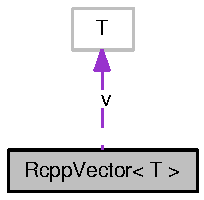
\includegraphics[width=67pt]{classRcppVector__coll__graph}
\end{center}
\end{figure}
\subsection*{Public Member Functions}
\begin{CompactItemize}
\item 
\hyperlink{classRcppVector_0925b350f636a546e58ad0329786500a}{RcppVector} (SEXP vec)
\item 
\hyperlink{classRcppVector_eb7797ca2b2ac2d03fee0a543993f17b}{RcppVector} (int \hyperlink{classRcppVector_733f5ed23ade0723338904f9f08457d6}{len})
\item 
int \hyperlink{classRcppVector_1e2424dc9b91014ba8b2c9351d97eb37}{size} ()
\item 
T \& \hyperlink{classRcppVector_66aca1da0563af28e55768d98488a42d}{operator()} (int i)
\item 
T $\ast$ \hyperlink{classRcppVector_f4660a27a888a51693b02d2f51b47b08}{cVector} ()
\item 
std::vector$<$ T $>$ \hyperlink{classRcppVector_c650f89b966962b167f3bc42aecf213b}{stlVector} ()
\end{CompactItemize}
\subsection*{Private Attributes}
\begin{CompactItemize}
\item 
int \hyperlink{classRcppVector_733f5ed23ade0723338904f9f08457d6}{len}
\item 
T $\ast$ \hyperlink{classRcppVector_c810c53db4c1b978bada104b38484b26}{v}
\end{CompactItemize}


\subsection{Detailed Description}
\subsubsection*{template$<$typename T$>$ class RcppVector$<$ T $>$}



Definition at line 358 of file Rcpp.h.

\subsection{Constructor \& Destructor Documentation}
\hypertarget{classRcppVector_0925b350f636a546e58ad0329786500a}{
\index{RcppVector@{RcppVector}!RcppVector@{RcppVector}}
\index{RcppVector@{RcppVector}!RcppVector@{RcppVector}}
\subsubsection[RcppVector]{\setlength{\rightskip}{0pt plus 5cm}template$<$typename T$>$ {\bf RcppVector}$<$ T $>$::{\bf RcppVector} (SEXP {\em vec})\hspace{0.3cm}{\tt  \mbox{[}inline\mbox{]}}}}
\label{classRcppVector_0925b350f636a546e58ad0329786500a}




Definition at line 290 of file Rcpp.cpp.

References RcppVector$<$ T $>$::len, and RcppVector$<$ T $>$::v.\hypertarget{classRcppVector_eb7797ca2b2ac2d03fee0a543993f17b}{
\index{RcppVector@{RcppVector}!RcppVector@{RcppVector}}
\index{RcppVector@{RcppVector}!RcppVector@{RcppVector}}
\subsubsection[RcppVector]{\setlength{\rightskip}{0pt plus 5cm}template$<$typename T$>$ {\bf RcppVector}$<$ T $>$::{\bf RcppVector} (int {\em len})\hspace{0.3cm}{\tt  \mbox{[}inline\mbox{]}}}}
\label{classRcppVector_eb7797ca2b2ac2d03fee0a543993f17b}




Definition at line 314 of file Rcpp.cpp.

References RcppVector$<$ T $>$::len, and RcppVector$<$ T $>$::v.

\subsection{Member Function Documentation}
\hypertarget{classRcppVector_1e2424dc9b91014ba8b2c9351d97eb37}{
\index{RcppVector@{RcppVector}!size@{size}}
\index{size@{size}!RcppVector@{RcppVector}}
\subsubsection[size]{\setlength{\rightskip}{0pt plus 5cm}template$<$typename T$>$ int {\bf RcppVector}$<$ T $>$::size ()\hspace{0.3cm}{\tt  \mbox{[}inline\mbox{]}}}}
\label{classRcppVector_1e2424dc9b91014ba8b2c9351d97eb37}




Definition at line 362 of file Rcpp.h.

Referenced by RcppResultSet::add(), Rcpp\_\-Example(), and RcppVectorExample().\hypertarget{classRcppVector_66aca1da0563af28e55768d98488a42d}{
\index{RcppVector@{RcppVector}!operator()@{operator()}}
\index{operator()@{operator()}!RcppVector@{RcppVector}}
\subsubsection[operator()]{\setlength{\rightskip}{0pt plus 5cm}template$<$typename T$>$ T\& {\bf RcppVector}$<$ T $>$::operator() (int {\em i})\hspace{0.3cm}{\tt  \mbox{[}inline\mbox{]}}}}
\label{classRcppVector_66aca1da0563af28e55768d98488a42d}




Definition at line 363 of file Rcpp.h.

References RcppVector$<$ T $>$::v.\hypertarget{classRcppVector_f4660a27a888a51693b02d2f51b47b08}{
\index{RcppVector@{RcppVector}!cVector@{cVector}}
\index{cVector@{cVector}!RcppVector@{RcppVector}}
\subsubsection[cVector]{\setlength{\rightskip}{0pt plus 5cm}template$<$typename T$>$ T $\ast$ {\bf RcppVector}$<$ T $>$::cVector ()\hspace{0.3cm}{\tt  \mbox{[}inline\mbox{]}}}}
\label{classRcppVector_f4660a27a888a51693b02d2f51b47b08}




Definition at line 322 of file Rcpp.cpp.

References RcppVector$<$ T $>$::len, and RcppVector$<$ T $>$::v.

Referenced by RcppResultSet::add(), and Rcpp\_\-Example().\hypertarget{classRcppVector_c650f89b966962b167f3bc42aecf213b}{
\index{RcppVector@{RcppVector}!stlVector@{stlVector}}
\index{stlVector@{stlVector}!RcppVector@{RcppVector}}
\subsubsection[stlVector]{\setlength{\rightskip}{0pt plus 5cm}template$<$typename T$>$ std::vector$<$ T $>$ {\bf RcppVector}$<$ T $>$::stlVector ()\hspace{0.3cm}{\tt  \mbox{[}inline\mbox{]}}}}
\label{classRcppVector_c650f89b966962b167f3bc42aecf213b}




Definition at line 330 of file Rcpp.cpp.

References RcppVector$<$ T $>$::len, and RcppVector$<$ T $>$::v.

Referenced by Rcpp\_\-Example().

\subsection{Member Data Documentation}
\hypertarget{classRcppVector_733f5ed23ade0723338904f9f08457d6}{
\index{RcppVector@{RcppVector}!len@{len}}
\index{len@{len}!RcppVector@{RcppVector}}
\subsubsection[len]{\setlength{\rightskip}{0pt plus 5cm}template$<$typename T$>$ int {\bf RcppVector}$<$ T $>$::{\bf len}\hspace{0.3cm}{\tt  \mbox{[}private\mbox{]}}}}
\label{classRcppVector_733f5ed23ade0723338904f9f08457d6}




Definition at line 374 of file Rcpp.h.

Referenced by RcppVector$<$ T $>$::cVector(), RcppVector$<$ T $>$::RcppVector(), and RcppVector$<$ T $>$::stlVector().\hypertarget{classRcppVector_c810c53db4c1b978bada104b38484b26}{
\index{RcppVector@{RcppVector}!v@{v}}
\index{v@{v}!RcppVector@{RcppVector}}
\subsubsection[v]{\setlength{\rightskip}{0pt plus 5cm}template$<$typename T$>$ T$\ast$ {\bf RcppVector}$<$ T $>$::{\bf v}\hspace{0.3cm}{\tt  \mbox{[}private\mbox{]}}}}
\label{classRcppVector_c810c53db4c1b978bada104b38484b26}




Definition at line 375 of file Rcpp.h.

Referenced by RcppVector$<$ T $>$::cVector(), RcppVector$<$ T $>$::operator()(), RcppVector$<$ T $>$::RcppVector(), and RcppVector$<$ T $>$::stlVector().

The documentation for this class was generated from the following files:\begin{CompactItemize}
\item 
src/\hyperlink{Rcpp_8h}{Rcpp.h}\item 
src/\hyperlink{Rcpp_8cpp}{Rcpp.cpp}\end{CompactItemize}

\hypertarget{classRcppVectorView}{
\section{RcppVectorView$<$ T $>$ Class Template Reference}
\label{classRcppVectorView}\index{RcppVectorView@{RcppVectorView}}
}
{\tt \#include $<$Rcpp.h$>$}

\subsection*{Public Member Functions}
\begin{CompactItemize}
\item 
\hyperlink{classRcppVectorView_d2e90fed8ee8a40f56591cc94f83041e}{RcppVectorView} (SEXP vec)
\item 
int \hyperlink{classRcppVectorView_d4c0f21296eb1cf7b2e2c8b8b43f4b0d}{size} () const 
\item 
T \hyperlink{classRcppVectorView_13d63e990363a37ae29e0eab7400d297}{operator()} (int i) const 
\end{CompactItemize}
\subsection*{Private Attributes}
\begin{CompactItemize}
\item 
int \hyperlink{classRcppVectorView_da67f9b1481099e4a820deaf4648778b}{len}
\item 
T $\ast$ \hyperlink{classRcppVectorView_e3dc3546d0dd0e3de95800b7c91857e8}{v}
\end{CompactItemize}


\subsection{Detailed Description}
\subsubsection*{template$<$typename T$>$ class RcppVectorView$<$ T $>$}



Definition at line 471 of file Rcpp.h.

\subsection{Constructor \& Destructor Documentation}
\hypertarget{classRcppVectorView_d2e90fed8ee8a40f56591cc94f83041e}{
\index{RcppVectorView@{RcppVectorView}!RcppVectorView@{RcppVectorView}}
\index{RcppVectorView@{RcppVectorView}!RcppVectorView@{RcppVectorView}}
\subsubsection[{RcppVectorView}]{\setlength{\rightskip}{0pt plus 5cm}template$<$typename T $>$ {\bf RcppVectorView}$<$ T $>$::{\bf RcppVectorView} (SEXP {\em vec})\hspace{0.3cm}{\tt  \mbox{[}inline\mbox{]}}}}
\label{classRcppVectorView_d2e90fed8ee8a40f56591cc94f83041e}




Definition at line 424 of file Rcpp.cpp.

References RcppVectorView$<$ T $>$::len, and RcppVectorView$<$ T $>$::v.

\subsection{Member Function Documentation}
\hypertarget{classRcppVectorView_13d63e990363a37ae29e0eab7400d297}{
\index{RcppVectorView@{RcppVectorView}!operator()@{operator()}}
\index{operator()@{operator()}!RcppVectorView@{RcppVectorView}}
\subsubsection[{operator()}]{\setlength{\rightskip}{0pt plus 5cm}template$<$typename T $>$ T {\bf RcppVectorView}$<$ T $>$::operator() (int {\em i}) const\hspace{0.3cm}{\tt  \mbox{[}inline\mbox{]}}}}
\label{classRcppVectorView_13d63e990363a37ae29e0eab7400d297}




Definition at line 475 of file Rcpp.h.

References RcppVectorView$<$ T $>$::len, and RcppVectorView$<$ T $>$::v.\hypertarget{classRcppVectorView_d4c0f21296eb1cf7b2e2c8b8b43f4b0d}{
\index{RcppVectorView@{RcppVectorView}!size@{size}}
\index{size@{size}!RcppVectorView@{RcppVectorView}}
\subsubsection[{size}]{\setlength{\rightskip}{0pt plus 5cm}template$<$typename T $>$ int {\bf RcppVectorView}$<$ T $>$::size () const\hspace{0.3cm}{\tt  \mbox{[}inline\mbox{]}}}}
\label{classRcppVectorView_d4c0f21296eb1cf7b2e2c8b8b43f4b0d}




Definition at line 474 of file Rcpp.h.

References RcppVectorView$<$ T $>$::len.

\subsection{Member Data Documentation}
\hypertarget{classRcppVectorView_da67f9b1481099e4a820deaf4648778b}{
\index{RcppVectorView@{RcppVectorView}!len@{len}}
\index{len@{len}!RcppVectorView@{RcppVectorView}}
\subsubsection[{len}]{\setlength{\rightskip}{0pt plus 5cm}template$<$typename T $>$ int {\bf RcppVectorView}$<$ T $>$::{\bf len}\hspace{0.3cm}{\tt  \mbox{[}private\mbox{]}}}}
\label{classRcppVectorView_da67f9b1481099e4a820deaf4648778b}




Definition at line 484 of file Rcpp.h.

Referenced by RcppVectorView$<$ T $>$::operator()(), RcppVectorView$<$ T $>$::RcppVectorView(), and RcppVectorView$<$ T $>$::size().\hypertarget{classRcppVectorView_e3dc3546d0dd0e3de95800b7c91857e8}{
\index{RcppVectorView@{RcppVectorView}!v@{v}}
\index{v@{v}!RcppVectorView@{RcppVectorView}}
\subsubsection[{v}]{\setlength{\rightskip}{0pt plus 5cm}template$<$typename T $>$ T$\ast$ {\bf RcppVectorView}$<$ T $>$::{\bf v}\hspace{0.3cm}{\tt  \mbox{[}private\mbox{]}}}}
\label{classRcppVectorView_e3dc3546d0dd0e3de95800b7c91857e8}




Definition at line 485 of file Rcpp.h.

Referenced by RcppVectorView$<$ T $>$::operator()(), and RcppVectorView$<$ T $>$::RcppVectorView().

The documentation for this class was generated from the following files:\begin{CompactItemize}
\item 
src/\hyperlink{Rcpp_8h}{Rcpp.h}\item 
src/\hyperlink{Rcpp_8cpp}{Rcpp.cpp}\end{CompactItemize}

\chapter{File Documentation}
\hypertarget{Rcpp_8cpp}{
\section{src/Rcpp.cpp File Reference}
\label{Rcpp_8cpp}\index{src/Rcpp.cpp@{src/Rcpp.cpp}}
}
{\ttfamily \#include \char`\"{}Rcpp.h\char`\"{}}\par
{\ttfamily \#include $<$cstring$>$}\par
Include dependency graph for Rcpp.cpp:\nopagebreak
\begin{figure}[H]
\begin{center}
\leavevmode
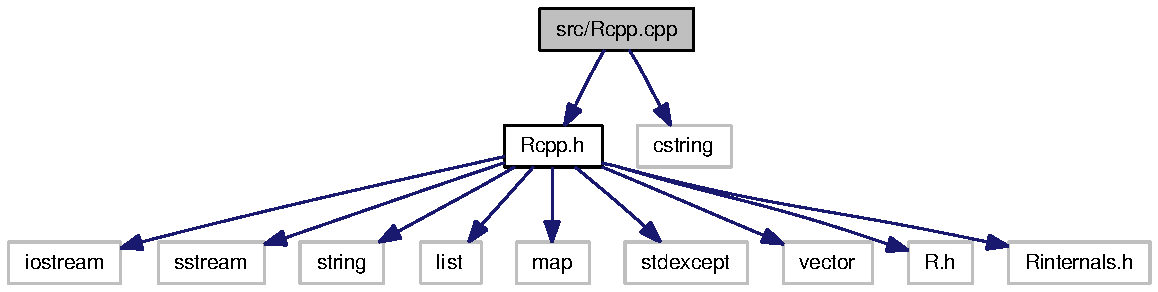
\includegraphics[width=296pt]{Rcpp_8cpp__incl}
\end{center}
\end{figure}
\subsection*{Functions}
\begin{DoxyCompactItemize}
\item 
std::ostream \& \hyperlink{Rcpp_8cpp_a62c075d47528a48e5fb57c1855c4d71c}{operator$<$$<$} (std::ostream \&os, const \hyperlink{classRcppDate}{RcppDate} \&date)
\item 
\hyperlink{classRcppDate}{RcppDate} \hyperlink{Rcpp_8cpp_add881a27c2b8e36897a59bca1d04585f}{operator+} (const \hyperlink{classRcppDate}{RcppDate} \&date, int offset)
\item 
int \hyperlink{Rcpp_8cpp_ae4e7644b1347f6ac24f818357bbe440d}{operator-\/} (const \hyperlink{classRcppDate}{RcppDate} \&date2, const \hyperlink{classRcppDate}{RcppDate} \&date1)
\item 
bool \hyperlink{Rcpp_8cpp_af852d3a1ad52776201f385be5ea18c71}{operator$<$} (const \hyperlink{classRcppDate}{RcppDate} \&date1, const \hyperlink{classRcppDate}{RcppDate} \&date2)
\item 
bool \hyperlink{Rcpp_8cpp_a80164a177c098301c1d509fdab702567}{operator$>$} (const \hyperlink{classRcppDate}{RcppDate} \&date1, const \hyperlink{classRcppDate}{RcppDate} \&date2)
\item 
bool \hyperlink{Rcpp_8cpp_af7a217e1f5d4a91e2d86fc4da858a6c2}{operator$>$=} (const \hyperlink{classRcppDate}{RcppDate} \&date1, const \hyperlink{classRcppDate}{RcppDate} \&date2)
\item 
bool \hyperlink{Rcpp_8cpp_a594132f5ef49b4f477d32289ced4df83}{operator$<$=} (const \hyperlink{classRcppDate}{RcppDate} \&date1, const \hyperlink{classRcppDate}{RcppDate} \&date2)
\item 
bool \hyperlink{Rcpp_8cpp_ad6c1518c6eb9480665f532dbcc6dd2d5}{operator==} (const \hyperlink{classRcppDate}{RcppDate} \&date1, const \hyperlink{classRcppDate}{RcppDate} \&date2)
\item 
char $\ast$ \hyperlink{Rcpp_8cpp_a86330168f60698ba4d745bb97cdbb15b}{copyMessageToR} (const char $\ast$const mesg)
\end{DoxyCompactItemize}


\subsection{Function Documentation}
\hypertarget{Rcpp_8cpp_a86330168f60698ba4d745bb97cdbb15b}{
\index{Rcpp.cpp@{Rcpp.cpp}!copyMessageToR@{copyMessageToR}}
\index{copyMessageToR@{copyMessageToR}!Rcpp.cpp@{Rcpp.cpp}}
\subsubsection[{copyMessageToR}]{\setlength{\rightskip}{0pt plus 5cm}char$\ast$ copyMessageToR (const char $\ast$const  {\em mesg})}}
\label{Rcpp_8cpp_a86330168f60698ba4d745bb97cdbb15b}


Definition at line 1000 of file Rcpp.cpp.

Referenced by Rcpp\_\-Example(), RcppDateExample(), RcppParamsExample(), and RcppVectorExample().\hypertarget{Rcpp_8cpp_add881a27c2b8e36897a59bca1d04585f}{
\index{Rcpp.cpp@{Rcpp.cpp}!operator+@{operator+}}
\index{operator+@{operator+}!Rcpp.cpp@{Rcpp.cpp}}
\subsubsection[{operator+}]{\setlength{\rightskip}{0pt plus 5cm}{\bf RcppDate} operator+ (const {\bf RcppDate} \& {\em date}, \/  int {\em offset})}}
\label{Rcpp_8cpp_add881a27c2b8e36897a59bca1d04585f}


Definition at line 810 of file Rcpp.cpp.

References RcppDate::day, RcppDate::jdn, RcppDate::jdn2mdy(), RcppDate::month, and RcppDate::year.

Here is the call graph for this function:\nopagebreak
\begin{figure}[H]
\begin{center}
\leavevmode
\includegraphics[width=120pt]{Rcpp_8cpp_add881a27c2b8e36897a59bca1d04585f_cgraph}
\end{center}
\end{figure}
\hypertarget{Rcpp_8cpp_ae4e7644b1347f6ac24f818357bbe440d}{
\index{Rcpp.cpp@{Rcpp.cpp}!operator-\/@{operator-\/}}
\index{operator-\/@{operator-\/}!Rcpp.cpp@{Rcpp.cpp}}
\subsubsection[{operator-\/}]{\setlength{\rightskip}{0pt plus 5cm}int operator-\/ (const {\bf RcppDate} \& {\em date2}, \/  const {\bf RcppDate} \& {\em date1})}}
\label{Rcpp_8cpp_ae4e7644b1347f6ac24f818357bbe440d}


Definition at line 817 of file Rcpp.cpp.

References RcppDate::jdn.\hypertarget{Rcpp_8cpp_af852d3a1ad52776201f385be5ea18c71}{
\index{Rcpp.cpp@{Rcpp.cpp}!operator$<$@{operator$<$}}
\index{operator$<$@{operator$<$}!Rcpp.cpp@{Rcpp.cpp}}
\subsubsection[{operator$<$}]{\setlength{\rightskip}{0pt plus 5cm}bool operator$<$ (const {\bf RcppDate} \& {\em date1}, \/  const {\bf RcppDate} \& {\em date2})}}
\label{Rcpp_8cpp_af852d3a1ad52776201f385be5ea18c71}


Definition at line 821 of file Rcpp.cpp.

References RcppDate::jdn.\hypertarget{Rcpp_8cpp_a62c075d47528a48e5fb57c1855c4d71c}{
\index{Rcpp.cpp@{Rcpp.cpp}!operator$<$$<$@{operator$<$$<$}}
\index{operator$<$$<$@{operator$<$$<$}!Rcpp.cpp@{Rcpp.cpp}}
\subsubsection[{operator$<$$<$}]{\setlength{\rightskip}{0pt plus 5cm}std::ostream\& operator$<$$<$ (std::ostream \& {\em os}, \/  const {\bf RcppDate} \& {\em date})}}
\label{Rcpp_8cpp_a62c075d47528a48e5fb57c1855c4d71c}


Definition at line 804 of file Rcpp.cpp.

References RcppDate::getDay(), RcppDate::getMonth(), and RcppDate::getYear().

Here is the call graph for this function:\nopagebreak
\begin{figure}[H]
\begin{center}
\leavevmode
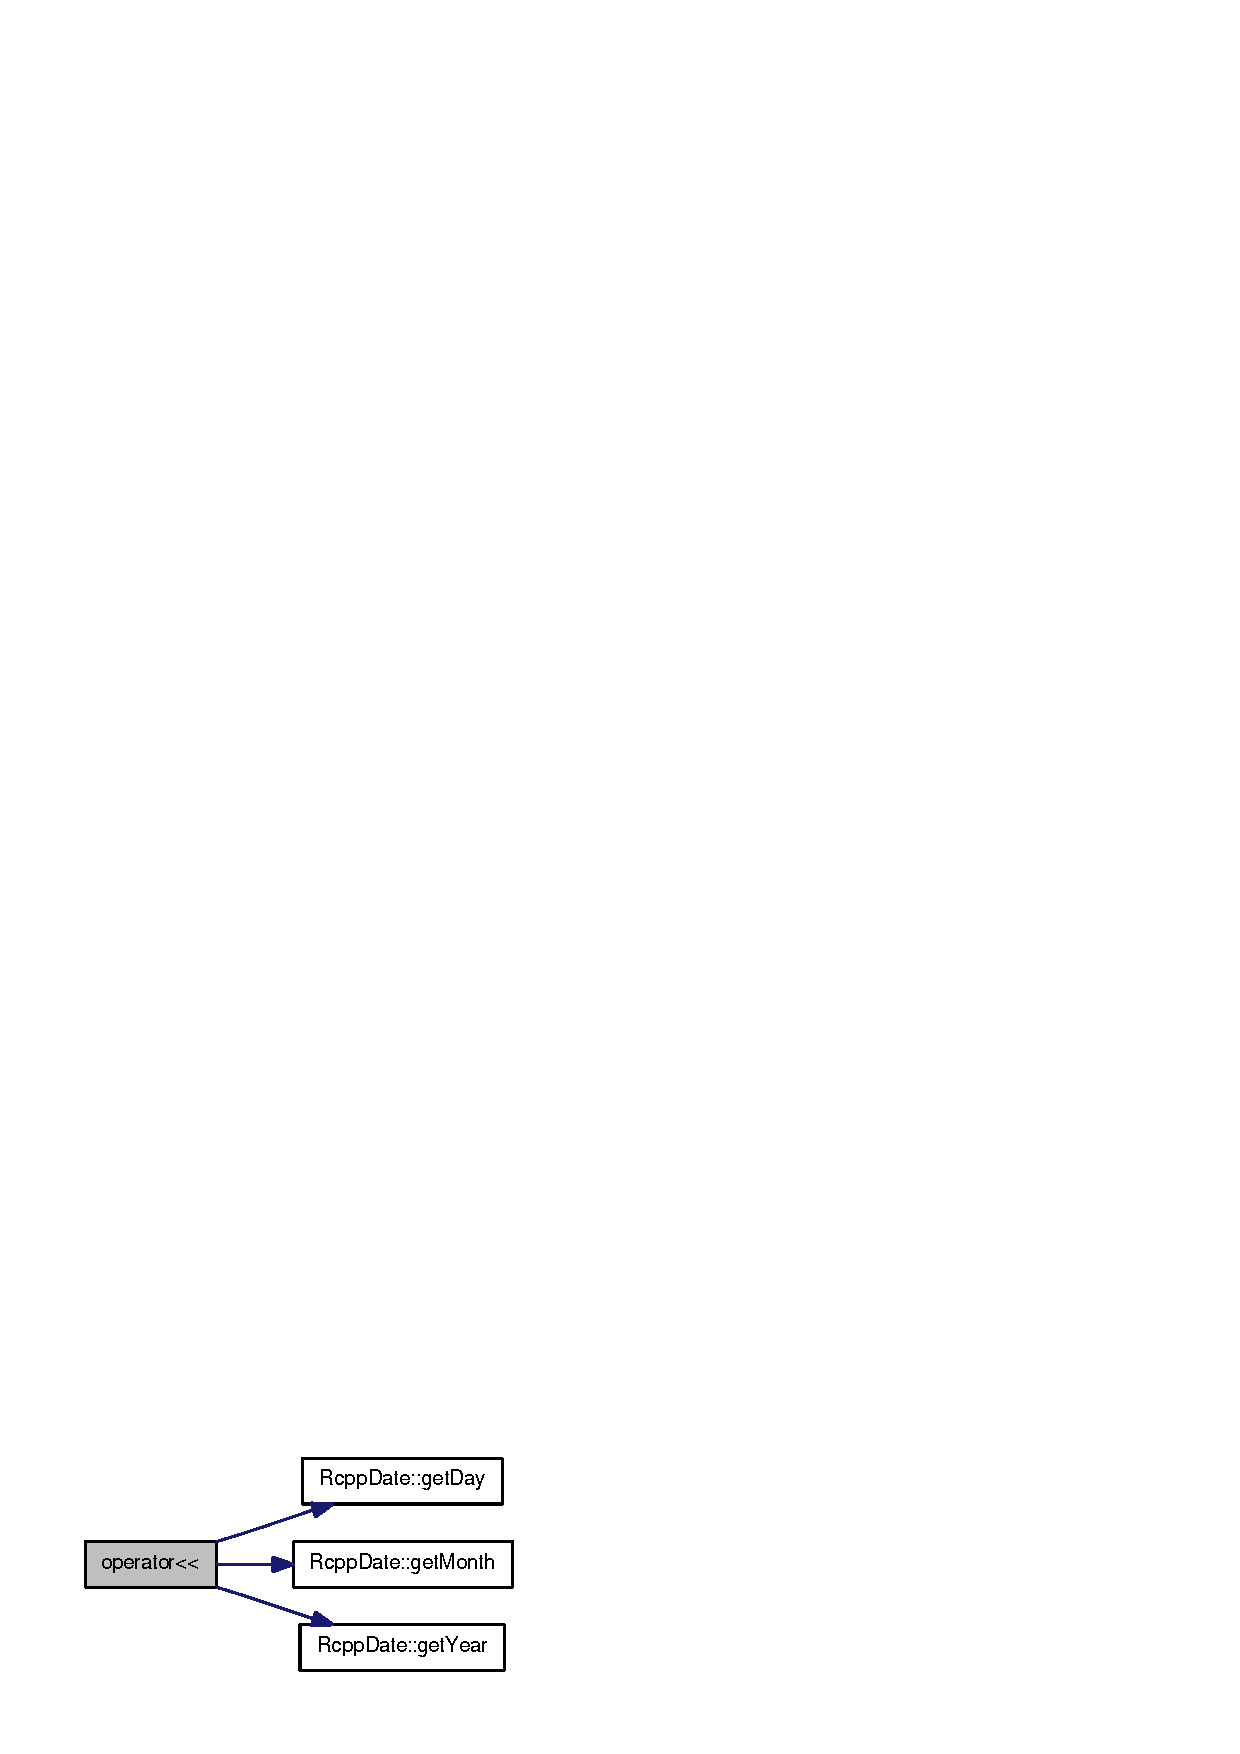
\includegraphics[width=125pt]{Rcpp_8cpp_a62c075d47528a48e5fb57c1855c4d71c_cgraph}
\end{center}
\end{figure}
\hypertarget{Rcpp_8cpp_a594132f5ef49b4f477d32289ced4df83}{
\index{Rcpp.cpp@{Rcpp.cpp}!operator$<$=@{operator$<$=}}
\index{operator$<$=@{operator$<$=}!Rcpp.cpp@{Rcpp.cpp}}
\subsubsection[{operator$<$=}]{\setlength{\rightskip}{0pt plus 5cm}bool operator$<$= (const {\bf RcppDate} \& {\em date1}, \/  const {\bf RcppDate} \& {\em date2})}}
\label{Rcpp_8cpp_a594132f5ef49b4f477d32289ced4df83}


Definition at line 833 of file Rcpp.cpp.

References RcppDate::jdn.\hypertarget{Rcpp_8cpp_ad6c1518c6eb9480665f532dbcc6dd2d5}{
\index{Rcpp.cpp@{Rcpp.cpp}!operator==@{operator==}}
\index{operator==@{operator==}!Rcpp.cpp@{Rcpp.cpp}}
\subsubsection[{operator==}]{\setlength{\rightskip}{0pt plus 5cm}bool operator== (const {\bf RcppDate} \& {\em date1}, \/  const {\bf RcppDate} \& {\em date2})}}
\label{Rcpp_8cpp_ad6c1518c6eb9480665f532dbcc6dd2d5}


Definition at line 837 of file Rcpp.cpp.

References RcppDate::jdn.\hypertarget{Rcpp_8cpp_a80164a177c098301c1d509fdab702567}{
\index{Rcpp.cpp@{Rcpp.cpp}!operator$>$@{operator$>$}}
\index{operator$>$@{operator$>$}!Rcpp.cpp@{Rcpp.cpp}}
\subsubsection[{operator$>$}]{\setlength{\rightskip}{0pt plus 5cm}bool operator$>$ (const {\bf RcppDate} \& {\em date1}, \/  const {\bf RcppDate} \& {\em date2})}}
\label{Rcpp_8cpp_a80164a177c098301c1d509fdab702567}


Definition at line 825 of file Rcpp.cpp.

References RcppDate::jdn.\hypertarget{Rcpp_8cpp_af7a217e1f5d4a91e2d86fc4da858a6c2}{
\index{Rcpp.cpp@{Rcpp.cpp}!operator$>$=@{operator$>$=}}
\index{operator$>$=@{operator$>$=}!Rcpp.cpp@{Rcpp.cpp}}
\subsubsection[{operator$>$=}]{\setlength{\rightskip}{0pt plus 5cm}bool operator$>$= (const {\bf RcppDate} \& {\em date1}, \/  const {\bf RcppDate} \& {\em date2})}}
\label{Rcpp_8cpp_af7a217e1f5d4a91e2d86fc4da858a6c2}


Definition at line 829 of file Rcpp.cpp.

References RcppDate::jdn.
\hypertarget{Rcpp_8h}{
\section{src/Rcpp.h File Reference}
\label{Rcpp_8h}\index{src/Rcpp.h@{src/Rcpp.h}}
}
{\tt \#include $<$iostream$>$}\par
{\tt \#include $<$sstream$>$}\par
{\tt \#include $<$string$>$}\par
{\tt \#include $<$list$>$}\par
{\tt \#include $<$map$>$}\par
{\tt \#include $<$stdexcept$>$}\par
{\tt \#include $<$vector$>$}\par
{\tt \#include $<$R.h$>$}\par
{\tt \#include $<$Rinternals.h$>$}\par


Include dependency graph for Rcpp.h:\nopagebreak
\begin{figure}[H]
\begin{center}
\leavevmode
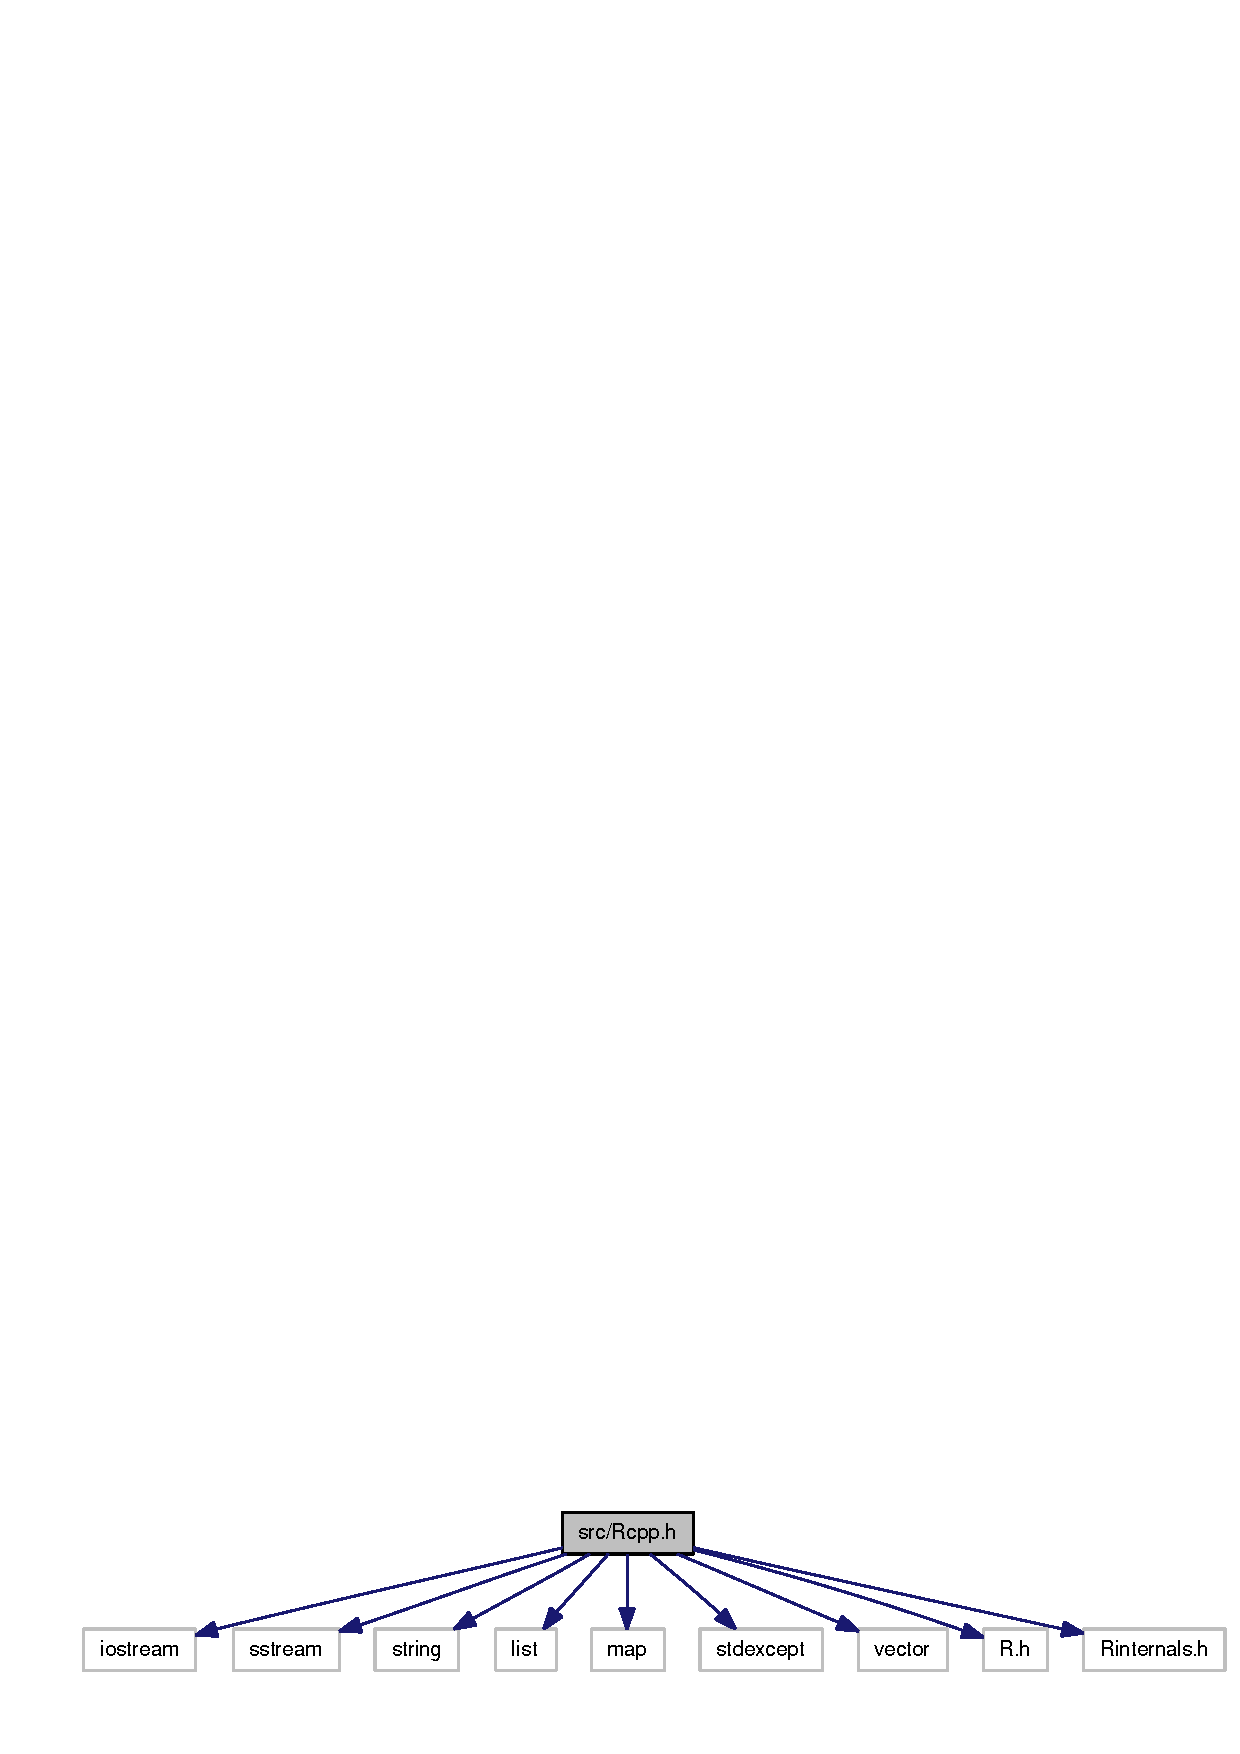
\includegraphics[width=296pt]{Rcpp_8h__incl}
\end{center}
\end{figure}


This graph shows which files directly or indirectly include this file:\nopagebreak
\begin{figure}[H]
\begin{center}
\leavevmode
\includegraphics[width=124pt]{Rcpp_8h__dep__incl}
\end{center}
\end{figure}
\subsection*{Classes}
\begin{CompactItemize}
\item 
class \hyperlink{classRcppDate}{RcppDate}
\item 
class \hyperlink{classRcppDatetime}{RcppDatetime}
\item 
class \hyperlink{classRcppParams}{RcppParams}
\item 
class \hyperlink{classColDatum}{ColDatum}
\item 
class \hyperlink{classRcppFrame}{RcppFrame}
\item 
class \hyperlink{classRcppNumList}{RcppNumList}
\item 
class \hyperlink{classRcppVector}{RcppVector$<$ T $>$}
\item 
class \hyperlink{classRcppStringVector}{RcppStringVector}
\item 
class \hyperlink{classRcppDateVector}{RcppDateVector}
\item 
class \hyperlink{classRcppDatetimeVector}{RcppDatetimeVector}
\item 
class \hyperlink{classRcppMatrix}{RcppMatrix$<$ T $>$}
\item 
class \hyperlink{classRcppVectorView}{RcppVectorView$<$ T $>$}
\item 
class \hyperlink{classRcppMatrixView}{RcppMatrixView$<$ T $>$}
\item 
class \hyperlink{classRcppStringVectorView}{RcppStringVectorView}
\item 
class \hyperlink{classRcppFunction}{RcppFunction}
\item 
class \hyperlink{classRcppResultSet}{RcppResultSet}
\end{CompactItemize}
\subsection*{Defines}
\begin{CompactItemize}
\item 
\#define \hyperlink{Rcpp_8h_367e747a6abc54938d838483bb3c97ee}{R\_\-NO\_\-REMAP}
\item 
\#define \hyperlink{Rcpp_8h_df8c24d3d9680f80efbccf56b0bbcb87}{RcppExport}~extern \char`\"{}C\char`\"{}
\end{CompactItemize}
\subsection*{Enumerations}
\begin{CompactItemize}
\item 
enum \hyperlink{Rcpp_8h_3145f0ed02782c5b592881e0e8e53655}{ColType} \{ \par
\hyperlink{Rcpp_8h_3145f0ed02782c5b592881e0e8e536558033c9699467cc74f87d24c004ca6bff}{COLTYPE\_\-DOUBLE}, 
\hyperlink{Rcpp_8h_3145f0ed02782c5b592881e0e8e536555e594154d950baa0cfa4dca34eec8c4f}{COLTYPE\_\-INT}, 
\hyperlink{Rcpp_8h_3145f0ed02782c5b592881e0e8e5365580fa6b7860dbefb7f6201b10a325a95e}{COLTYPE\_\-STRING}, 
\hyperlink{Rcpp_8h_3145f0ed02782c5b592881e0e8e53655cd671810dc639245baafc3a9ca57a92c}{COLTYPE\_\-FACTOR}, 
\par
\hyperlink{Rcpp_8h_3145f0ed02782c5b592881e0e8e53655bf580a6f2d25cee49648795700ad476d}{COLTYPE\_\-LOGICAL}, 
\hyperlink{Rcpp_8h_3145f0ed02782c5b592881e0e8e53655df2f73e5b0ca56a91699e5e0ba4f945f}{COLTYPE\_\-DATE}, 
\hyperlink{Rcpp_8h_3145f0ed02782c5b592881e0e8e5365505d7e518f4a1811bdb53a7ec4ed3c579}{COLTYPE\_\-DATETIME}
 \}
\end{CompactItemize}
\subsection*{Functions}
\begin{CompactItemize}
\item 
char $\ast$ \hyperlink{Rcpp_8h_86330168f60698ba4d745bb97cdbb15b}{copyMessageToR} (const char $\ast$const mesg)
\end{CompactItemize}


\subsection{Define Documentation}
\hypertarget{Rcpp_8h_367e747a6abc54938d838483bb3c97ee}{
\index{Rcpp.h@{Rcpp.h}!R\_\-NO\_\-REMAP@{R\_\-NO\_\-REMAP}}
\index{R\_\-NO\_\-REMAP@{R\_\-NO\_\-REMAP}!Rcpp.h@{Rcpp.h}}
\subsubsection[{R\_\-NO\_\-REMAP}]{\setlength{\rightskip}{0pt plus 5cm}\#define R\_\-NO\_\-REMAP}}
\label{Rcpp_8h_367e747a6abc54938d838483bb3c97ee}




Definition at line 34 of file Rcpp.h.\hypertarget{Rcpp_8h_df8c24d3d9680f80efbccf56b0bbcb87}{
\index{Rcpp.h@{Rcpp.h}!RcppExport@{RcppExport}}
\index{RcppExport@{RcppExport}!Rcpp.h@{Rcpp.h}}
\subsubsection[{RcppExport}]{\setlength{\rightskip}{0pt plus 5cm}\#define RcppExport~extern \char`\"{}C\char`\"{}}}
\label{Rcpp_8h_df8c24d3d9680f80efbccf56b0bbcb87}




Definition at line 42 of file Rcpp.h.

\subsection{Enumeration Type Documentation}
\hypertarget{Rcpp_8h_3145f0ed02782c5b592881e0e8e53655}{
\index{Rcpp.h@{Rcpp.h}!ColType@{ColType}}
\index{ColType@{ColType}!Rcpp.h@{Rcpp.h}}
\subsubsection[{ColType}]{\setlength{\rightskip}{0pt plus 5cm}enum {\bf ColType}}}
\label{Rcpp_8h_3145f0ed02782c5b592881e0e8e53655}


\begin{Desc}
\item[Enumerator: ]\par
\begin{description}
\index{COLTYPE\_\-DOUBLE@{COLTYPE\_\-DOUBLE}!Rcpp.h@{Rcpp.h}}\index{Rcpp.h@{Rcpp.h}!COLTYPE\_\-DOUBLE@{COLTYPE\_\-DOUBLE}}\item[{\em 
\hypertarget{Rcpp_8h_3145f0ed02782c5b592881e0e8e536558033c9699467cc74f87d24c004ca6bff}{
COLTYPE\_\-DOUBLE}
\label{Rcpp_8h_3145f0ed02782c5b592881e0e8e536558033c9699467cc74f87d24c004ca6bff}
}]\index{COLTYPE\_\-INT@{COLTYPE\_\-INT}!Rcpp.h@{Rcpp.h}}\index{Rcpp.h@{Rcpp.h}!COLTYPE\_\-INT@{COLTYPE\_\-INT}}\item[{\em 
\hypertarget{Rcpp_8h_3145f0ed02782c5b592881e0e8e536555e594154d950baa0cfa4dca34eec8c4f}{
COLTYPE\_\-INT}
\label{Rcpp_8h_3145f0ed02782c5b592881e0e8e536555e594154d950baa0cfa4dca34eec8c4f}
}]\index{COLTYPE\_\-STRING@{COLTYPE\_\-STRING}!Rcpp.h@{Rcpp.h}}\index{Rcpp.h@{Rcpp.h}!COLTYPE\_\-STRING@{COLTYPE\_\-STRING}}\item[{\em 
\hypertarget{Rcpp_8h_3145f0ed02782c5b592881e0e8e5365580fa6b7860dbefb7f6201b10a325a95e}{
COLTYPE\_\-STRING}
\label{Rcpp_8h_3145f0ed02782c5b592881e0e8e5365580fa6b7860dbefb7f6201b10a325a95e}
}]\index{COLTYPE\_\-FACTOR@{COLTYPE\_\-FACTOR}!Rcpp.h@{Rcpp.h}}\index{Rcpp.h@{Rcpp.h}!COLTYPE\_\-FACTOR@{COLTYPE\_\-FACTOR}}\item[{\em 
\hypertarget{Rcpp_8h_3145f0ed02782c5b592881e0e8e53655cd671810dc639245baafc3a9ca57a92c}{
COLTYPE\_\-FACTOR}
\label{Rcpp_8h_3145f0ed02782c5b592881e0e8e53655cd671810dc639245baafc3a9ca57a92c}
}]\index{COLTYPE\_\-LOGICAL@{COLTYPE\_\-LOGICAL}!Rcpp.h@{Rcpp.h}}\index{Rcpp.h@{Rcpp.h}!COLTYPE\_\-LOGICAL@{COLTYPE\_\-LOGICAL}}\item[{\em 
\hypertarget{Rcpp_8h_3145f0ed02782c5b592881e0e8e53655bf580a6f2d25cee49648795700ad476d}{
COLTYPE\_\-LOGICAL}
\label{Rcpp_8h_3145f0ed02782c5b592881e0e8e53655bf580a6f2d25cee49648795700ad476d}
}]\index{COLTYPE\_\-DATE@{COLTYPE\_\-DATE}!Rcpp.h@{Rcpp.h}}\index{Rcpp.h@{Rcpp.h}!COLTYPE\_\-DATE@{COLTYPE\_\-DATE}}\item[{\em 
\hypertarget{Rcpp_8h_3145f0ed02782c5b592881e0e8e53655df2f73e5b0ca56a91699e5e0ba4f945f}{
COLTYPE\_\-DATE}
\label{Rcpp_8h_3145f0ed02782c5b592881e0e8e53655df2f73e5b0ca56a91699e5e0ba4f945f}
}]\index{COLTYPE\_\-DATETIME@{COLTYPE\_\-DATETIME}!Rcpp.h@{Rcpp.h}}\index{Rcpp.h@{Rcpp.h}!COLTYPE\_\-DATETIME@{COLTYPE\_\-DATETIME}}\item[{\em 
\hypertarget{Rcpp_8h_3145f0ed02782c5b592881e0e8e5365505d7e518f4a1811bdb53a7ec4ed3c579}{
COLTYPE\_\-DATETIME}
\label{Rcpp_8h_3145f0ed02782c5b592881e0e8e5365505d7e518f4a1811bdb53a7ec4ed3c579}
}]\end{description}
\end{Desc}



Definition at line 167 of file Rcpp.h.

\subsection{Function Documentation}
\hypertarget{Rcpp_8h_86330168f60698ba4d745bb97cdbb15b}{
\index{Rcpp.h@{Rcpp.h}!copyMessageToR@{copyMessageToR}}
\index{copyMessageToR@{copyMessageToR}!Rcpp.h@{Rcpp.h}}
\subsubsection[{copyMessageToR}]{\setlength{\rightskip}{0pt plus 5cm}char$\ast$ copyMessageToR (const char $\ast$const  {\em mesg})}}
\label{Rcpp_8h_86330168f60698ba4d745bb97cdbb15b}




Definition at line 995 of file Rcpp.cpp.

Referenced by Rcpp\_\-Example(), RcppDateExample(), RcppParamsExample(), and RcppVectorExample().
\hypertarget{RcppExample_8cpp}{
\section{src/RcppExample.cpp File Reference}
\label{RcppExample_8cpp}\index{src/RcppExample.cpp@{src/RcppExample.cpp}}
}
{\tt \#include \char`\"{}Rcpp.h\char`\"{}}\par


Include dependency graph for RcppExample.cpp:\nopagebreak
\begin{figure}[H]
\begin{center}
\leavevmode
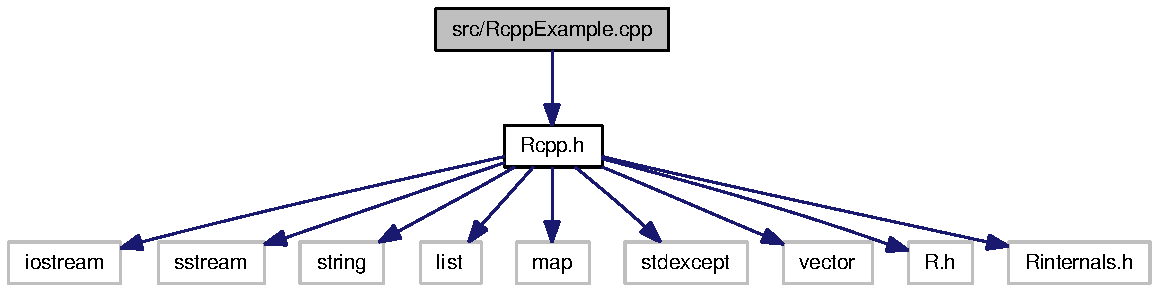
\includegraphics[width=296pt]{RcppExample_8cpp__incl}
\end{center}
\end{figure}
\subsection*{Classes}
\begin{CompactItemize}
\item 
class \hyperlink{classMyRVectorFunc}{MyRVectorFunc}
\item 
class \hyperlink{classMyRListFunc}{MyRListFunc}
\end{CompactItemize}
\subsection*{Functions}
\begin{CompactItemize}
\item 
RcppExport SEXP \hyperlink{RcppExample_8cpp_f892bc38cc3c6c75840941c5d27a316f}{Rcpp\_\-Example} (SEXP params, SEXP nlist, SEXP numvec, SEXP nummat, SEXP df, SEXP datevec, SEXP stringvec, SEXP fnvec, SEXP fnlist)
\item 
RcppExport SEXP \hyperlink{RcppExample_8cpp_44dbfa080dcf3c7ed95e7d0b067276b3}{RcppParamsExample} (SEXP params)
\item 
RcppExport SEXP \hyperlink{RcppExample_8cpp_ecc07b10373d7134c6be02aaa652fc19}{RcppDateExample} (SEXP dvsexp, SEXP dtvsexp)
\item 
RcppExport SEXP \hyperlink{RcppExample_8cpp_4d13d94df70a9a51d67cc6546eb2454f}{RcppVectorExample} (SEXP vector)
\end{CompactItemize}


\subsection{Function Documentation}
\hypertarget{RcppExample_8cpp_f892bc38cc3c6c75840941c5d27a316f}{
\index{RcppExample.cpp@{RcppExample.cpp}!Rcpp\_\-Example@{Rcpp\_\-Example}}
\index{Rcpp\_\-Example@{Rcpp\_\-Example}!RcppExample.cpp@{RcppExample.cpp}}
\subsubsection[{Rcpp\_\-Example}]{\setlength{\rightskip}{0pt plus 5cm}RcppExport SEXP Rcpp\_\-Example (SEXP {\em params}, \/  SEXP {\em nlist}, \/  SEXP {\em numvec}, \/  SEXP {\em nummat}, \/  SEXP {\em df}, \/  SEXP {\em datevec}, \/  SEXP {\em stringvec}, \/  SEXP {\em fnvec}, \/  SEXP {\em fnlist})}}
\label{RcppExample_8cpp_f892bc38cc3c6c75840941c5d27a316f}




Definition at line 109 of file RcppExample.cpp.

References RcppResultSet::add(), MyRListFunc::addOne(), RcppFrame::addRow(), RcppMatrix$<$ T $>$::cMatrix(), copyMessageToR(), RcppVector$<$ T $>$::cVector(), RcppParams::getDateValue(), RcppDate::getDay(), RcppMatrix$<$ T $>$::getDim1(), RcppMatrix$<$ T $>$::getDim2(), RcppParams::getDoubleValue(), RcppParams::getIntValue(), RcppDate::getMonth(), RcppNumList::getName(), RcppResultSet::getReturnList(), RcppParams::getStringValue(), MyRVectorFunc::getSum(), RcppNumList::getValue(), RcppDate::getYear(), RcppVector$<$ T $>$::size(), RcppMatrix$<$ T $>$::stlMatrix(), and RcppVector$<$ T $>$::stlVector().

Here is the call graph for this function:\nopagebreak
\begin{figure}[H]
\begin{center}
\leavevmode
\includegraphics[width=259pt]{RcppExample_8cpp_f892bc38cc3c6c75840941c5d27a316f_cgraph}
\end{center}
\end{figure}
\hypertarget{RcppExample_8cpp_ecc07b10373d7134c6be02aaa652fc19}{
\index{RcppExample.cpp@{RcppExample.cpp}!RcppDateExample@{RcppDateExample}}
\index{RcppDateExample@{RcppDateExample}!RcppExample.cpp@{RcppExample.cpp}}
\subsubsection[{RcppDateExample}]{\setlength{\rightskip}{0pt plus 5cm}RcppExport SEXP RcppDateExample (SEXP {\em dvsexp}, \/  SEXP {\em dtvsexp})}}
\label{RcppExample_8cpp_ecc07b10373d7134c6be02aaa652fc19}




Definition at line 382 of file RcppExample.cpp.

References RcppResultSet::add(), copyMessageToR(), RcppResultSet::getReturnList(), RcppDatetimeVector::size(), and RcppDateVector::size().

Here is the call graph for this function:\nopagebreak
\begin{figure}[H]
\begin{center}
\leavevmode
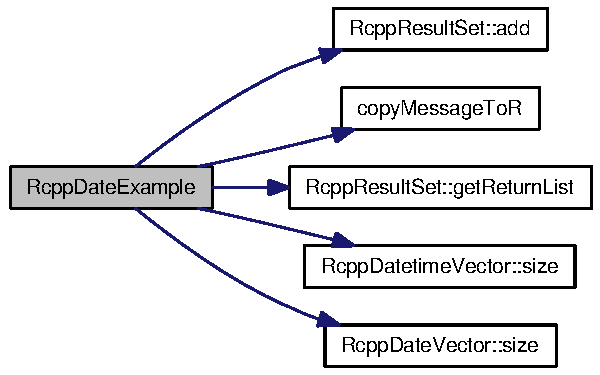
\includegraphics[width=162pt]{RcppExample_8cpp_ecc07b10373d7134c6be02aaa652fc19_cgraph}
\end{center}
\end{figure}
\hypertarget{RcppExample_8cpp_44dbfa080dcf3c7ed95e7d0b067276b3}{
\index{RcppExample.cpp@{RcppExample.cpp}!RcppParamsExample@{RcppParamsExample}}
\index{RcppParamsExample@{RcppParamsExample}!RcppExample.cpp@{RcppExample.cpp}}
\subsubsection[{RcppParamsExample}]{\setlength{\rightskip}{0pt plus 5cm}RcppExport SEXP RcppParamsExample (SEXP {\em params})}}
\label{RcppExample_8cpp_44dbfa080dcf3c7ed95e7d0b067276b3}




Definition at line 333 of file RcppExample.cpp.

References copyMessageToR(), RcppParams::getDateValue(), RcppDate::getDay(), RcppParams::getDoubleValue(), RcppParams::getIntValue(), RcppDate::getMonth(), RcppParams::getStringValue(), and RcppDate::getYear().

Here is the call graph for this function:\nopagebreak
\begin{figure}[H]
\begin{center}
\leavevmode
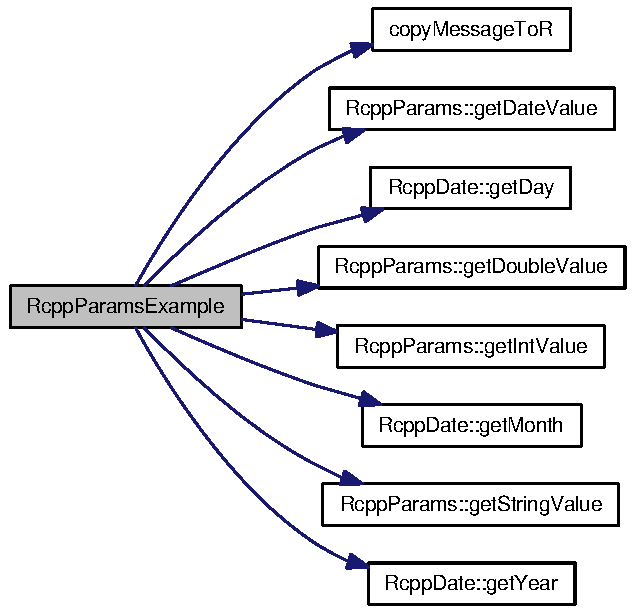
\includegraphics[width=169pt]{RcppExample_8cpp_44dbfa080dcf3c7ed95e7d0b067276b3_cgraph}
\end{center}
\end{figure}
\hypertarget{RcppExample_8cpp_4d13d94df70a9a51d67cc6546eb2454f}{
\index{RcppExample.cpp@{RcppExample.cpp}!RcppVectorExample@{RcppVectorExample}}
\index{RcppVectorExample@{RcppVectorExample}!RcppExample.cpp@{RcppExample.cpp}}
\subsubsection[{RcppVectorExample}]{\setlength{\rightskip}{0pt plus 5cm}RcppExport SEXP RcppVectorExample (SEXP {\em vector})}}
\label{RcppExample_8cpp_4d13d94df70a9a51d67cc6546eb2454f}




Definition at line 423 of file RcppExample.cpp.

References RcppResultSet::add(), copyMessageToR(), RcppResultSet::getReturnList(), and RcppVector$<$ T $>$::size().

Here is the call graph for this function:\nopagebreak
\begin{figure}[H]
\begin{center}
\leavevmode
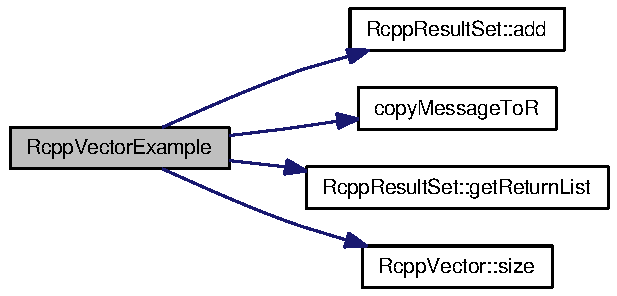
\includegraphics[width=166pt]{RcppExample_8cpp_4d13d94df70a9a51d67cc6546eb2454f_cgraph}
\end{center}
\end{figure}

\printindex
\end{document}
